\documentclass[twoside]{book}

% Packages required by doxygen
\usepackage{fixltx2e}
\usepackage{calc}
\usepackage{doxygen}
\usepackage[export]{adjustbox} % also loads graphicx
\usepackage{graphicx}
\usepackage[utf8]{inputenc}
\usepackage{makeidx}
\usepackage{multicol}
\usepackage{multirow}
\PassOptionsToPackage{warn}{textcomp}
\usepackage{textcomp}
\usepackage[nointegrals]{wasysym}
\usepackage[table]{xcolor}

% Font selection
\usepackage[T1]{fontenc}
\usepackage[scaled=.90]{helvet}
\usepackage{courier}
\usepackage{amssymb}
\usepackage{sectsty}
\renewcommand{\familydefault}{\sfdefault}
\allsectionsfont{%
  \fontseries{bc}\selectfont%
  \color{darkgray}%
}
\renewcommand{\DoxyLabelFont}{%
  \fontseries{bc}\selectfont%
  \color{darkgray}%
}
\newcommand{\+}{\discretionary{\mbox{\scriptsize$\hookleftarrow$}}{}{}}

% Page & text layout
\usepackage{geometry}
\geometry{%
  a4paper,%
  top=2.5cm,%
  bottom=2.5cm,%
  left=2.5cm,%
  right=2.5cm%
}
\tolerance=750
\hfuzz=15pt
\hbadness=750
\setlength{\emergencystretch}{15pt}
\setlength{\parindent}{0cm}
\setlength{\parskip}{3ex plus 2ex minus 2ex}
\makeatletter
\renewcommand{\paragraph}{%
  \@startsection{paragraph}{4}{0ex}{-1.0ex}{1.0ex}{%
    \normalfont\normalsize\bfseries\SS@parafont%
  }%
}
\renewcommand{\subparagraph}{%
  \@startsection{subparagraph}{5}{0ex}{-1.0ex}{1.0ex}{%
    \normalfont\normalsize\bfseries\SS@subparafont%
  }%
}
\makeatother

% Headers & footers
\usepackage{fancyhdr}
\pagestyle{fancyplain}
\fancyhead[LE]{\fancyplain{}{\bfseries\thepage}}
\fancyhead[CE]{\fancyplain{}{}}
\fancyhead[RE]{\fancyplain{}{\bfseries\leftmark}}
\fancyhead[LO]{\fancyplain{}{\bfseries\rightmark}}
\fancyhead[CO]{\fancyplain{}{}}
\fancyhead[RO]{\fancyplain{}{\bfseries\thepage}}
\fancyfoot[LE]{\fancyplain{}{}}
\fancyfoot[CE]{\fancyplain{}{}}
\fancyfoot[RE]{\fancyplain{}{\bfseries\scriptsize Generated by Doxygen }}
\fancyfoot[LO]{\fancyplain{}{\bfseries\scriptsize Generated by Doxygen }}
\fancyfoot[CO]{\fancyplain{}{}}
\fancyfoot[RO]{\fancyplain{}{}}
\renewcommand{\footrulewidth}{0.4pt}
\renewcommand{\chaptermark}[1]{%
  \markboth{#1}{}%
}
\renewcommand{\sectionmark}[1]{%
  \markright{\thesection\ #1}%
}

% Indices & bibliography
\usepackage{natbib}
\usepackage[titles]{tocloft}
\setcounter{tocdepth}{3}
\setcounter{secnumdepth}{5}
\makeindex

% Hyperlinks (required, but should be loaded last)
\usepackage{ifpdf}
\ifpdf
  \usepackage[pdftex,pagebackref=true]{hyperref}
\else
  \usepackage[ps2pdf,pagebackref=true]{hyperref}
\fi
\hypersetup{%
  colorlinks=true,%
  linkcolor=blue,%
  citecolor=blue,%
  unicode%
}

% Custom commands
\newcommand{\clearemptydoublepage}{%
  \newpage{\pagestyle{empty}\cleardoublepage}%
}

\usepackage{caption}
\captionsetup{labelsep=space,justification=centering,font={bf},singlelinecheck=off,skip=4pt,position=top}

%===== C O N T E N T S =====

\begin{document}

% Titlepage & ToC
\hypersetup{pageanchor=false,
             bookmarksnumbered=true,
             pdfencoding=unicode
            }
\pagenumbering{alph}
\begin{titlepage}
\vspace*{7cm}
\begin{center}%
{\Large I\+GM -\/ Re\+Con\+Bot \\[1ex]\large 2 }\\
\vspace*{1cm}
{\large Generated by Doxygen 1.8.13}\\
\end{center}
\end{titlepage}
\clearemptydoublepage
\pagenumbering{roman}
\tableofcontents
\clearemptydoublepage
\pagenumbering{arabic}
\hypersetup{pageanchor=true}

%--- Begin generated contents ---
\chapter{Main Page}
\label{index}\hypertarget{index}{}This is a Package which has been created aimed in the control of the I\+GM\textquotesingle{}s U\+R5. Here you will find several scripts which are part of the I\+GM (R\+W\+TH Aachen University) repository for different robots which works together as a part of a R\+OS network.

\begin{DoxyAuthor}{Author}
Jorge De La Cruz 
\end{DoxyAuthor}
\begin{DoxyVersion}{Version}
1.\+0 
\end{DoxyVersion}
\begin{DoxyDate}{Date}
February 28, 2017 
\end{DoxyDate}

\chapter{This is the title of the markdown}
\label{md__home_jdelacruz_catkin_ws_src_reconbot_reconbot_control_docs_main}
\Hypertarget{md__home_jdelacruz_catkin_ws_src_reconbot_reconbot_control_docs_main}
This is a file about teh \hyperlink{class_re_con_bot}{Re\+Con\+Bot} 
\chapter{Namespace Index}
\section{Namespace List}
Here is a list of all namespaces with brief descriptions\+:\begin{DoxyCompactList}
\item\contentsline{section}{\hyperlink{namespacesetup}{setup} }{\pageref{namespacesetup}}{}
\item\contentsline{section}{\hyperlink{namespacetrajectory__client}{trajectory\+\_\+client} }{\pageref{namespacetrajectory__client}}{}
\end{DoxyCompactList}

\chapter{Hierarchical Index}
\section{Class Hierarchy}
This inheritance list is sorted roughly, but not completely, alphabetically\+:\begin{DoxyCompactList}
\item \contentsline{section}{trajectory\+\_\+client.\+Joint}{\pageref{classtrajectory__client_1_1_joint}}{}
\item \contentsline{section}{Re\+Con\+Bot}{\pageref{class_re_con_bot}}{}
\begin{DoxyCompactList}
\item \contentsline{section}{Re\+Con\+Bot\+Lx}{\pageref{class_re_con_bot_lx}}{}
\begin{DoxyCompactList}
\item \contentsline{section}{Re\+Con\+Bot\+Pub}{\pageref{class_re_con_bot_pub}}{}
\end{DoxyCompactList}
\end{DoxyCompactList}
\item \contentsline{section}{Re\+Con\+Bot\+Arm}{\pageref{class_re_con_bot_arm}}{}
\end{DoxyCompactList}

\chapter{Class Index}
\section{Class List}
Here are the classes, structs, unions and interfaces with brief descriptions\+:\begin{DoxyCompactList}
\item\contentsline{section}{\hyperlink{classtrajectory__client_1_1_joint}{trajectory\+\_\+client.\+Joint} }{\pageref{classtrajectory__client_1_1_joint}}{}
\item\contentsline{section}{\hyperlink{class_re_con_bot}{Re\+Con\+Bot} \\*Class implemented for driving the \hyperlink{class_re_con_bot}{Re\+Con\+Bot} planning group }{\pageref{class_re_con_bot}}{}
\item\contentsline{section}{\hyperlink{class_re_con_bot_arm}{Re\+Con\+Bot\+Arm} }{\pageref{class_re_con_bot_arm}}{}
\item\contentsline{section}{\hyperlink{class_re_con_bot_lx}{Re\+Con\+Bot\+Lx} }{\pageref{class_re_con_bot_lx}}{}
\item\contentsline{section}{\hyperlink{class_re_con_bot_pub}{Re\+Con\+Bot\+Pub} }{\pageref{class_re_con_bot_pub}}{}
\end{DoxyCompactList}

\chapter{File Index}
\section{File List}
Here is a list of all files with brief descriptions\+:\begin{DoxyCompactList}
\item\contentsline{section}{\hyperlink{basic__arm_8cpp}{basic\+\_\+arm.\+cpp} }{\pageref{basic__arm_8cpp}}{}
\item\contentsline{section}{\hyperlink{l__arm__move__group__interface_8cpp}{l\+\_\+arm\+\_\+move\+\_\+group\+\_\+interface.\+cpp} }{\pageref{l__arm__move__group__interface_8cpp}}{}
\item\contentsline{section}{\hyperlink{l__arm__trajectory__publisher_8cpp}{l\+\_\+arm\+\_\+trajectory\+\_\+publisher.\+cpp} }{\pageref{l__arm__trajectory__publisher_8cpp}}{}
\item\contentsline{section}{\hyperlink{move__group__interface_8cpp}{move\+\_\+group\+\_\+interface.\+cpp} }{\pageref{move__group__interface_8cpp}}{}
\item\contentsline{section}{\hyperlink{r__arm__move__group__interface_8cpp}{r\+\_\+arm\+\_\+move\+\_\+group\+\_\+interface.\+cpp} }{\pageref{r__arm__move__group__interface_8cpp}}{}
\item\contentsline{section}{\hyperlink{r__arm__trajectory__publisher_8cpp}{r\+\_\+arm\+\_\+trajectory\+\_\+publisher.\+cpp} }{\pageref{r__arm__trajectory__publisher_8cpp}}{}
\item\contentsline{section}{\hyperlink{_re_con_bot_8h}{Re\+Con\+Bot.\+h} }{\pageref{_re_con_bot_8h}}{}
\item\contentsline{section}{\hyperlink{setup_8py}{setup.\+py} }{\pageref{setup_8py}}{}
\item\contentsline{section}{\hyperlink{trajectory__client_8py}{trajectory\+\_\+client.\+py} }{\pageref{trajectory__client_8py}}{}
\item\contentsline{section}{\hyperlink{trajectory__publisher_8cpp}{trajectory\+\_\+publisher.\+cpp} }{\pageref{trajectory__publisher_8cpp}}{}
\end{DoxyCompactList}

\chapter{Namespace Documentation}
\hypertarget{namespacesetup}{}\section{setup Namespace Reference}
\label{namespacesetup}\index{setup@{setup}}
\subsection*{Variables}
\begin{DoxyCompactItemize}
\item 
\hyperlink{namespacesetup_aa2586b6c4dd84a0aaaf49cb1565cee6e}{d}
\end{DoxyCompactItemize}


\subsection{Variable Documentation}
\mbox{\Hypertarget{namespacesetup_aa2586b6c4dd84a0aaaf49cb1565cee6e}\label{namespacesetup_aa2586b6c4dd84a0aaaf49cb1565cee6e}} 
\index{setup@{setup}!d@{d}}
\index{d@{d}!setup@{setup}}
\subsubsection{\texorpdfstring{d}{d}}
{\footnotesize\ttfamily setup.\+d}

{\bfseries Initial value\+:}
\begin{DoxyCode}
1 =  generate\_distutils\_setup(
2     packages=[\textcolor{stringliteral}{'reconbot\_control'}],
3     package\_dir=\{\textcolor{stringliteral}{''}: \textcolor{stringliteral}{'src'}\},
4     )
\end{DoxyCode}


Definition at line 6 of file setup.\+py.


\hypertarget{namespacetrajectory__client}{}\section{trajectory\+\_\+client Namespace Reference}
\label{namespacetrajectory__client}\index{trajectory\+\_\+client@{trajectory\+\_\+client}}
\subsection*{Classes}
\begin{DoxyCompactItemize}
\item 
class \hyperlink{classtrajectory__client_1_1_joint}{Joint}
\end{DoxyCompactItemize}
\subsection*{Functions}
\begin{DoxyCompactItemize}
\item 
def \hyperlink{namespacetrajectory__client_a02f1f1cd99c608b8ea5167cb3c52a485}{main} ()
\end{DoxyCompactItemize}


\subsection{Function Documentation}
\mbox{\Hypertarget{namespacetrajectory__client_a02f1f1cd99c608b8ea5167cb3c52a485}\label{namespacetrajectory__client_a02f1f1cd99c608b8ea5167cb3c52a485}} 
\index{trajectory\+\_\+client@{trajectory\+\_\+client}!main@{main}}
\index{main@{main}!trajectory\+\_\+client@{trajectory\+\_\+client}}
\subsubsection{\texorpdfstring{main()}{main()}}
{\footnotesize\ttfamily def trajectory\+\_\+client.\+main (\begin{DoxyParamCaption}{ }\end{DoxyParamCaption})}



Definition at line 36 of file trajectory\+\_\+client.\+py.


\begin{DoxyCode}
36 \textcolor{keyword}{def }\hyperlink{namespacetrajectory__client_a02f1f1cd99c608b8ea5167cb3c52a485}{main}():
37             arm = Joint(\textcolor{stringliteral}{'arm\_reconbot'})
38             arm.move\_joint([0.0,0.0,0.0])
39             \textcolor{comment}{#arm.move\_joint([0.5,0.5,0.5])}
40             \textcolor{comment}{#arm.move\_joint([1.0,1.0,1.0])}
41             \textcolor{comment}{#arm.move\_joint([1.5,1.5,1.5])}
42             \textcolor{comment}{#arm.move\_joint([2.0,2.0,2.0])}
43 
44 
\end{DoxyCode}

\chapter{Class Documentation}
\hypertarget{classtrajectory__client_1_1_joint}{}\section{trajectory\+\_\+client.\+Joint Class Reference}
\label{classtrajectory__client_1_1_joint}\index{trajectory\+\_\+client.\+Joint@{trajectory\+\_\+client.\+Joint}}
\subsection*{Public Member Functions}
\begin{DoxyCompactItemize}
\item 
def \hyperlink{classtrajectory__client_1_1_joint_a9d389b66ef367799eb9141b9b107dc9f}{\+\_\+\+\_\+init\+\_\+\+\_\+} (self, motor\+\_\+name)
\item 
def \hyperlink{classtrajectory__client_1_1_joint_a0d8109140ca6092a4fa5e92fe75aaeb9}{move\+\_\+joint} (self, angles)
\end{DoxyCompactItemize}
\subsection*{Public Attributes}
\begin{DoxyCompactItemize}
\item 
\hyperlink{classtrajectory__client_1_1_joint_a1b9ed73437add9c5b106edf224295b7e}{name}
\item 
\hyperlink{classtrajectory__client_1_1_joint_a749e573716c2744874918f2e7b00c33a}{jta}
\end{DoxyCompactItemize}


\subsection{Detailed Description}


Definition at line 15 of file trajectory\+\_\+client.\+py.



\subsection{Constructor \& Destructor Documentation}
\mbox{\Hypertarget{classtrajectory__client_1_1_joint_a9d389b66ef367799eb9141b9b107dc9f}\label{classtrajectory__client_1_1_joint_a9d389b66ef367799eb9141b9b107dc9f}} 
\index{trajectory\+\_\+client\+::\+Joint@{trajectory\+\_\+client\+::\+Joint}!\+\_\+\+\_\+init\+\_\+\+\_\+@{\+\_\+\+\_\+init\+\_\+\+\_\+}}
\index{\+\_\+\+\_\+init\+\_\+\+\_\+@{\+\_\+\+\_\+init\+\_\+\+\_\+}!trajectory\+\_\+client\+::\+Joint@{trajectory\+\_\+client\+::\+Joint}}
\subsubsection{\texorpdfstring{\+\_\+\+\_\+init\+\_\+\+\_\+()}{\_\_init\_\_()}}
{\footnotesize\ttfamily def trajectory\+\_\+client.\+Joint.\+\_\+\+\_\+init\+\_\+\+\_\+ (\begin{DoxyParamCaption}\item[{}]{self,  }\item[{}]{motor\+\_\+name }\end{DoxyParamCaption})}



Definition at line 16 of file trajectory\+\_\+client.\+py.


\begin{DoxyCode}
16         \textcolor{keyword}{def }\_\_init\_\_(self, motor\_name):
17             \textcolor{comment}{#arm\_name should be b\_arm or f\_arm}
18             self.name = motor\_name
19             self.jta = actionlib.SimpleActionClient(\textcolor{stringliteral}{'/'}+self.name+\textcolor{stringliteral}{'\_controller/follow\_joint\_trajectory'}, 
      FollowJointTrajectoryAction)
20             rospy.loginfo(\textcolor{stringliteral}{'Waiting for joint trajectory action'})
21             self.jta.wait\_for\_server()
22             rospy.loginfo(\textcolor{stringliteral}{'Found joint trajectory action!'})
23 
24 
\end{DoxyCode}


\subsection{Member Function Documentation}
\mbox{\Hypertarget{classtrajectory__client_1_1_joint_a0d8109140ca6092a4fa5e92fe75aaeb9}\label{classtrajectory__client_1_1_joint_a0d8109140ca6092a4fa5e92fe75aaeb9}} 
\index{trajectory\+\_\+client\+::\+Joint@{trajectory\+\_\+client\+::\+Joint}!move\+\_\+joint@{move\+\_\+joint}}
\index{move\+\_\+joint@{move\+\_\+joint}!trajectory\+\_\+client\+::\+Joint@{trajectory\+\_\+client\+::\+Joint}}
\subsubsection{\texorpdfstring{move\+\_\+joint()}{move\_joint()}}
{\footnotesize\ttfamily def trajectory\+\_\+client.\+Joint.\+move\+\_\+joint (\begin{DoxyParamCaption}\item[{}]{self,  }\item[{}]{angles }\end{DoxyParamCaption})}



Definition at line 25 of file trajectory\+\_\+client.\+py.



References trajectory\+\_\+client.\+Joint.\+jta, and trajectory\+\_\+client.\+Joint.\+name.


\begin{DoxyCode}
25         \textcolor{keyword}{def }move\_joint(self, angles):
26             goal = FollowJointTrajectoryGoal()
27             char = self.name[0] \textcolor{comment}{#either 'f' or 'b'}
28             goal.trajectory.joint\_names = [\textcolor{stringliteral}{'joint\_1'}, \textcolor{stringliteral}{'joint\_2'},\textcolor{stringliteral}{'joint\_3'}]
29             point = JointTrajectoryPoint()
30             point.positions = angles
31             point.time\_from\_start = rospy.Duration(0.5)
32             goal.trajectory.points.append(point)
33             self.jta.send\_goal\_and\_wait(goal)
34 
35 
\end{DoxyCode}


\subsection{Member Data Documentation}
\mbox{\Hypertarget{classtrajectory__client_1_1_joint_a749e573716c2744874918f2e7b00c33a}\label{classtrajectory__client_1_1_joint_a749e573716c2744874918f2e7b00c33a}} 
\index{trajectory\+\_\+client\+::\+Joint@{trajectory\+\_\+client\+::\+Joint}!jta@{jta}}
\index{jta@{jta}!trajectory\+\_\+client\+::\+Joint@{trajectory\+\_\+client\+::\+Joint}}
\subsubsection{\texorpdfstring{jta}{jta}}
{\footnotesize\ttfamily trajectory\+\_\+client.\+Joint.\+jta}



Definition at line 19 of file trajectory\+\_\+client.\+py.



Referenced by trajectory\+\_\+client.\+Joint.\+move\+\_\+joint().

\mbox{\Hypertarget{classtrajectory__client_1_1_joint_a1b9ed73437add9c5b106edf224295b7e}\label{classtrajectory__client_1_1_joint_a1b9ed73437add9c5b106edf224295b7e}} 
\index{trajectory\+\_\+client\+::\+Joint@{trajectory\+\_\+client\+::\+Joint}!name@{name}}
\index{name@{name}!trajectory\+\_\+client\+::\+Joint@{trajectory\+\_\+client\+::\+Joint}}
\subsubsection{\texorpdfstring{name}{name}}
{\footnotesize\ttfamily trajectory\+\_\+client.\+Joint.\+name}



Definition at line 18 of file trajectory\+\_\+client.\+py.



Referenced by trajectory\+\_\+client.\+Joint.\+move\+\_\+joint().



The documentation for this class was generated from the following file\+:\begin{DoxyCompactItemize}
\item 
\hyperlink{trajectory__client_8py}{trajectory\+\_\+client.\+py}\end{DoxyCompactItemize}

\hypertarget{class_re_con_bot}{}\section{Re\+Con\+Bot Class Reference}
\label{class_re_con_bot}\index{Re\+Con\+Bot@{Re\+Con\+Bot}}


Class implemented for driving the \hyperlink{class_re_con_bot}{Re\+Con\+Bot} planning group.  




{\ttfamily \#include $<$Re\+Con\+Bot.\+h$>$}



Inheritance diagram for Re\+Con\+Bot\+:\nopagebreak
\begin{figure}[H]
\begin{center}
\leavevmode
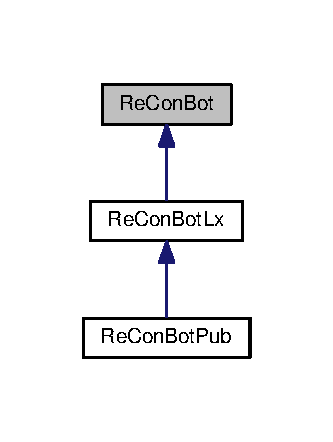
\includegraphics[width=160pt]{d5/d0d/class_re_con_bot__inherit__graph}
\end{center}
\end{figure}
\subsection*{Public Member Functions}
\begin{DoxyCompactItemize}
\item 
\hyperlink{class_re_con_bot_a3c0174965242ba69f252e09d18ce2e98}{Re\+Con\+Bot} ()
\item 
void \hyperlink{class_re_con_bot_ab859fa96532995d3c1545aaa9db1802e}{traj\+Client} ()
\item 
void \hyperlink{class_re_con_bot_ade3eb1a4752d45659321209f5730cef3}{start\+Trajectory} (control\+\_\+msgs\+::\+Follow\+Joint\+Trajectory\+Goal \hyperlink{class_re_con_bot_a9bd1c7ddf2376e2e68ea5d8bd8c3f505}{goal})
\item 
control\+\_\+msgs\+::\+Follow\+Joint\+Trajectory\+Goal \hyperlink{class_re_con_bot_a950f2769ca61ff7b663d86ed2cf19c14}{arm\+Trajectory} ()
\item 
bool \hyperlink{class_re_con_bot_ac264f3082203c3b2ef13b6f353476ca7}{run} ()
\item 
actionlib\+::\+Simple\+Client\+Goal\+State \hyperlink{class_re_con_bot_a3d9656755c06ded1f3b88ce05565f758}{get\+State} ()
\begin{DoxyCompactList}\small\item\em Returns the current state of the action. \end{DoxyCompactList}\end{DoxyCompactItemize}
\subsection*{Public Attributes}
\begin{DoxyCompactItemize}
\item 
std\+::string \hyperlink{class_re_con_bot_a65cf4bed9bbabd92e1265d05507e0945}{source\+File}
\item 
std\+::string \hyperlink{class_re_con_bot_a40ca07cd606988b78664c4a52fd8dc59}{name\+Space}
\item 
std\+::string \hyperlink{class_re_con_bot_a1d91d2ea8c0f16340440357906fb9ebf}{topic\+Name}
\end{DoxyCompactItemize}
\subsection*{Protected Attributes}
\begin{DoxyCompactItemize}
\item 
\hyperlink{basic__arm_8cpp_a6fb8875093261cdc69e54d3ac7d5c301}{Traj\+Client} $\ast$ \hyperlink{class_re_con_bot_a14a35ad6ca284af7db7228d7872720d1}{traj\+\_\+client\+\_\+}
\item 
control\+\_\+msgs\+::\+Follow\+Joint\+Trajectory\+Goal \hyperlink{class_re_con_bot_a9bd1c7ddf2376e2e68ea5d8bd8c3f505}{goal}
\item 
ros\+::\+Node\+Handle \hyperlink{class_re_con_bot_a37edfe9c2dbbf37894c9bf850806fdd3}{nh\+Pub}
\item 
ros\+::\+Publisher \hyperlink{class_re_con_bot_a549b7542d286b690f38b7ece8b83850b}{nh\+Pub\+\_\+pub}
\item 
int \hyperlink{class_re_con_bot_aba20d307ac1b2e6b22f96da83a0d937d}{topic\+Query}
\item 
std\+::vector$<$ double $>$ \hyperlink{class_re_con_bot_a7c59e136741800bf0734f659119aa5ee}{trajectory\+Points}
\end{DoxyCompactItemize}


\subsection{Detailed Description}
Class implemented for driving the \hyperlink{class_re_con_bot}{Re\+Con\+Bot} planning group. 

\begin{DoxyAuthor}{Author}
Jorge De La Cruz 
\end{DoxyAuthor}
\begin{DoxyVersion}{Version}
1.\+0 
\end{DoxyVersion}
\begin{DoxyDate}{Date}
February 20, 2017
\end{DoxyDate}
This class is created for hearing in the topic /wished\+\_\+path and the topic /collision\+\_\+object. With this information an avoidance proccedure is performed for Moveit. 

Definition at line 56 of file Re\+Con\+Bot.\+h.



\subsection{Constructor \& Destructor Documentation}
\mbox{\Hypertarget{class_re_con_bot_a3c0174965242ba69f252e09d18ce2e98}\label{class_re_con_bot_a3c0174965242ba69f252e09d18ce2e98}} 
\index{Re\+Con\+Bot@{Re\+Con\+Bot}!Re\+Con\+Bot@{Re\+Con\+Bot}}
\index{Re\+Con\+Bot@{Re\+Con\+Bot}!Re\+Con\+Bot@{Re\+Con\+Bot}}
\subsubsection{\texorpdfstring{Re\+Con\+Bot()}{ReConBot()}}
{\footnotesize\ttfamily Re\+Con\+Bot\+::\+Re\+Con\+Bot (\begin{DoxyParamCaption}{ }\end{DoxyParamCaption})\hspace{0.3cm}{\ttfamily [inline]}}



Definition at line 70 of file Re\+Con\+Bot.\+h.



References arm\+Trajectory(), get\+State(), run(), start\+Trajectory(), and traj\+Client().


\begin{DoxyCode}
70             \{
71   \}
\end{DoxyCode}
Here is the call graph for this function\+:\nopagebreak
\begin{figure}[H]
\begin{center}
\leavevmode
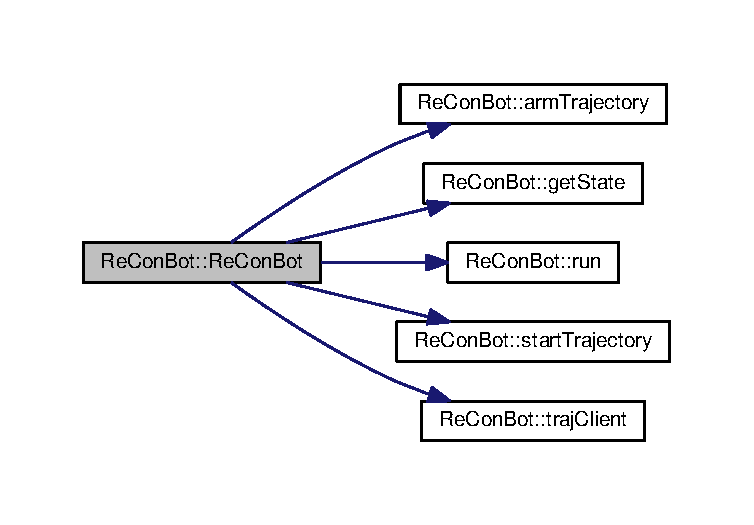
\includegraphics[width=350pt]{d9/d0b/class_re_con_bot_a3c0174965242ba69f252e09d18ce2e98_cgraph}
\end{center}
\end{figure}


\subsection{Member Function Documentation}
\mbox{\Hypertarget{class_re_con_bot_a950f2769ca61ff7b663d86ed2cf19c14}\label{class_re_con_bot_a950f2769ca61ff7b663d86ed2cf19c14}} 
\index{Re\+Con\+Bot@{Re\+Con\+Bot}!arm\+Trajectory@{arm\+Trajectory}}
\index{arm\+Trajectory@{arm\+Trajectory}!Re\+Con\+Bot@{Re\+Con\+Bot}}
\subsubsection{\texorpdfstring{arm\+Trajectory()}{armTrajectory()}}
{\footnotesize\ttfamily control\+\_\+msgs\+::\+Follow\+Joint\+Trajectory\+Goal Re\+Con\+Bot\+::arm\+Trajectory (\begin{DoxyParamCaption}{ }\end{DoxyParamCaption})}



Referenced by Re\+Con\+Bot().

Here is the caller graph for this function\+:
\nopagebreak
\begin{figure}[H]
\begin{center}
\leavevmode
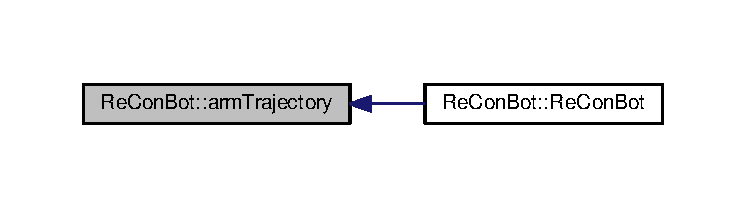
\includegraphics[width=350pt]{d9/d0b/class_re_con_bot_a950f2769ca61ff7b663d86ed2cf19c14_icgraph}
\end{center}
\end{figure}
\mbox{\Hypertarget{class_re_con_bot_a3d9656755c06ded1f3b88ce05565f758}\label{class_re_con_bot_a3d9656755c06ded1f3b88ce05565f758}} 
\index{Re\+Con\+Bot@{Re\+Con\+Bot}!get\+State@{get\+State}}
\index{get\+State@{get\+State}!Re\+Con\+Bot@{Re\+Con\+Bot}}
\subsubsection{\texorpdfstring{get\+State()}{getState()}}
{\footnotesize\ttfamily actionlib\+::\+Simple\+Client\+Goal\+State Re\+Con\+Bot\+::get\+State (\begin{DoxyParamCaption}{ }\end{DoxyParamCaption})}



Returns the current state of the action. 



Definition at line 147 of file Re\+Con\+Bot.\+h.



References traj\+\_\+client\+\_\+.



Referenced by Re\+Con\+Bot().


\begin{DoxyCode}
147                                                  \{
148   \textcolor{keywordflow}{return} \hyperlink{class_re_con_bot_a14a35ad6ca284af7db7228d7872720d1}{traj\_client\_}->getState();
149 \}
\end{DoxyCode}
Here is the caller graph for this function\+:
\nopagebreak
\begin{figure}[H]
\begin{center}
\leavevmode
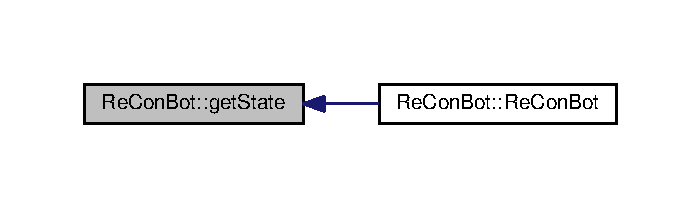
\includegraphics[width=336pt]{d9/d0b/class_re_con_bot_a3d9656755c06ded1f3b88ce05565f758_icgraph}
\end{center}
\end{figure}
\mbox{\Hypertarget{class_re_con_bot_ac264f3082203c3b2ef13b6f353476ca7}\label{class_re_con_bot_ac264f3082203c3b2ef13b6f353476ca7}} 
\index{Re\+Con\+Bot@{Re\+Con\+Bot}!run@{run}}
\index{run@{run}!Re\+Con\+Bot@{Re\+Con\+Bot}}
\subsubsection{\texorpdfstring{run()}{run()}}
{\footnotesize\ttfamily bool Re\+Con\+Bot\+::run (\begin{DoxyParamCaption}{ }\end{DoxyParamCaption})}

$<$Two spinner are instantiated for managing 2 threats 

Definition at line 118 of file Re\+Con\+Bot.\+h.



Referenced by Re\+Con\+Bot().


\begin{DoxyCode}
118                   \{
119     ros::AsyncSpinner spinner(2);
120     spinner.start();
121     ros::waitForShutdown();
122 \}
\end{DoxyCode}
Here is the caller graph for this function\+:
\nopagebreak
\begin{figure}[H]
\begin{center}
\leavevmode
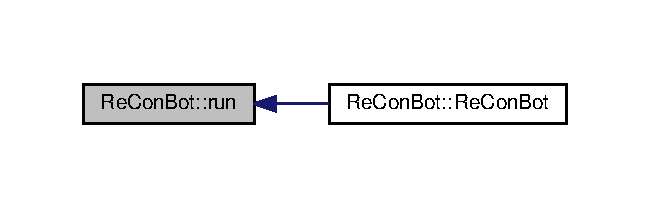
\includegraphics[width=312pt]{d9/d0b/class_re_con_bot_ac264f3082203c3b2ef13b6f353476ca7_icgraph}
\end{center}
\end{figure}
\mbox{\Hypertarget{class_re_con_bot_ade3eb1a4752d45659321209f5730cef3}\label{class_re_con_bot_ade3eb1a4752d45659321209f5730cef3}} 
\index{Re\+Con\+Bot@{Re\+Con\+Bot}!start\+Trajectory@{start\+Trajectory}}
\index{start\+Trajectory@{start\+Trajectory}!Re\+Con\+Bot@{Re\+Con\+Bot}}
\subsubsection{\texorpdfstring{start\+Trajectory()}{startTrajectory()}}
{\footnotesize\ttfamily void Re\+Con\+Bot\+::start\+Trajectory (\begin{DoxyParamCaption}\item[{control\+\_\+msgs\+::\+Follow\+Joint\+Trajectory\+Goal}]{goal }\end{DoxyParamCaption})}

Sends the command to start a given trajectory 

Definition at line 127 of file Re\+Con\+Bot.\+h.



References traj\+\_\+client\+\_\+.



Referenced by Re\+Con\+Bot(), and Re\+Con\+Bot\+Lx\+::reconbot\+Callback().


\begin{DoxyCode}
127                                                                         \{
128   ROS\_INFO(\textcolor{stringliteral}{"=========== Welcome to IGM - ReConBot Move Group Interface =============="});
129   ROS\_INFO(\textcolor{stringliteral}{"=========== Group of Robotic and Mechatronic               =============="});
130 
131     \textcolor{comment}{// When to start the trajectory: 1s from now}
132     \hyperlink{class_re_con_bot_a9bd1c7ddf2376e2e68ea5d8bd8c3f505}{goal}.trajectory.header.stamp = ros::Time::now() + ros::Duration(1.0);
133     \hyperlink{class_re_con_bot_a14a35ad6ca284af7db7228d7872720d1}{traj\_client\_}->sendGoal(\hyperlink{class_re_con_bot_a9bd1c7ddf2376e2e68ea5d8bd8c3f505}{goal});
134   \}
\end{DoxyCode}
Here is the caller graph for this function\+:
\nopagebreak
\begin{figure}[H]
\begin{center}
\leavevmode
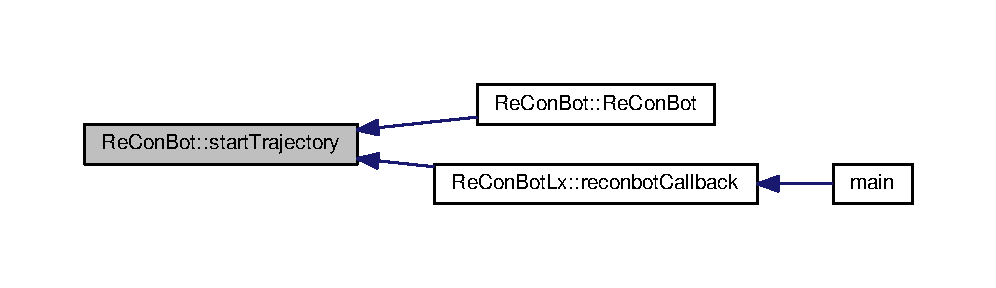
\includegraphics[width=350pt]{d9/d0b/class_re_con_bot_ade3eb1a4752d45659321209f5730cef3_icgraph}
\end{center}
\end{figure}
\mbox{\Hypertarget{class_re_con_bot_ab859fa96532995d3c1545aaa9db1802e}\label{class_re_con_bot_ab859fa96532995d3c1545aaa9db1802e}} 
\index{Re\+Con\+Bot@{Re\+Con\+Bot}!traj\+Client@{traj\+Client}}
\index{traj\+Client@{traj\+Client}!Re\+Con\+Bot@{Re\+Con\+Bot}}
\subsubsection{\texorpdfstring{traj\+Client()}{trajClient()}}
{\footnotesize\ttfamily void Re\+Con\+Bot\+::traj\+Client (\begin{DoxyParamCaption}{ }\end{DoxyParamCaption})}

tell the action client that we want to spin a thread by default

Definition at line 106 of file Re\+Con\+Bot.\+h.



References name\+Space, and traj\+\_\+client\+\_\+.



Referenced by main(), and Re\+Con\+Bot().


\begin{DoxyCode}
106                          \{
110   \hyperlink{class_re_con_bot_a14a35ad6ca284af7db7228d7872720d1}{traj\_client\_} = \textcolor{keyword}{new} \hyperlink{_re_con_bot_8h_a6fb8875093261cdc69e54d3ac7d5c301}{TrajClient}(\hyperlink{class_re_con_bot_a40ca07cd606988b78664c4a52fd8dc59}{nameSpace} + \textcolor{stringliteral}{"/follow\_joint\_trajectory"}, \textcolor{keyword}{true}
      );
111 
112   \textcolor{comment}{// wait for action server to come up}
113   \textcolor{keywordflow}{while}(!\hyperlink{class_re_con_bot_a14a35ad6ca284af7db7228d7872720d1}{traj\_client\_}->waitForServer(ros::Duration(5.0)))\{
114   ROS\_INFO(\textcolor{stringliteral}{"Waiting for the joint\_trajectory\_action server"});
115   \}
116 \}
\end{DoxyCode}
Here is the caller graph for this function\+:
\nopagebreak
\begin{figure}[H]
\begin{center}
\leavevmode
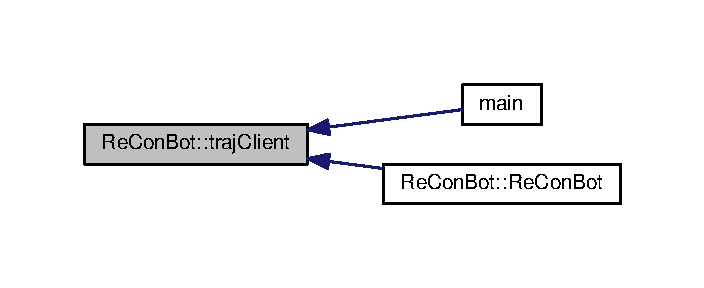
\includegraphics[width=338pt]{d9/d0b/class_re_con_bot_ab859fa96532995d3c1545aaa9db1802e_icgraph}
\end{center}
\end{figure}


\subsection{Member Data Documentation}
\mbox{\Hypertarget{class_re_con_bot_a9bd1c7ddf2376e2e68ea5d8bd8c3f505}\label{class_re_con_bot_a9bd1c7ddf2376e2e68ea5d8bd8c3f505}} 
\index{Re\+Con\+Bot@{Re\+Con\+Bot}!goal@{goal}}
\index{goal@{goal}!Re\+Con\+Bot@{Re\+Con\+Bot}}
\subsubsection{\texorpdfstring{goal}{goal}}
{\footnotesize\ttfamily control\+\_\+msgs\+::\+Follow\+Joint\+Trajectory\+Goal Re\+Con\+Bot\+::goal\hspace{0.3cm}{\ttfamily [protected]}}



Definition at line 60 of file Re\+Con\+Bot.\+h.



Referenced by Re\+Con\+Bot\+Pub\+::build\+Trajectory(), Re\+Con\+Bot\+Lx\+::\+Re\+Con\+Bot\+Lx(), and Re\+Con\+Bot\+Pub\+::\+Re\+Con\+Bot\+Pub().

\mbox{\Hypertarget{class_re_con_bot_a40ca07cd606988b78664c4a52fd8dc59}\label{class_re_con_bot_a40ca07cd606988b78664c4a52fd8dc59}} 
\index{Re\+Con\+Bot@{Re\+Con\+Bot}!name\+Space@{name\+Space}}
\index{name\+Space@{name\+Space}!Re\+Con\+Bot@{Re\+Con\+Bot}}
\subsubsection{\texorpdfstring{name\+Space}{nameSpace}}
{\footnotesize\ttfamily std\+::string Re\+Con\+Bot\+::name\+Space}



Definition at line 68 of file Re\+Con\+Bot.\+h.



Referenced by main(), and traj\+Client().

\mbox{\Hypertarget{class_re_con_bot_a37edfe9c2dbbf37894c9bf850806fdd3}\label{class_re_con_bot_a37edfe9c2dbbf37894c9bf850806fdd3}} 
\index{Re\+Con\+Bot@{Re\+Con\+Bot}!nh\+Pub@{nh\+Pub}}
\index{nh\+Pub@{nh\+Pub}!Re\+Con\+Bot@{Re\+Con\+Bot}}
\subsubsection{\texorpdfstring{nh\+Pub}{nhPub}}
{\footnotesize\ttfamily ros\+::\+Node\+Handle Re\+Con\+Bot\+::nh\+Pub\hspace{0.3cm}{\ttfamily [protected]}}



Definition at line 61 of file Re\+Con\+Bot.\+h.



Referenced by Re\+Con\+Bot\+Pub\+::trajectory\+Publisher\+Start().

\mbox{\Hypertarget{class_re_con_bot_a549b7542d286b690f38b7ece8b83850b}\label{class_re_con_bot_a549b7542d286b690f38b7ece8b83850b}} 
\index{Re\+Con\+Bot@{Re\+Con\+Bot}!nh\+Pub\+\_\+pub@{nh\+Pub\+\_\+pub}}
\index{nh\+Pub\+\_\+pub@{nh\+Pub\+\_\+pub}!Re\+Con\+Bot@{Re\+Con\+Bot}}
\subsubsection{\texorpdfstring{nh\+Pub\+\_\+pub}{nhPub\_pub}}
{\footnotesize\ttfamily ros\+::\+Publisher Re\+Con\+Bot\+::nh\+Pub\+\_\+pub\hspace{0.3cm}{\ttfamily [protected]}}



Definition at line 62 of file Re\+Con\+Bot.\+h.



Referenced by Re\+Con\+Bot\+Pub\+::publisher(), and Re\+Con\+Bot\+Pub\+::trajectory\+Publisher\+Start().

\mbox{\Hypertarget{class_re_con_bot_a65cf4bed9bbabd92e1265d05507e0945}\label{class_re_con_bot_a65cf4bed9bbabd92e1265d05507e0945}} 
\index{Re\+Con\+Bot@{Re\+Con\+Bot}!source\+File@{source\+File}}
\index{source\+File@{source\+File}!Re\+Con\+Bot@{Re\+Con\+Bot}}
\subsubsection{\texorpdfstring{source\+File}{sourceFile}}
{\footnotesize\ttfamily std\+::string Re\+Con\+Bot\+::source\+File}

File directory with pose data 

Definition at line 67 of file Re\+Con\+Bot.\+h.



Referenced by Re\+Con\+Bot\+Pub\+::build\+Trajectory(), main(), and Re\+Con\+Bot\+Pub\+::\+Re\+Con\+Bot\+Pub().

\mbox{\Hypertarget{class_re_con_bot_a1d91d2ea8c0f16340440357906fb9ebf}\label{class_re_con_bot_a1d91d2ea8c0f16340440357906fb9ebf}} 
\index{Re\+Con\+Bot@{Re\+Con\+Bot}!topic\+Name@{topic\+Name}}
\index{topic\+Name@{topic\+Name}!Re\+Con\+Bot@{Re\+Con\+Bot}}
\subsubsection{\texorpdfstring{topic\+Name}{topicName}}
{\footnotesize\ttfamily std\+::string Re\+Con\+Bot\+::topic\+Name}

Name given to the topic where is publishing. 

Definition at line 69 of file Re\+Con\+Bot.\+h.



Referenced by main(), Re\+Con\+Bot\+Pub\+::\+Re\+Con\+Bot\+Pub(), and Re\+Con\+Bot\+Pub\+::trajectory\+Publisher\+Start().

\mbox{\Hypertarget{class_re_con_bot_aba20d307ac1b2e6b22f96da83a0d937d}\label{class_re_con_bot_aba20d307ac1b2e6b22f96da83a0d937d}} 
\index{Re\+Con\+Bot@{Re\+Con\+Bot}!topic\+Query@{topic\+Query}}
\index{topic\+Query@{topic\+Query}!Re\+Con\+Bot@{Re\+Con\+Bot}}
\subsubsection{\texorpdfstring{topic\+Query}{topicQuery}}
{\footnotesize\ttfamily int Re\+Con\+Bot\+::topic\+Query\hspace{0.3cm}{\ttfamily [protected]}}



Definition at line 63 of file Re\+Con\+Bot.\+h.



Referenced by Re\+Con\+Bot\+Pub\+::\+Re\+Con\+Bot\+Pub(), and Re\+Con\+Bot\+Pub\+::trajectory\+Publisher\+Start().

\mbox{\Hypertarget{class_re_con_bot_a14a35ad6ca284af7db7228d7872720d1}\label{class_re_con_bot_a14a35ad6ca284af7db7228d7872720d1}} 
\index{Re\+Con\+Bot@{Re\+Con\+Bot}!traj\+\_\+client\+\_\+@{traj\+\_\+client\+\_\+}}
\index{traj\+\_\+client\+\_\+@{traj\+\_\+client\+\_\+}!Re\+Con\+Bot@{Re\+Con\+Bot}}
\subsubsection{\texorpdfstring{traj\+\_\+client\+\_\+}{traj\_client\_}}
{\footnotesize\ttfamily \hyperlink{basic__arm_8cpp_a6fb8875093261cdc69e54d3ac7d5c301}{Traj\+Client}$\ast$ Re\+Con\+Bot\+::traj\+\_\+client\+\_\+\hspace{0.3cm}{\ttfamily [protected]}}



Definition at line 59 of file Re\+Con\+Bot.\+h.



Referenced by get\+State(), start\+Trajectory(), and traj\+Client().

\mbox{\Hypertarget{class_re_con_bot_a7c59e136741800bf0734f659119aa5ee}\label{class_re_con_bot_a7c59e136741800bf0734f659119aa5ee}} 
\index{Re\+Con\+Bot@{Re\+Con\+Bot}!trajectory\+Points@{trajectory\+Points}}
\index{trajectory\+Points@{trajectory\+Points}!Re\+Con\+Bot@{Re\+Con\+Bot}}
\subsubsection{\texorpdfstring{trajectory\+Points}{trajectoryPoints}}
{\footnotesize\ttfamily std\+::vector$<$double$>$ Re\+Con\+Bot\+::trajectory\+Points\hspace{0.3cm}{\ttfamily [protected]}}



Definition at line 64 of file Re\+Con\+Bot.\+h.



Referenced by Re\+Con\+Bot\+Pub\+::build\+Trajectory().



The documentation for this class was generated from the following file\+:\begin{DoxyCompactItemize}
\item 
\hyperlink{_re_con_bot_8h}{Re\+Con\+Bot.\+h}\end{DoxyCompactItemize}

\hypertarget{class_re_con_bot_arm}{}\section{Re\+Con\+Bot\+Arm Class Reference}
\label{class_re_con_bot_arm}\index{Re\+Con\+Bot\+Arm@{Re\+Con\+Bot\+Arm}}
\subsection*{Public Member Functions}
\begin{DoxyCompactItemize}
\item 
\hyperlink{class_re_con_bot_arm_acdc750bbe5edac6d78c117e0b2073c60}{Re\+Con\+Bot\+Arm} ()
\item 
\hyperlink{class_re_con_bot_arm_ab8ce7d41fb625ac7ad8486278b5e2a45}{$\sim$\+Re\+Con\+Bot\+Arm} ()
\begin{DoxyCompactList}\small\item\em Clean up the action client. \end{DoxyCompactList}\item 
void \hyperlink{class_re_con_bot_arm_a52f6f89615b17a421d5cd8b51b2962d7}{start\+Trajectory} (control\+\_\+msgs\+::\+Follow\+Joint\+Trajectory\+Goal goal)
\begin{DoxyCompactList}\small\item\em Sends the command to start a given trajectory. \end{DoxyCompactList}\item 
control\+\_\+msgs\+::\+Follow\+Joint\+Trajectory\+Goal \hyperlink{class_re_con_bot_arm_ac499ee22d73b90c860f06a16afcd2fb0}{arm\+Trajectory} ()
\item 
actionlib\+::\+Simple\+Client\+Goal\+State \hyperlink{class_re_con_bot_arm_a179480efa62ff256fb8b3ddc0685d762}{get\+State} ()
\begin{DoxyCompactList}\small\item\em Returns the current state of the action. \end{DoxyCompactList}\end{DoxyCompactItemize}
\subsection*{Private Attributes}
\begin{DoxyCompactItemize}
\item 
\hyperlink{basic__arm_8cpp_a6fb8875093261cdc69e54d3ac7d5c301}{Traj\+Client} $\ast$ \hyperlink{class_re_con_bot_arm_a0be83821f776c5ca9874fabbeaa177cf}{traj\+\_\+client\+\_\+}
\end{DoxyCompactItemize}


\subsection{Detailed Description}


Definition at line 47 of file basic\+\_\+arm.\+cpp.



\subsection{Constructor \& Destructor Documentation}
\mbox{\Hypertarget{class_re_con_bot_arm_acdc750bbe5edac6d78c117e0b2073c60}\label{class_re_con_bot_arm_acdc750bbe5edac6d78c117e0b2073c60}} 
\index{Re\+Con\+Bot\+Arm@{Re\+Con\+Bot\+Arm}!Re\+Con\+Bot\+Arm@{Re\+Con\+Bot\+Arm}}
\index{Re\+Con\+Bot\+Arm@{Re\+Con\+Bot\+Arm}!Re\+Con\+Bot\+Arm@{Re\+Con\+Bot\+Arm}}
\subsubsection{\texorpdfstring{Re\+Con\+Bot\+Arm()}{ReConBotArm()}}
{\footnotesize\ttfamily Re\+Con\+Bot\+Arm\+::\+Re\+Con\+Bot\+Arm (\begin{DoxyParamCaption}{ }\end{DoxyParamCaption})\hspace{0.3cm}{\ttfamily [inline]}}



Definition at line 52 of file basic\+\_\+arm.\+cpp.


\begin{DoxyCode}
53   \{
54     \textcolor{comment}{// tell the action client that we want to spin a thread by default}
55     \hyperlink{class_re_con_bot_arm_a0be83821f776c5ca9874fabbeaa177cf}{traj\_client\_} = \textcolor{keyword}{new} \hyperlink{basic__arm_8cpp_a6fb8875093261cdc69e54d3ac7d5c301}{TrajClient}(\textcolor{stringliteral}{"reconbot\_arm\_controller/follow\_joint\_trajectory"}, \textcolor{keyword}{
      true});
56 
57     \textcolor{comment}{// wait for action server to come up}
58     \textcolor{keywordflow}{while}(!\hyperlink{class_re_con_bot_arm_a0be83821f776c5ca9874fabbeaa177cf}{traj\_client\_}->waitForServer(ros::Duration(5.0)))\{
59     ROS\_INFO(\textcolor{stringliteral}{"Waiting for the joint\_trajectory\_action server"});
60     \}
61   \}
\end{DoxyCode}
\mbox{\Hypertarget{class_re_con_bot_arm_ab8ce7d41fb625ac7ad8486278b5e2a45}\label{class_re_con_bot_arm_ab8ce7d41fb625ac7ad8486278b5e2a45}} 
\index{Re\+Con\+Bot\+Arm@{Re\+Con\+Bot\+Arm}!````~Re\+Con\+Bot\+Arm@{$\sim$\+Re\+Con\+Bot\+Arm}}
\index{````~Re\+Con\+Bot\+Arm@{$\sim$\+Re\+Con\+Bot\+Arm}!Re\+Con\+Bot\+Arm@{Re\+Con\+Bot\+Arm}}
\subsubsection{\texorpdfstring{$\sim$\+Re\+Con\+Bot\+Arm()}{~ReConBotArm()}}
{\footnotesize\ttfamily Re\+Con\+Bot\+Arm\+::$\sim$\+Re\+Con\+Bot\+Arm (\begin{DoxyParamCaption}{ }\end{DoxyParamCaption})\hspace{0.3cm}{\ttfamily [inline]}}



Clean up the action client. 



Definition at line 63 of file basic\+\_\+arm.\+cpp.



References traj\+\_\+client\+\_\+.


\begin{DoxyCode}
64   \{
65   \textcolor{keyword}{delete} \hyperlink{class_re_con_bot_arm_a0be83821f776c5ca9874fabbeaa177cf}{traj\_client\_};
66   \}
\end{DoxyCode}


\subsection{Member Function Documentation}
\mbox{\Hypertarget{class_re_con_bot_arm_ac499ee22d73b90c860f06a16afcd2fb0}\label{class_re_con_bot_arm_ac499ee22d73b90c860f06a16afcd2fb0}} 
\index{Re\+Con\+Bot\+Arm@{Re\+Con\+Bot\+Arm}!arm\+Trajectory@{arm\+Trajectory}}
\index{arm\+Trajectory@{arm\+Trajectory}!Re\+Con\+Bot\+Arm@{Re\+Con\+Bot\+Arm}}
\subsubsection{\texorpdfstring{arm\+Trajectory()}{armTrajectory()}}
{\footnotesize\ttfamily control\+\_\+msgs\+::\+Follow\+Joint\+Trajectory\+Goal Re\+Con\+Bot\+Arm\+::arm\+Trajectory (\begin{DoxyParamCaption}{ }\end{DoxyParamCaption})\hspace{0.3cm}{\ttfamily [inline]}}



Definition at line 76 of file basic\+\_\+arm.\+cpp.



Referenced by main().


\begin{DoxyCode}
77     \{
78       \textcolor{comment}{//our goal variable}
79       control\_msgs::FollowJointTrajectoryGoal goal;
80 
81       \textcolor{comment}{// First, the joint names, which apply to all waypoints}
82       goal.trajectory.joint\_names.push\_back(\textcolor{stringliteral}{"joint\_1"});
83       goal.trajectory.joint\_names.push\_back(\textcolor{stringliteral}{"joint\_2"});
84       goal.trajectory.joint\_names.push\_back(\textcolor{stringliteral}{"joint\_3"});
85 
86       \textcolor{comment}{// We will have two waypoints in this goal trajectory}
87       goal.trajectory.points.resize(3);
88 
89       \textcolor{comment}{// First trajectory point}
90       \textcolor{comment}{// Positions}
91       \textcolor{keywordtype}{int} ind = 0;
92       goal.trajectory.points[ind].positions.resize(3);
93       goal.trajectory.points[ind].positions[0] = 0.0;
94       goal.trajectory.points[ind].positions[1] = 0.0;
95       goal.trajectory.points[ind].positions[2] = 0.4363;
96       \textcolor{comment}{// Velocities}
97       goal.trajectory.points[ind].velocities.resize(3);
98       \textcolor{keywordflow}{for} (\textcolor{keywordtype}{size\_t} j = 0; j < 3; ++j)
99       \{
100         goal.trajectory.points[ind].velocities[j] = 0.0;
101       \}
102       \textcolor{comment}{// To be reached 1 second after starting along the trajectory}
103       goal.trajectory.points[ind].time\_from\_start = ros::Duration(2.0);
104 
105       \textcolor{comment}{// Second trajectory point}
106       \textcolor{comment}{// Positions}
107       ind = 1;
108       goal.trajectory.points[ind].positions.resize(3);
109       goal.trajectory.points[ind].positions[0] = 1.5708;
110       goal.trajectory.points[ind].positions[1] = 1.5708;
111       goal.trajectory.points[ind].positions[2] = 3.5779;
112       \textcolor{comment}{// Velocities}
113       goal.trajectory.points[ind].velocities.resize(3);
114       \textcolor{keywordflow}{for} (\textcolor{keywordtype}{size\_t} j = 0; j < 3; ++j)
115       \{
116         goal.trajectory.points[ind].velocities[j] = 0.0;
117       \}
118       \textcolor{comment}{// To be reached 2 seconds after starting along the trajectory}
119       goal.trajectory.points[ind].time\_from\_start = ros::Duration(4.0);
120 
121       ind = 2;
122       goal.trajectory.points[ind].positions.resize(3);
123       goal.trajectory.points[ind].positions[0] = 0.0;
124       goal.trajectory.points[ind].positions[1] = 0.0;
125       goal.trajectory.points[ind].positions[2] = 0.4363;
126       \textcolor{comment}{// Velocities}
127       goal.trajectory.points[ind].velocities.resize(3);
128       \textcolor{keywordflow}{for} (\textcolor{keywordtype}{size\_t} j = 0; j < 3; ++j)
129       \{
130         goal.trajectory.points[ind].velocities[j] = 0.0;
131       \}
132       \textcolor{comment}{// To be reached 2 seconds after starting along the trajectory}
133       goal.trajectory.points[ind].time\_from\_start = ros::Duration(6.0);
134 
135       \textcolor{comment}{//we are done; return the goal}
136       \textcolor{keywordflow}{return} goal;
137     \}
\end{DoxyCode}
Here is the caller graph for this function\+:\nopagebreak
\begin{figure}[H]
\begin{center}
\leavevmode
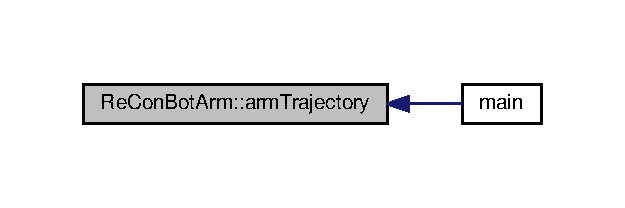
\includegraphics[width=300pt]{d3/d06/class_re_con_bot_arm_ac499ee22d73b90c860f06a16afcd2fb0_icgraph}
\end{center}
\end{figure}
\mbox{\Hypertarget{class_re_con_bot_arm_a179480efa62ff256fb8b3ddc0685d762}\label{class_re_con_bot_arm_a179480efa62ff256fb8b3ddc0685d762}} 
\index{Re\+Con\+Bot\+Arm@{Re\+Con\+Bot\+Arm}!get\+State@{get\+State}}
\index{get\+State@{get\+State}!Re\+Con\+Bot\+Arm@{Re\+Con\+Bot\+Arm}}
\subsubsection{\texorpdfstring{get\+State()}{getState()}}
{\footnotesize\ttfamily actionlib\+::\+Simple\+Client\+Goal\+State Re\+Con\+Bot\+Arm\+::get\+State (\begin{DoxyParamCaption}{ }\end{DoxyParamCaption})\hspace{0.3cm}{\ttfamily [inline]}}



Returns the current state of the action. 



Definition at line 140 of file basic\+\_\+arm.\+cpp.



Referenced by main().


\begin{DoxyCode}
141     \{
142       \textcolor{keywordflow}{return} \hyperlink{class_re_con_bot_arm_a0be83821f776c5ca9874fabbeaa177cf}{traj\_client\_}->getState();
143     \}
\end{DoxyCode}
Here is the caller graph for this function\+:\nopagebreak
\begin{figure}[H]
\begin{center}
\leavevmode
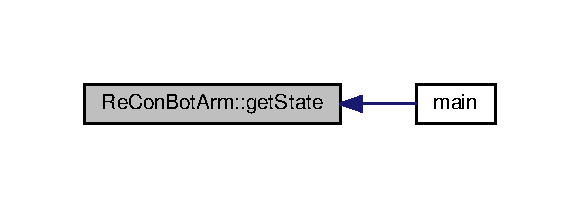
\includegraphics[width=278pt]{d3/d06/class_re_con_bot_arm_a179480efa62ff256fb8b3ddc0685d762_icgraph}
\end{center}
\end{figure}
\mbox{\Hypertarget{class_re_con_bot_arm_a52f6f89615b17a421d5cd8b51b2962d7}\label{class_re_con_bot_arm_a52f6f89615b17a421d5cd8b51b2962d7}} 
\index{Re\+Con\+Bot\+Arm@{Re\+Con\+Bot\+Arm}!start\+Trajectory@{start\+Trajectory}}
\index{start\+Trajectory@{start\+Trajectory}!Re\+Con\+Bot\+Arm@{Re\+Con\+Bot\+Arm}}
\subsubsection{\texorpdfstring{start\+Trajectory()}{startTrajectory()}}
{\footnotesize\ttfamily void Re\+Con\+Bot\+Arm\+::start\+Trajectory (\begin{DoxyParamCaption}\item[{control\+\_\+msgs\+::\+Follow\+Joint\+Trajectory\+Goal}]{goal }\end{DoxyParamCaption})\hspace{0.3cm}{\ttfamily [inline]}}



Sends the command to start a given trajectory. 



Definition at line 68 of file basic\+\_\+arm.\+cpp.



Referenced by main().


\begin{DoxyCode}
69     \{
70       \textcolor{comment}{// When to start the trajectory: 1s from now}
71       goal.trajectory.header.stamp = ros::Time::now() + ros::Duration(1.0);
72       \hyperlink{class_re_con_bot_arm_a0be83821f776c5ca9874fabbeaa177cf}{traj\_client\_}->sendGoal(goal);
73     \}
\end{DoxyCode}
Here is the caller graph for this function\+:\nopagebreak
\begin{figure}[H]
\begin{center}
\leavevmode
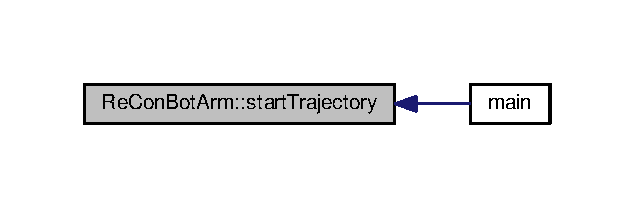
\includegraphics[width=304pt]{d3/d06/class_re_con_bot_arm_a52f6f89615b17a421d5cd8b51b2962d7_icgraph}
\end{center}
\end{figure}


\subsection{Member Data Documentation}
\mbox{\Hypertarget{class_re_con_bot_arm_a0be83821f776c5ca9874fabbeaa177cf}\label{class_re_con_bot_arm_a0be83821f776c5ca9874fabbeaa177cf}} 
\index{Re\+Con\+Bot\+Arm@{Re\+Con\+Bot\+Arm}!traj\+\_\+client\+\_\+@{traj\+\_\+client\+\_\+}}
\index{traj\+\_\+client\+\_\+@{traj\+\_\+client\+\_\+}!Re\+Con\+Bot\+Arm@{Re\+Con\+Bot\+Arm}}
\subsubsection{\texorpdfstring{traj\+\_\+client\+\_\+}{traj\_client\_}}
{\footnotesize\ttfamily \hyperlink{basic__arm_8cpp_a6fb8875093261cdc69e54d3ac7d5c301}{Traj\+Client}$\ast$ Re\+Con\+Bot\+Arm\+::traj\+\_\+client\+\_\+\hspace{0.3cm}{\ttfamily [private]}}



Definition at line 50 of file basic\+\_\+arm.\+cpp.



Referenced by $\sim$\+Re\+Con\+Bot\+Arm().



The documentation for this class was generated from the following file\+:\begin{DoxyCompactItemize}
\item 
\hyperlink{basic__arm_8cpp}{basic\+\_\+arm.\+cpp}\end{DoxyCompactItemize}

\hypertarget{class_re_con_bot_lx}{}\section{Re\+Con\+Bot\+Lx Class Reference}
\label{class_re_con_bot_lx}\index{Re\+Con\+Bot\+Lx@{Re\+Con\+Bot\+Lx}}


{\ttfamily \#include $<$Re\+Con\+Bot.\+h$>$}



Inheritance diagram for Re\+Con\+Bot\+Lx\+:\nopagebreak
\begin{figure}[H]
\begin{center}
\leavevmode
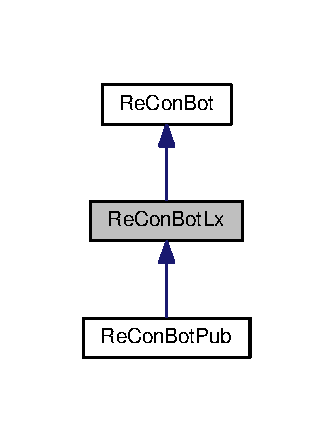
\includegraphics[width=160pt]{dc/db8/class_re_con_bot_lx__inherit__graph}
\end{center}
\end{figure}


Collaboration diagram for Re\+Con\+Bot\+Lx\+:\nopagebreak
\begin{figure}[H]
\begin{center}
\leavevmode
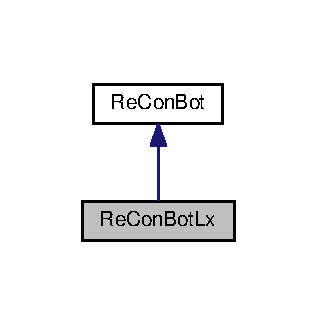
\includegraphics[width=152pt]{d3/dfa/class_re_con_bot_lx__coll__graph}
\end{center}
\end{figure}
\subsection*{Public Member Functions}
\begin{DoxyCompactItemize}
\item 
\hyperlink{class_re_con_bot_lx_aa4c8b9071629aceec362d46287da4984}{Re\+Con\+Bot\+Lx} ()
\item 
void \hyperlink{class_re_con_bot_lx_a0e25f573057755c6729ea572362652e6}{motors\+State} (int arg\mbox{[}$\,$\mbox{]}, int length)
\item 
void \hyperlink{class_re_con_bot_lx_a5d60b16962e5ce8e452f7c53543c54ce}{reconbot\+Callback} (const control\+\_\+msgs\+::\+Follow\+Joint\+Trajectory\+Goal \hyperlink{class_re_con_bot_a9bd1c7ddf2376e2e68ea5d8bd8c3f505}{goal})
\item 
void \hyperlink{class_re_con_bot_ab859fa96532995d3c1545aaa9db1802e}{traj\+Client} ()
\item 
void \hyperlink{class_re_con_bot_ade3eb1a4752d45659321209f5730cef3}{start\+Trajectory} (control\+\_\+msgs\+::\+Follow\+Joint\+Trajectory\+Goal \hyperlink{class_re_con_bot_a9bd1c7ddf2376e2e68ea5d8bd8c3f505}{goal})
\item 
control\+\_\+msgs\+::\+Follow\+Joint\+Trajectory\+Goal \hyperlink{class_re_con_bot_a950f2769ca61ff7b663d86ed2cf19c14}{arm\+Trajectory} ()
\item 
bool \hyperlink{class_re_con_bot_ac264f3082203c3b2ef13b6f353476ca7}{run} ()
\item 
actionlib\+::\+Simple\+Client\+Goal\+State \hyperlink{class_re_con_bot_a3d9656755c06ded1f3b88ce05565f758}{get\+State} ()
\begin{DoxyCompactList}\small\item\em Returns the current state of the action. \end{DoxyCompactList}\end{DoxyCompactItemize}
\subsection*{Public Attributes}
\begin{DoxyCompactItemize}
\item 
std\+::string \hyperlink{class_re_con_bot_a65cf4bed9bbabd92e1265d05507e0945}{source\+File}
\item 
std\+::string \hyperlink{class_re_con_bot_a40ca07cd606988b78664c4a52fd8dc59}{name\+Space}
\item 
std\+::string \hyperlink{class_re_con_bot_a1d91d2ea8c0f16340440357906fb9ebf}{topic\+Name}
\end{DoxyCompactItemize}
\subsection*{Protected Attributes}
\begin{DoxyCompactItemize}
\item 
\hyperlink{basic__arm_8cpp_a6fb8875093261cdc69e54d3ac7d5c301}{Traj\+Client} $\ast$ \hyperlink{class_re_con_bot_a14a35ad6ca284af7db7228d7872720d1}{traj\+\_\+client\+\_\+}
\item 
control\+\_\+msgs\+::\+Follow\+Joint\+Trajectory\+Goal \hyperlink{class_re_con_bot_a9bd1c7ddf2376e2e68ea5d8bd8c3f505}{goal}
\item 
ros\+::\+Node\+Handle \hyperlink{class_re_con_bot_a37edfe9c2dbbf37894c9bf850806fdd3}{nh\+Pub}
\item 
ros\+::\+Publisher \hyperlink{class_re_con_bot_a549b7542d286b690f38b7ece8b83850b}{nh\+Pub\+\_\+pub}
\item 
int \hyperlink{class_re_con_bot_aba20d307ac1b2e6b22f96da83a0d937d}{topic\+Query}
\item 
std\+::vector$<$ double $>$ \hyperlink{class_re_con_bot_a7c59e136741800bf0734f659119aa5ee}{trajectory\+Points}
\end{DoxyCompactItemize}


\subsection{Detailed Description}


Definition at line 80 of file Re\+Con\+Bot.\+h.



\subsection{Constructor \& Destructor Documentation}
\mbox{\Hypertarget{class_re_con_bot_lx_aa4c8b9071629aceec362d46287da4984}\label{class_re_con_bot_lx_aa4c8b9071629aceec362d46287da4984}} 
\index{Re\+Con\+Bot\+Lx@{Re\+Con\+Bot\+Lx}!Re\+Con\+Bot\+Lx@{Re\+Con\+Bot\+Lx}}
\index{Re\+Con\+Bot\+Lx@{Re\+Con\+Bot\+Lx}!Re\+Con\+Bot\+Lx@{Re\+Con\+Bot\+Lx}}
\subsubsection{\texorpdfstring{Re\+Con\+Bot\+Lx()}{ReConBotLx()}}
{\footnotesize\ttfamily Re\+Con\+Bot\+Lx\+::\+Re\+Con\+Bot\+Lx (\begin{DoxyParamCaption}{ }\end{DoxyParamCaption})\hspace{0.3cm}{\ttfamily [inline]}}



Definition at line 82 of file Re\+Con\+Bot.\+h.



References Re\+Con\+Bot\+::goal.


\begin{DoxyCode}
82               \{
83   \}
\end{DoxyCode}


\subsection{Member Function Documentation}
\mbox{\Hypertarget{class_re_con_bot_a950f2769ca61ff7b663d86ed2cf19c14}\label{class_re_con_bot_a950f2769ca61ff7b663d86ed2cf19c14}} 
\index{Re\+Con\+Bot\+Lx@{Re\+Con\+Bot\+Lx}!arm\+Trajectory@{arm\+Trajectory}}
\index{arm\+Trajectory@{arm\+Trajectory}!Re\+Con\+Bot\+Lx@{Re\+Con\+Bot\+Lx}}
\subsubsection{\texorpdfstring{arm\+Trajectory()}{armTrajectory()}}
{\footnotesize\ttfamily control\+\_\+msgs\+::\+Follow\+Joint\+Trajectory\+Goal Re\+Con\+Bot\+::arm\+Trajectory (\begin{DoxyParamCaption}{ }\end{DoxyParamCaption})\hspace{0.3cm}{\ttfamily [inherited]}}



Referenced by Re\+Con\+Bot\+::\+Re\+Con\+Bot().

Here is the caller graph for this function\+:
\nopagebreak
\begin{figure}[H]
\begin{center}
\leavevmode
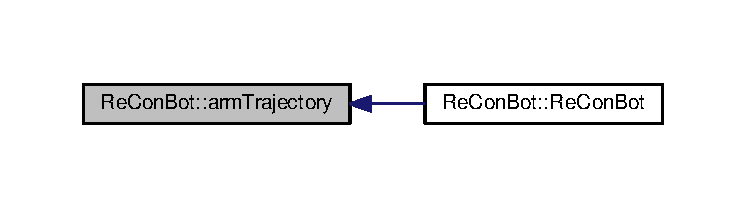
\includegraphics[width=350pt]{d9/d0b/class_re_con_bot_a950f2769ca61ff7b663d86ed2cf19c14_icgraph}
\end{center}
\end{figure}
\mbox{\Hypertarget{class_re_con_bot_a3d9656755c06ded1f3b88ce05565f758}\label{class_re_con_bot_a3d9656755c06ded1f3b88ce05565f758}} 
\index{Re\+Con\+Bot\+Lx@{Re\+Con\+Bot\+Lx}!get\+State@{get\+State}}
\index{get\+State@{get\+State}!Re\+Con\+Bot\+Lx@{Re\+Con\+Bot\+Lx}}
\subsubsection{\texorpdfstring{get\+State()}{getState()}}
{\footnotesize\ttfamily actionlib\+::\+Simple\+Client\+Goal\+State Re\+Con\+Bot\+::get\+State (\begin{DoxyParamCaption}{ }\end{DoxyParamCaption})\hspace{0.3cm}{\ttfamily [inherited]}}



Returns the current state of the action. 



Definition at line 147 of file Re\+Con\+Bot.\+h.



References Re\+Con\+Bot\+::traj\+\_\+client\+\_\+.



Referenced by Re\+Con\+Bot\+::\+Re\+Con\+Bot().


\begin{DoxyCode}
147                                                  \{
148   \textcolor{keywordflow}{return} \hyperlink{class_re_con_bot_a14a35ad6ca284af7db7228d7872720d1}{traj\_client\_}->getState();
149 \}
\end{DoxyCode}
Here is the caller graph for this function\+:
\nopagebreak
\begin{figure}[H]
\begin{center}
\leavevmode
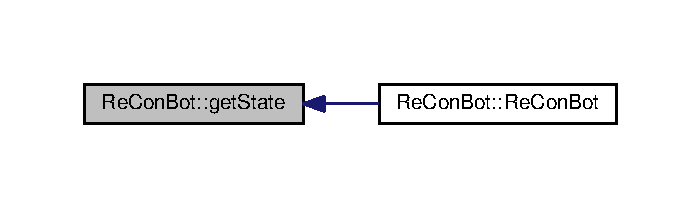
\includegraphics[width=336pt]{d9/d0b/class_re_con_bot_a3d9656755c06ded1f3b88ce05565f758_icgraph}
\end{center}
\end{figure}
\mbox{\Hypertarget{class_re_con_bot_lx_a0e25f573057755c6729ea572362652e6}\label{class_re_con_bot_lx_a0e25f573057755c6729ea572362652e6}} 
\index{Re\+Con\+Bot\+Lx@{Re\+Con\+Bot\+Lx}!motors\+State@{motors\+State}}
\index{motors\+State@{motors\+State}!Re\+Con\+Bot\+Lx@{Re\+Con\+Bot\+Lx}}
\subsubsection{\texorpdfstring{motors\+State()}{motorsState()}}
{\footnotesize\ttfamily void Re\+Con\+Bot\+Lx\+::motors\+State (\begin{DoxyParamCaption}\item[{int}]{arg\mbox{[}$\,$\mbox{]},  }\item[{int}]{length }\end{DoxyParamCaption})}



Definition at line 136 of file Re\+Con\+Bot.\+h.



References motors\+Active, and n\+Motors.



Referenced by main().


\begin{DoxyCode}
136                                                   \{
137   \textcolor{comment}{// First, the joint names, which apply to all waypoints}
138   \hyperlink{_re_con_bot_8h_a754c7486afa85fff30b8e7c0ce40c264}{motorsActive} = arg;
139   \hyperlink{_re_con_bot_8h_af9fc8046227b67fb8c85827f5ebc4838}{nMotors} = length;
140 \}
\end{DoxyCode}
Here is the caller graph for this function\+:
\nopagebreak
\begin{figure}[H]
\begin{center}
\leavevmode
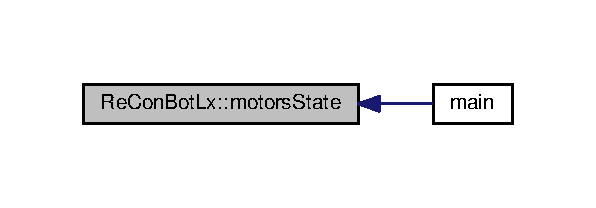
\includegraphics[width=286pt]{d2/d07/class_re_con_bot_lx_a0e25f573057755c6729ea572362652e6_icgraph}
\end{center}
\end{figure}
\mbox{\Hypertarget{class_re_con_bot_lx_a5d60b16962e5ce8e452f7c53543c54ce}\label{class_re_con_bot_lx_a5d60b16962e5ce8e452f7c53543c54ce}} 
\index{Re\+Con\+Bot\+Lx@{Re\+Con\+Bot\+Lx}!reconbot\+Callback@{reconbot\+Callback}}
\index{reconbot\+Callback@{reconbot\+Callback}!Re\+Con\+Bot\+Lx@{Re\+Con\+Bot\+Lx}}
\subsubsection{\texorpdfstring{reconbot\+Callback()}{reconbotCallback()}}
{\footnotesize\ttfamily void Re\+Con\+Bot\+Lx\+::reconbot\+Callback (\begin{DoxyParamCaption}\item[{const control\+\_\+msgs\+::\+Follow\+Joint\+Trajectory\+Goal}]{goal }\end{DoxyParamCaption})}



Definition at line 142 of file Re\+Con\+Bot.\+h.



References Re\+Con\+Bot\+::start\+Trajectory().



Referenced by main().


\begin{DoxyCode}
142                                                                                  \{
143       \hyperlink{class_re_con_bot_ade3eb1a4752d45659321209f5730cef3}{ReConBot::startTrajectory}(\hyperlink{class_re_con_bot_a9bd1c7ddf2376e2e68ea5d8bd8c3f505}{goal});
144   \}
\end{DoxyCode}
Here is the call graph for this function\+:
\nopagebreak
\begin{figure}[H]
\begin{center}
\leavevmode
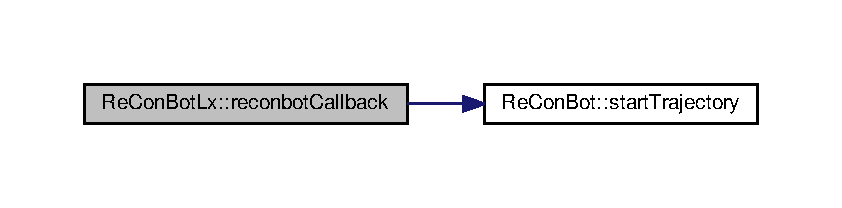
\includegraphics[width=350pt]{d2/d07/class_re_con_bot_lx_a5d60b16962e5ce8e452f7c53543c54ce_cgraph}
\end{center}
\end{figure}
Here is the caller graph for this function\+:
\nopagebreak
\begin{figure}[H]
\begin{center}
\leavevmode
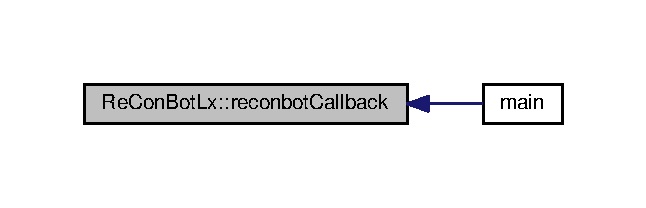
\includegraphics[width=310pt]{d2/d07/class_re_con_bot_lx_a5d60b16962e5ce8e452f7c53543c54ce_icgraph}
\end{center}
\end{figure}
\mbox{\Hypertarget{class_re_con_bot_ac264f3082203c3b2ef13b6f353476ca7}\label{class_re_con_bot_ac264f3082203c3b2ef13b6f353476ca7}} 
\index{Re\+Con\+Bot\+Lx@{Re\+Con\+Bot\+Lx}!run@{run}}
\index{run@{run}!Re\+Con\+Bot\+Lx@{Re\+Con\+Bot\+Lx}}
\subsubsection{\texorpdfstring{run()}{run()}}
{\footnotesize\ttfamily bool Re\+Con\+Bot\+::run (\begin{DoxyParamCaption}{ }\end{DoxyParamCaption})\hspace{0.3cm}{\ttfamily [inherited]}}

$<$Two spinner are instantiated for managing 2 threats 

Definition at line 118 of file Re\+Con\+Bot.\+h.



Referenced by Re\+Con\+Bot\+::\+Re\+Con\+Bot().


\begin{DoxyCode}
118                   \{
119     ros::AsyncSpinner spinner(2);
120     spinner.start();
121     ros::waitForShutdown();
122 \}
\end{DoxyCode}
Here is the caller graph for this function\+:
\nopagebreak
\begin{figure}[H]
\begin{center}
\leavevmode
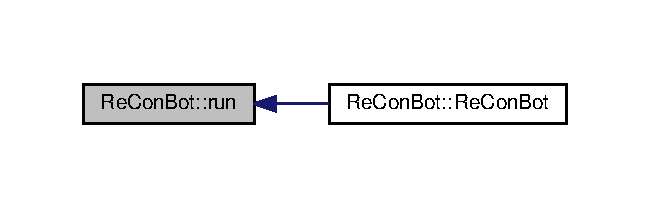
\includegraphics[width=312pt]{d9/d0b/class_re_con_bot_ac264f3082203c3b2ef13b6f353476ca7_icgraph}
\end{center}
\end{figure}
\mbox{\Hypertarget{class_re_con_bot_ade3eb1a4752d45659321209f5730cef3}\label{class_re_con_bot_ade3eb1a4752d45659321209f5730cef3}} 
\index{Re\+Con\+Bot\+Lx@{Re\+Con\+Bot\+Lx}!start\+Trajectory@{start\+Trajectory}}
\index{start\+Trajectory@{start\+Trajectory}!Re\+Con\+Bot\+Lx@{Re\+Con\+Bot\+Lx}}
\subsubsection{\texorpdfstring{start\+Trajectory()}{startTrajectory()}}
{\footnotesize\ttfamily void Re\+Con\+Bot\+::start\+Trajectory (\begin{DoxyParamCaption}\item[{control\+\_\+msgs\+::\+Follow\+Joint\+Trajectory\+Goal}]{goal }\end{DoxyParamCaption})\hspace{0.3cm}{\ttfamily [inherited]}}

Sends the command to start a given trajectory 

Definition at line 127 of file Re\+Con\+Bot.\+h.



References Re\+Con\+Bot\+::traj\+\_\+client\+\_\+.



Referenced by Re\+Con\+Bot\+::\+Re\+Con\+Bot(), and reconbot\+Callback().


\begin{DoxyCode}
127                                                                         \{
128   ROS\_INFO(\textcolor{stringliteral}{"=========== Welcome to IGM - ReConBot Move Group Interface =============="});
129   ROS\_INFO(\textcolor{stringliteral}{"=========== Group of Robotic and Mechatronic               =============="});
130 
131     \textcolor{comment}{// When to start the trajectory: 1s from now}
132     \hyperlink{class_re_con_bot_a9bd1c7ddf2376e2e68ea5d8bd8c3f505}{goal}.trajectory.header.stamp = ros::Time::now() + ros::Duration(1.0);
133     \hyperlink{class_re_con_bot_a14a35ad6ca284af7db7228d7872720d1}{traj\_client\_}->sendGoal(\hyperlink{class_re_con_bot_a9bd1c7ddf2376e2e68ea5d8bd8c3f505}{goal});
134   \}
\end{DoxyCode}
Here is the caller graph for this function\+:
\nopagebreak
\begin{figure}[H]
\begin{center}
\leavevmode
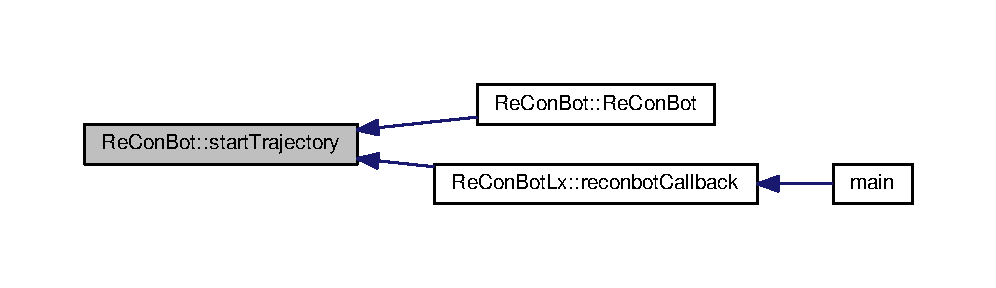
\includegraphics[width=350pt]{d9/d0b/class_re_con_bot_ade3eb1a4752d45659321209f5730cef3_icgraph}
\end{center}
\end{figure}
\mbox{\Hypertarget{class_re_con_bot_ab859fa96532995d3c1545aaa9db1802e}\label{class_re_con_bot_ab859fa96532995d3c1545aaa9db1802e}} 
\index{Re\+Con\+Bot\+Lx@{Re\+Con\+Bot\+Lx}!traj\+Client@{traj\+Client}}
\index{traj\+Client@{traj\+Client}!Re\+Con\+Bot\+Lx@{Re\+Con\+Bot\+Lx}}
\subsubsection{\texorpdfstring{traj\+Client()}{trajClient()}}
{\footnotesize\ttfamily void Re\+Con\+Bot\+::traj\+Client (\begin{DoxyParamCaption}{ }\end{DoxyParamCaption})\hspace{0.3cm}{\ttfamily [inherited]}}

tell the action client that we want to spin a thread by default

Definition at line 106 of file Re\+Con\+Bot.\+h.



References Re\+Con\+Bot\+::name\+Space, and Re\+Con\+Bot\+::traj\+\_\+client\+\_\+.



Referenced by main(), and Re\+Con\+Bot\+::\+Re\+Con\+Bot().


\begin{DoxyCode}
106                          \{
110   \hyperlink{class_re_con_bot_a14a35ad6ca284af7db7228d7872720d1}{traj\_client\_} = \textcolor{keyword}{new} \hyperlink{_re_con_bot_8h_a6fb8875093261cdc69e54d3ac7d5c301}{TrajClient}(\hyperlink{class_re_con_bot_a40ca07cd606988b78664c4a52fd8dc59}{nameSpace} + \textcolor{stringliteral}{"/follow\_joint\_trajectory"}, \textcolor{keyword}{true}
      );
111 
112   \textcolor{comment}{// wait for action server to come up}
113   \textcolor{keywordflow}{while}(!\hyperlink{class_re_con_bot_a14a35ad6ca284af7db7228d7872720d1}{traj\_client\_}->waitForServer(ros::Duration(5.0)))\{
114   ROS\_INFO(\textcolor{stringliteral}{"Waiting for the joint\_trajectory\_action server"});
115   \}
116 \}
\end{DoxyCode}
Here is the caller graph for this function\+:
\nopagebreak
\begin{figure}[H]
\begin{center}
\leavevmode
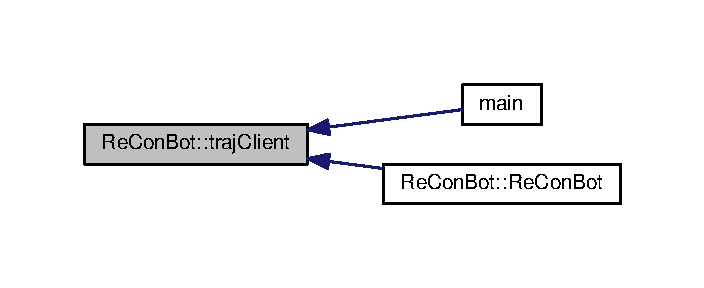
\includegraphics[width=338pt]{d9/d0b/class_re_con_bot_ab859fa96532995d3c1545aaa9db1802e_icgraph}
\end{center}
\end{figure}


\subsection{Member Data Documentation}
\mbox{\Hypertarget{class_re_con_bot_a9bd1c7ddf2376e2e68ea5d8bd8c3f505}\label{class_re_con_bot_a9bd1c7ddf2376e2e68ea5d8bd8c3f505}} 
\index{Re\+Con\+Bot\+Lx@{Re\+Con\+Bot\+Lx}!goal@{goal}}
\index{goal@{goal}!Re\+Con\+Bot\+Lx@{Re\+Con\+Bot\+Lx}}
\subsubsection{\texorpdfstring{goal}{goal}}
{\footnotesize\ttfamily control\+\_\+msgs\+::\+Follow\+Joint\+Trajectory\+Goal Re\+Con\+Bot\+::goal\hspace{0.3cm}{\ttfamily [protected]}, {\ttfamily [inherited]}}



Definition at line 60 of file Re\+Con\+Bot.\+h.



Referenced by Re\+Con\+Bot\+Pub\+::build\+Trajectory(), Re\+Con\+Bot\+Lx(), and Re\+Con\+Bot\+Pub\+::\+Re\+Con\+Bot\+Pub().

\mbox{\Hypertarget{class_re_con_bot_a40ca07cd606988b78664c4a52fd8dc59}\label{class_re_con_bot_a40ca07cd606988b78664c4a52fd8dc59}} 
\index{Re\+Con\+Bot\+Lx@{Re\+Con\+Bot\+Lx}!name\+Space@{name\+Space}}
\index{name\+Space@{name\+Space}!Re\+Con\+Bot\+Lx@{Re\+Con\+Bot\+Lx}}
\subsubsection{\texorpdfstring{name\+Space}{nameSpace}}
{\footnotesize\ttfamily std\+::string Re\+Con\+Bot\+::name\+Space\hspace{0.3cm}{\ttfamily [inherited]}}



Definition at line 68 of file Re\+Con\+Bot.\+h.



Referenced by main(), and Re\+Con\+Bot\+::traj\+Client().

\mbox{\Hypertarget{class_re_con_bot_a37edfe9c2dbbf37894c9bf850806fdd3}\label{class_re_con_bot_a37edfe9c2dbbf37894c9bf850806fdd3}} 
\index{Re\+Con\+Bot\+Lx@{Re\+Con\+Bot\+Lx}!nh\+Pub@{nh\+Pub}}
\index{nh\+Pub@{nh\+Pub}!Re\+Con\+Bot\+Lx@{Re\+Con\+Bot\+Lx}}
\subsubsection{\texorpdfstring{nh\+Pub}{nhPub}}
{\footnotesize\ttfamily ros\+::\+Node\+Handle Re\+Con\+Bot\+::nh\+Pub\hspace{0.3cm}{\ttfamily [protected]}, {\ttfamily [inherited]}}



Definition at line 61 of file Re\+Con\+Bot.\+h.



Referenced by Re\+Con\+Bot\+Pub\+::trajectory\+Publisher\+Start().

\mbox{\Hypertarget{class_re_con_bot_a549b7542d286b690f38b7ece8b83850b}\label{class_re_con_bot_a549b7542d286b690f38b7ece8b83850b}} 
\index{Re\+Con\+Bot\+Lx@{Re\+Con\+Bot\+Lx}!nh\+Pub\+\_\+pub@{nh\+Pub\+\_\+pub}}
\index{nh\+Pub\+\_\+pub@{nh\+Pub\+\_\+pub}!Re\+Con\+Bot\+Lx@{Re\+Con\+Bot\+Lx}}
\subsubsection{\texorpdfstring{nh\+Pub\+\_\+pub}{nhPub\_pub}}
{\footnotesize\ttfamily ros\+::\+Publisher Re\+Con\+Bot\+::nh\+Pub\+\_\+pub\hspace{0.3cm}{\ttfamily [protected]}, {\ttfamily [inherited]}}



Definition at line 62 of file Re\+Con\+Bot.\+h.



Referenced by Re\+Con\+Bot\+Pub\+::publisher(), and Re\+Con\+Bot\+Pub\+::trajectory\+Publisher\+Start().

\mbox{\Hypertarget{class_re_con_bot_a65cf4bed9bbabd92e1265d05507e0945}\label{class_re_con_bot_a65cf4bed9bbabd92e1265d05507e0945}} 
\index{Re\+Con\+Bot\+Lx@{Re\+Con\+Bot\+Lx}!source\+File@{source\+File}}
\index{source\+File@{source\+File}!Re\+Con\+Bot\+Lx@{Re\+Con\+Bot\+Lx}}
\subsubsection{\texorpdfstring{source\+File}{sourceFile}}
{\footnotesize\ttfamily std\+::string Re\+Con\+Bot\+::source\+File\hspace{0.3cm}{\ttfamily [inherited]}}

File directory with pose data 

Definition at line 67 of file Re\+Con\+Bot.\+h.



Referenced by Re\+Con\+Bot\+Pub\+::build\+Trajectory(), main(), and Re\+Con\+Bot\+Pub\+::\+Re\+Con\+Bot\+Pub().

\mbox{\Hypertarget{class_re_con_bot_a1d91d2ea8c0f16340440357906fb9ebf}\label{class_re_con_bot_a1d91d2ea8c0f16340440357906fb9ebf}} 
\index{Re\+Con\+Bot\+Lx@{Re\+Con\+Bot\+Lx}!topic\+Name@{topic\+Name}}
\index{topic\+Name@{topic\+Name}!Re\+Con\+Bot\+Lx@{Re\+Con\+Bot\+Lx}}
\subsubsection{\texorpdfstring{topic\+Name}{topicName}}
{\footnotesize\ttfamily std\+::string Re\+Con\+Bot\+::topic\+Name\hspace{0.3cm}{\ttfamily [inherited]}}

Name given to the topic where is publishing. 

Definition at line 69 of file Re\+Con\+Bot.\+h.



Referenced by main(), Re\+Con\+Bot\+Pub\+::\+Re\+Con\+Bot\+Pub(), and Re\+Con\+Bot\+Pub\+::trajectory\+Publisher\+Start().

\mbox{\Hypertarget{class_re_con_bot_aba20d307ac1b2e6b22f96da83a0d937d}\label{class_re_con_bot_aba20d307ac1b2e6b22f96da83a0d937d}} 
\index{Re\+Con\+Bot\+Lx@{Re\+Con\+Bot\+Lx}!topic\+Query@{topic\+Query}}
\index{topic\+Query@{topic\+Query}!Re\+Con\+Bot\+Lx@{Re\+Con\+Bot\+Lx}}
\subsubsection{\texorpdfstring{topic\+Query}{topicQuery}}
{\footnotesize\ttfamily int Re\+Con\+Bot\+::topic\+Query\hspace{0.3cm}{\ttfamily [protected]}, {\ttfamily [inherited]}}



Definition at line 63 of file Re\+Con\+Bot.\+h.



Referenced by Re\+Con\+Bot\+Pub\+::\+Re\+Con\+Bot\+Pub(), and Re\+Con\+Bot\+Pub\+::trajectory\+Publisher\+Start().

\mbox{\Hypertarget{class_re_con_bot_a14a35ad6ca284af7db7228d7872720d1}\label{class_re_con_bot_a14a35ad6ca284af7db7228d7872720d1}} 
\index{Re\+Con\+Bot\+Lx@{Re\+Con\+Bot\+Lx}!traj\+\_\+client\+\_\+@{traj\+\_\+client\+\_\+}}
\index{traj\+\_\+client\+\_\+@{traj\+\_\+client\+\_\+}!Re\+Con\+Bot\+Lx@{Re\+Con\+Bot\+Lx}}
\subsubsection{\texorpdfstring{traj\+\_\+client\+\_\+}{traj\_client\_}}
{\footnotesize\ttfamily \hyperlink{basic__arm_8cpp_a6fb8875093261cdc69e54d3ac7d5c301}{Traj\+Client}$\ast$ Re\+Con\+Bot\+::traj\+\_\+client\+\_\+\hspace{0.3cm}{\ttfamily [protected]}, {\ttfamily [inherited]}}



Definition at line 59 of file Re\+Con\+Bot.\+h.



Referenced by Re\+Con\+Bot\+::get\+State(), Re\+Con\+Bot\+::start\+Trajectory(), and Re\+Con\+Bot\+::traj\+Client().

\mbox{\Hypertarget{class_re_con_bot_a7c59e136741800bf0734f659119aa5ee}\label{class_re_con_bot_a7c59e136741800bf0734f659119aa5ee}} 
\index{Re\+Con\+Bot\+Lx@{Re\+Con\+Bot\+Lx}!trajectory\+Points@{trajectory\+Points}}
\index{trajectory\+Points@{trajectory\+Points}!Re\+Con\+Bot\+Lx@{Re\+Con\+Bot\+Lx}}
\subsubsection{\texorpdfstring{trajectory\+Points}{trajectoryPoints}}
{\footnotesize\ttfamily std\+::vector$<$double$>$ Re\+Con\+Bot\+::trajectory\+Points\hspace{0.3cm}{\ttfamily [protected]}, {\ttfamily [inherited]}}



Definition at line 64 of file Re\+Con\+Bot.\+h.



Referenced by Re\+Con\+Bot\+Pub\+::build\+Trajectory().



The documentation for this class was generated from the following file\+:\begin{DoxyCompactItemize}
\item 
\hyperlink{_re_con_bot_8h}{Re\+Con\+Bot.\+h}\end{DoxyCompactItemize}

\hypertarget{class_re_con_bot_pub}{}\section{Re\+Con\+Bot\+Pub Class Reference}
\label{class_re_con_bot_pub}\index{Re\+Con\+Bot\+Pub@{Re\+Con\+Bot\+Pub}}


{\ttfamily \#include $<$Re\+Con\+Bot.\+h$>$}



Inheritance diagram for Re\+Con\+Bot\+Pub\+:\nopagebreak
\begin{figure}[H]
\begin{center}
\leavevmode
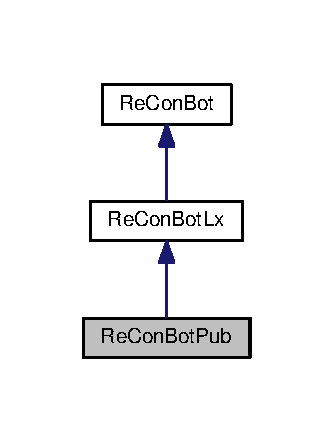
\includegraphics[width=160pt]{d3/d0f/class_re_con_bot_pub__inherit__graph}
\end{center}
\end{figure}


Collaboration diagram for Re\+Con\+Bot\+Pub\+:\nopagebreak
\begin{figure}[H]
\begin{center}
\leavevmode
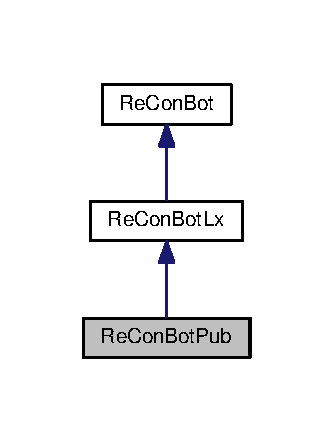
\includegraphics[width=160pt]{dc/d8a/class_re_con_bot_pub__coll__graph}
\end{center}
\end{figure}
\subsection*{Public Member Functions}
\begin{DoxyCompactItemize}
\item 
\hyperlink{class_re_con_bot_pub_a3e761c430b2934ad96e499dcd8bd67e2}{Re\+Con\+Bot\+Pub} ()
\item 
control\+\_\+msgs\+::\+Follow\+Joint\+Trajectory\+Goal \hyperlink{class_re_con_bot_pub_af99f5189cd8e834d7b59f1b106b99345}{build\+Trajectory} ()
\item 
void \hyperlink{class_re_con_bot_pub_a2019b0d8d30f2419026c90dd30de500f}{trajectory\+Publisher\+Start} (ros\+::\+Node\+Handle \&nh, int \hyperlink{class_re_con_bot_aba20d307ac1b2e6b22f96da83a0d937d}{topic\+Query})
\item 
void \hyperlink{class_re_con_bot_pub_ac763949cb5256de695e02c5f81084ead}{publisher} (control\+\_\+msgs\+::\+Follow\+Joint\+Trajectory\+Goal \hyperlink{class_re_con_bot_a9bd1c7ddf2376e2e68ea5d8bd8c3f505}{goal})
\item 
void \hyperlink{class_re_con_bot_lx_a0e25f573057755c6729ea572362652e6}{motors\+State} (int arg\mbox{[}$\,$\mbox{]}, int length)
\item 
void \hyperlink{class_re_con_bot_lx_a5d60b16962e5ce8e452f7c53543c54ce}{reconbot\+Callback} (const control\+\_\+msgs\+::\+Follow\+Joint\+Trajectory\+Goal \hyperlink{class_re_con_bot_a9bd1c7ddf2376e2e68ea5d8bd8c3f505}{goal})
\item 
void \hyperlink{class_re_con_bot_ab859fa96532995d3c1545aaa9db1802e}{traj\+Client} ()
\item 
void \hyperlink{class_re_con_bot_ade3eb1a4752d45659321209f5730cef3}{start\+Trajectory} (control\+\_\+msgs\+::\+Follow\+Joint\+Trajectory\+Goal \hyperlink{class_re_con_bot_a9bd1c7ddf2376e2e68ea5d8bd8c3f505}{goal})
\item 
control\+\_\+msgs\+::\+Follow\+Joint\+Trajectory\+Goal \hyperlink{class_re_con_bot_a950f2769ca61ff7b663d86ed2cf19c14}{arm\+Trajectory} ()
\item 
bool \hyperlink{class_re_con_bot_ac264f3082203c3b2ef13b6f353476ca7}{run} ()
\item 
actionlib\+::\+Simple\+Client\+Goal\+State \hyperlink{class_re_con_bot_a3d9656755c06ded1f3b88ce05565f758}{get\+State} ()
\begin{DoxyCompactList}\small\item\em Returns the current state of the action. \end{DoxyCompactList}\end{DoxyCompactItemize}
\subsection*{Public Attributes}
\begin{DoxyCompactItemize}
\item 
std\+::string \hyperlink{class_re_con_bot_a65cf4bed9bbabd92e1265d05507e0945}{source\+File}
\item 
std\+::string \hyperlink{class_re_con_bot_a40ca07cd606988b78664c4a52fd8dc59}{name\+Space}
\item 
std\+::string \hyperlink{class_re_con_bot_a1d91d2ea8c0f16340440357906fb9ebf}{topic\+Name}
\end{DoxyCompactItemize}
\subsection*{Protected Attributes}
\begin{DoxyCompactItemize}
\item 
int \hyperlink{class_re_con_bot_pub_a2b0249f374eb7a6ab7741a85d8ebd9d5}{cont}
\item 
int \hyperlink{class_re_con_bot_pub_ac2d5ba45905a24cfbdd78bce2dfe2a4f}{var}
\item 
int \hyperlink{class_re_con_bot_pub_a1d9d82f366eeb794ffa28630de286710}{j}
\item 
float \hyperlink{class_re_con_bot_pub_a51311eed78ce3a444b35924c64ad3f4c}{pos}
\item 
\hyperlink{basic__arm_8cpp_a6fb8875093261cdc69e54d3ac7d5c301}{Traj\+Client} $\ast$ \hyperlink{class_re_con_bot_a14a35ad6ca284af7db7228d7872720d1}{traj\+\_\+client\+\_\+}
\item 
control\+\_\+msgs\+::\+Follow\+Joint\+Trajectory\+Goal \hyperlink{class_re_con_bot_a9bd1c7ddf2376e2e68ea5d8bd8c3f505}{goal}
\item 
ros\+::\+Node\+Handle \hyperlink{class_re_con_bot_a37edfe9c2dbbf37894c9bf850806fdd3}{nh\+Pub}
\item 
ros\+::\+Publisher \hyperlink{class_re_con_bot_a549b7542d286b690f38b7ece8b83850b}{nh\+Pub\+\_\+pub}
\item 
int \hyperlink{class_re_con_bot_aba20d307ac1b2e6b22f96da83a0d937d}{topic\+Query}
\item 
std\+::vector$<$ double $>$ \hyperlink{class_re_con_bot_a7c59e136741800bf0734f659119aa5ee}{trajectory\+Points}
\end{DoxyCompactItemize}


\subsection{Detailed Description}


Definition at line 88 of file Re\+Con\+Bot.\+h.



\subsection{Constructor \& Destructor Documentation}
\mbox{\Hypertarget{class_re_con_bot_pub_a3e761c430b2934ad96e499dcd8bd67e2}\label{class_re_con_bot_pub_a3e761c430b2934ad96e499dcd8bd67e2}} 
\index{Re\+Con\+Bot\+Pub@{Re\+Con\+Bot\+Pub}!Re\+Con\+Bot\+Pub@{Re\+Con\+Bot\+Pub}}
\index{Re\+Con\+Bot\+Pub@{Re\+Con\+Bot\+Pub}!Re\+Con\+Bot\+Pub@{Re\+Con\+Bot\+Pub}}
\subsubsection{\texorpdfstring{Re\+Con\+Bot\+Pub()}{ReConBotPub()}}
{\footnotesize\ttfamily Re\+Con\+Bot\+Pub\+::\+Re\+Con\+Bot\+Pub (\begin{DoxyParamCaption}{ }\end{DoxyParamCaption})\hspace{0.3cm}{\ttfamily [inline]}}



Definition at line 96 of file Re\+Con\+Bot.\+h.



References Re\+Con\+Bot\+::goal, Re\+Con\+Bot\+::source\+File, Re\+Con\+Bot\+::topic\+Name, and Re\+Con\+Bot\+::topic\+Query.


\begin{DoxyCode}
96                \{
97     \hyperlink{class_re_con_bot_a65cf4bed9bbabd92e1265d05507e0945}{sourceFile} = \textcolor{stringliteral}{"/home/jdelacruz/catkin\_ws/src/reconbot/trajectory/trajectory1.txt"};
98     \hyperlink{class_re_con_bot_a1d91d2ea8c0f16340440357906fb9ebf}{topicName} = \textcolor{stringliteral}{"/reconbot\_trajectory"};
99   \}
\end{DoxyCode}


\subsection{Member Function Documentation}
\mbox{\Hypertarget{class_re_con_bot_a950f2769ca61ff7b663d86ed2cf19c14}\label{class_re_con_bot_a950f2769ca61ff7b663d86ed2cf19c14}} 
\index{Re\+Con\+Bot\+Pub@{Re\+Con\+Bot\+Pub}!arm\+Trajectory@{arm\+Trajectory}}
\index{arm\+Trajectory@{arm\+Trajectory}!Re\+Con\+Bot\+Pub@{Re\+Con\+Bot\+Pub}}
\subsubsection{\texorpdfstring{arm\+Trajectory()}{armTrajectory()}}
{\footnotesize\ttfamily control\+\_\+msgs\+::\+Follow\+Joint\+Trajectory\+Goal Re\+Con\+Bot\+::arm\+Trajectory (\begin{DoxyParamCaption}{ }\end{DoxyParamCaption})\hspace{0.3cm}{\ttfamily [inherited]}}



Referenced by Re\+Con\+Bot\+::\+Re\+Con\+Bot().

Here is the caller graph for this function\+:\nopagebreak
\begin{figure}[H]
\begin{center}
\leavevmode
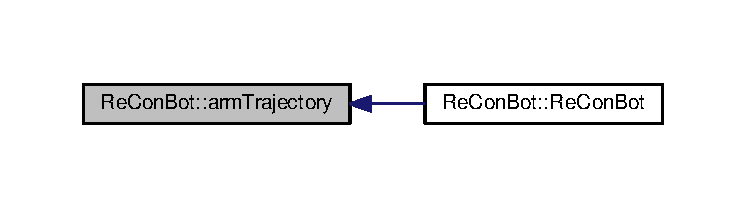
\includegraphics[width=350pt]{d9/d0b/class_re_con_bot_a950f2769ca61ff7b663d86ed2cf19c14_icgraph}
\end{center}
\end{figure}
\mbox{\Hypertarget{class_re_con_bot_pub_af99f5189cd8e834d7b59f1b106b99345}\label{class_re_con_bot_pub_af99f5189cd8e834d7b59f1b106b99345}} 
\index{Re\+Con\+Bot\+Pub@{Re\+Con\+Bot\+Pub}!build\+Trajectory@{build\+Trajectory}}
\index{build\+Trajectory@{build\+Trajectory}!Re\+Con\+Bot\+Pub@{Re\+Con\+Bot\+Pub}}
\subsubsection{\texorpdfstring{build\+Trajectory()}{buildTrajectory()}}
{\footnotesize\ttfamily control\+\_\+msgs\+::\+Follow\+Joint\+Trajectory\+Goal Re\+Con\+Bot\+Pub\+::build\+Trajectory (\begin{DoxyParamCaption}{ }\end{DoxyParamCaption})}



Definition at line 175 of file Re\+Con\+Bot.\+h.



References Re\+Con\+Bot\+::goal, motors\+Active, n\+Motors, Re\+Con\+Bot\+::source\+File, and Re\+Con\+Bot\+::trajectory\+Points.



Referenced by main().


\begin{DoxyCode}
175                                                                   \{
176   ROS\_INFO(\textcolor{stringliteral}{"Start building the Trajectory Vector..."});
177   \textcolor{keywordflow}{for} (\textcolor{keywordtype}{size\_t} i = 0; i < \hyperlink{_re_con_bot_8h_af9fc8046227b67fb8c85827f5ebc4838}{nMotors}; i++) \{
178     std::stringstream ss;
179     ss << \hyperlink{_re_con_bot_8h_a754c7486afa85fff30b8e7c0ce40c264}{motorsActive}[i];
180     \hyperlink{class_re_con_bot_a9bd1c7ddf2376e2e68ea5d8bd8c3f505}{goal}.trajectory.joint\_names.push\_back(\textcolor{stringliteral}{"joint\_"}+ ss.str());
181   \}
182   \textcolor{comment}{//goal.trajectory.joint\_names.push\_back("joint\_1");}
183   \textcolor{comment}{//goal.trajectory.joint\_names.push\_back("joint\_2");}
184   \textcolor{comment}{//goal.trajectory.joint\_names.push\_back("joint\_3");}
185 
186   std::fstream pathfile(\hyperlink{class_re_con_bot_a65cf4bed9bbabd92e1265d05507e0945}{sourceFile}.c\_str(), std::ios\_base::in);
187   \textcolor{keywordtype}{int} number\_of\_lines = 0;
188   std::string line;
189   std::ifstream myfile(\hyperlink{class_re_con_bot_a65cf4bed9bbabd92e1265d05507e0945}{sourceFile}.c\_str());
190 
191   \textcolor{keywordflow}{while} (std::getline(myfile, line))\{
192       ++number\_of\_lines;
193     \}
194   \hyperlink{class_re_con_bot_a9bd1c7ddf2376e2e68ea5d8bd8c3f505}{goal}.trajectory.points.resize(number\_of\_lines);
195   \hyperlink{class_re_con_bot_pub_a2b0249f374eb7a6ab7741a85d8ebd9d5}{cont} =0;
196   \hyperlink{class_re_con_bot_pub_ac2d5ba45905a24cfbdd78bce2dfe2a4f}{var} =0;
197   \textcolor{keywordflow}{while} (pathfile >> \hyperlink{class_re_con_bot_pub_a51311eed78ce3a444b35924c64ad3f4c}{pos} && ros::ok()) \{
198     \hyperlink{class_re_con_bot_a7c59e136741800bf0734f659119aa5ee}{trajectoryPoints}.resize(number\_of\_lines*(nMotors*3+1));
199     \hyperlink{class_re_con_bot_a7c59e136741800bf0734f659119aa5ee}{trajectoryPoints}[\hyperlink{class_re_con_bot_pub_ac2d5ba45905a24cfbdd78bce2dfe2a4f}{var}]=\hyperlink{class_re_con_bot_pub_a51311eed78ce3a444b35924c64ad3f4c}{pos};
200     ++\hyperlink{class_re_con_bot_pub_ac2d5ba45905a24cfbdd78bce2dfe2a4f}{var};
201     \textcolor{keywordflow}{if} (\hyperlink{class_re_con_bot_pub_ac2d5ba45905a24cfbdd78bce2dfe2a4f}{var} == nMotors*3 + 1) \{
202       \hyperlink{class_re_con_bot_pub_a1d9d82f366eeb794ffa28630de286710}{j} = 0;
203       \textcolor{keywordflow}{for} (\textcolor{keywordtype}{size\_t} i = 0; i < nMotors*3; i=i+3) \{
204         \hyperlink{class_re_con_bot_a9bd1c7ddf2376e2e68ea5d8bd8c3f505}{goal}.trajectory.points[\hyperlink{class_re_con_bot_pub_a2b0249f374eb7a6ab7741a85d8ebd9d5}{cont}].positions.resize(nMotors);
205         \hyperlink{class_re_con_bot_a9bd1c7ddf2376e2e68ea5d8bd8c3f505}{goal}.trajectory.points[\hyperlink{class_re_con_bot_pub_a2b0249f374eb7a6ab7741a85d8ebd9d5}{cont}].positions[\hyperlink{class_re_con_bot_pub_a1d9d82f366eeb794ffa28630de286710}{j}] = \hyperlink{class_re_con_bot_a7c59e136741800bf0734f659119aa5ee}{trajectoryPoints}[i];
206         ++\hyperlink{class_re_con_bot_pub_a1d9d82f366eeb794ffa28630de286710}{j};
207       \}
208       \hyperlink{class_re_con_bot_pub_a1d9d82f366eeb794ffa28630de286710}{j} = 0;
209       \textcolor{keywordflow}{for} (\textcolor{keywordtype}{size\_t} i = 1; i < nMotors*3; i=i+3) \{
210         \hyperlink{class_re_con_bot_a9bd1c7ddf2376e2e68ea5d8bd8c3f505}{goal}.trajectory.points[\hyperlink{class_re_con_bot_pub_a2b0249f374eb7a6ab7741a85d8ebd9d5}{cont}].velocities.resize(nMotors);
211         \hyperlink{class_re_con_bot_a9bd1c7ddf2376e2e68ea5d8bd8c3f505}{goal}.trajectory.points[\hyperlink{class_re_con_bot_pub_a2b0249f374eb7a6ab7741a85d8ebd9d5}{cont}].velocities[\hyperlink{class_re_con_bot_pub_a1d9d82f366eeb794ffa28630de286710}{j}] = \hyperlink{class_re_con_bot_a7c59e136741800bf0734f659119aa5ee}{trajectoryPoints}[i];
212         ++\hyperlink{class_re_con_bot_pub_a1d9d82f366eeb794ffa28630de286710}{j};\textcolor{comment}{/* condition */}
213       \}
214       \hyperlink{class_re_con_bot_pub_a1d9d82f366eeb794ffa28630de286710}{j} = 0;
215       \textcolor{keywordflow}{for} (\textcolor{keywordtype}{size\_t} i = 2; i < nMotors*3; i=i+3) \{
216         \hyperlink{class_re_con_bot_a9bd1c7ddf2376e2e68ea5d8bd8c3f505}{goal}.trajectory.points[\hyperlink{class_re_con_bot_pub_a2b0249f374eb7a6ab7741a85d8ebd9d5}{cont}].accelerations.resize(nMotors);
217         \hyperlink{class_re_con_bot_a9bd1c7ddf2376e2e68ea5d8bd8c3f505}{goal}.trajectory.points[\hyperlink{class_re_con_bot_pub_a2b0249f374eb7a6ab7741a85d8ebd9d5}{cont}].accelerations[\hyperlink{class_re_con_bot_pub_a1d9d82f366eeb794ffa28630de286710}{j}] = 
      \hyperlink{class_re_con_bot_a7c59e136741800bf0734f659119aa5ee}{trajectoryPoints}[i];
218         \textcolor{keywordflow}{if} (i == nMotors*3 - 1) \{
219           \hyperlink{class_re_con_bot_a9bd1c7ddf2376e2e68ea5d8bd8c3f505}{goal}.trajectory.points[\hyperlink{class_re_con_bot_pub_a2b0249f374eb7a6ab7741a85d8ebd9d5}{cont}].time\_from\_start = ros::Duration(
      \hyperlink{class_re_con_bot_a7c59e136741800bf0734f659119aa5ee}{trajectoryPoints}[i+1]);
220         \}
221         ++\hyperlink{class_re_con_bot_pub_a1d9d82f366eeb794ffa28630de286710}{j};
222       \}
223       \hyperlink{class_re_con_bot_pub_ac2d5ba45905a24cfbdd78bce2dfe2a4f}{var} = 0;
224       ++\hyperlink{class_re_con_bot_pub_a2b0249f374eb7a6ab7741a85d8ebd9d5}{cont};
225       ROS\_INFO(\textcolor{stringliteral}{"New trajectory point created..."});
226     \}
227   \}
228   ROS\_INFO(\textcolor{stringliteral}{"Trajectory vector was successfully built...."});
229   \textcolor{keywordflow}{return} \hyperlink{class_re_con_bot_a9bd1c7ddf2376e2e68ea5d8bd8c3f505}{goal};
230 \}
\end{DoxyCode}
Here is the caller graph for this function\+:\nopagebreak
\begin{figure}[H]
\begin{center}
\leavevmode
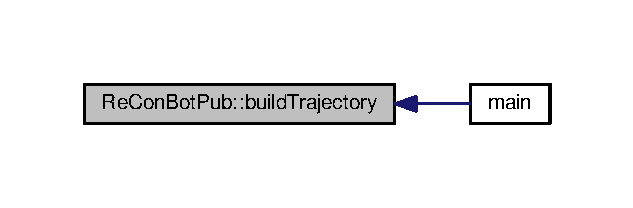
\includegraphics[width=304pt]{d6/d1b/class_re_con_bot_pub_af99f5189cd8e834d7b59f1b106b99345_icgraph}
\end{center}
\end{figure}
\mbox{\Hypertarget{class_re_con_bot_a3d9656755c06ded1f3b88ce05565f758}\label{class_re_con_bot_a3d9656755c06ded1f3b88ce05565f758}} 
\index{Re\+Con\+Bot\+Pub@{Re\+Con\+Bot\+Pub}!get\+State@{get\+State}}
\index{get\+State@{get\+State}!Re\+Con\+Bot\+Pub@{Re\+Con\+Bot\+Pub}}
\subsubsection{\texorpdfstring{get\+State()}{getState()}}
{\footnotesize\ttfamily actionlib\+::\+Simple\+Client\+Goal\+State Re\+Con\+Bot\+::get\+State (\begin{DoxyParamCaption}{ }\end{DoxyParamCaption})\hspace{0.3cm}{\ttfamily [inherited]}}



Returns the current state of the action. 



Definition at line 147 of file Re\+Con\+Bot.\+h.



References Re\+Con\+Bot\+::traj\+\_\+client\+\_\+.



Referenced by Re\+Con\+Bot\+::\+Re\+Con\+Bot().


\begin{DoxyCode}
147                                                  \{
148   \textcolor{keywordflow}{return} \hyperlink{class_re_con_bot_a14a35ad6ca284af7db7228d7872720d1}{traj\_client\_}->getState();
149 \}
\end{DoxyCode}
Here is the caller graph for this function\+:
\nopagebreak
\begin{figure}[H]
\begin{center}
\leavevmode
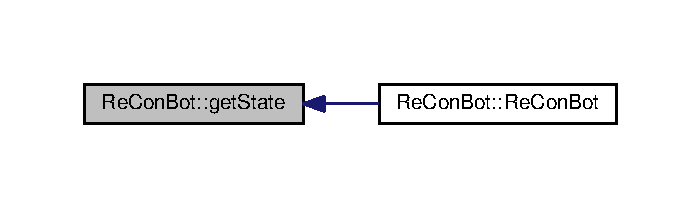
\includegraphics[width=336pt]{d9/d0b/class_re_con_bot_a3d9656755c06ded1f3b88ce05565f758_icgraph}
\end{center}
\end{figure}
\mbox{\Hypertarget{class_re_con_bot_lx_a0e25f573057755c6729ea572362652e6}\label{class_re_con_bot_lx_a0e25f573057755c6729ea572362652e6}} 
\index{Re\+Con\+Bot\+Pub@{Re\+Con\+Bot\+Pub}!motors\+State@{motors\+State}}
\index{motors\+State@{motors\+State}!Re\+Con\+Bot\+Pub@{Re\+Con\+Bot\+Pub}}
\subsubsection{\texorpdfstring{motors\+State()}{motorsState()}}
{\footnotesize\ttfamily void Re\+Con\+Bot\+Lx\+::motors\+State (\begin{DoxyParamCaption}\item[{int}]{arg\mbox{[}$\,$\mbox{]},  }\item[{int}]{length }\end{DoxyParamCaption})\hspace{0.3cm}{\ttfamily [inherited]}}



Definition at line 136 of file Re\+Con\+Bot.\+h.



References motors\+Active, and n\+Motors.



Referenced by main().


\begin{DoxyCode}
136                                                   \{
137   \textcolor{comment}{// First, the joint names, which apply to all waypoints}
138   \hyperlink{_re_con_bot_8h_a754c7486afa85fff30b8e7c0ce40c264}{motorsActive} = arg;
139   \hyperlink{_re_con_bot_8h_af9fc8046227b67fb8c85827f5ebc4838}{nMotors} = length;
140 \}
\end{DoxyCode}
Here is the caller graph for this function\+:
\nopagebreak
\begin{figure}[H]
\begin{center}
\leavevmode
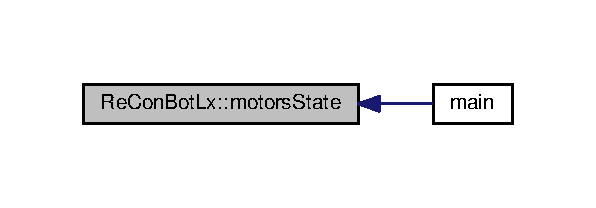
\includegraphics[width=286pt]{d2/d07/class_re_con_bot_lx_a0e25f573057755c6729ea572362652e6_icgraph}
\end{center}
\end{figure}
\mbox{\Hypertarget{class_re_con_bot_pub_ac763949cb5256de695e02c5f81084ead}\label{class_re_con_bot_pub_ac763949cb5256de695e02c5f81084ead}} 
\index{Re\+Con\+Bot\+Pub@{Re\+Con\+Bot\+Pub}!publisher@{publisher}}
\index{publisher@{publisher}!Re\+Con\+Bot\+Pub@{Re\+Con\+Bot\+Pub}}
\subsubsection{\texorpdfstring{publisher()}{publisher()}}
{\footnotesize\ttfamily void Re\+Con\+Bot\+Pub\+::publisher (\begin{DoxyParamCaption}\item[{control\+\_\+msgs\+::\+Follow\+Joint\+Trajectory\+Goal}]{goal }\end{DoxyParamCaption})}



Definition at line 156 of file Re\+Con\+Bot.\+h.



References Re\+Con\+Bot\+::nh\+Pub\+\_\+pub.



Referenced by main().


\begin{DoxyCode}
156                                                                      \{
157   \textcolor{keywordtype}{int} flag =0;
158   \textcolor{keywordflow}{while} (ros::ok()&&flag==0) \{
159     ROS\_INFO(\textcolor{stringliteral}{"Waiting for Subscribers..."});
160   \textcolor{comment}{//ros::Rate loop\_rate(0.1);}
161   \textcolor{comment}{//nhPub\_pub.publish(goal);}
162   \textcolor{comment}{//ros::spinOnce();}
163   \textcolor{comment}{//loop\_rate.sleep();}
164   \textcolor{comment}{//ros::spinOnce();}
165   \textcolor{comment}{//ROS\_INFO("Goal published");}
166 \textcolor{comment}{//\}}
167     \textcolor{keywordflow}{if} (\hyperlink{class_re_con_bot_a549b7542d286b690f38b7ece8b83850b}{nhPub\_pub}.getNumSubscribers()>= 1 && flag == 0) \{
168       \hyperlink{class_re_con_bot_a549b7542d286b690f38b7ece8b83850b}{nhPub\_pub}.publish(\hyperlink{class_re_con_bot_a9bd1c7ddf2376e2e68ea5d8bd8c3f505}{goal});
169       ros::spinOnce();
170       ROS\_INFO(\textcolor{stringliteral}{"Goal published!"});
171       flag = 1;
172     \}
173   \}
174 \}
\end{DoxyCode}
Here is the caller graph for this function\+:\nopagebreak
\begin{figure}[H]
\begin{center}
\leavevmode
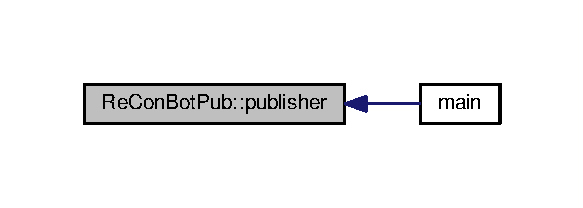
\includegraphics[width=280pt]{d6/d1b/class_re_con_bot_pub_ac763949cb5256de695e02c5f81084ead_icgraph}
\end{center}
\end{figure}
\mbox{\Hypertarget{class_re_con_bot_lx_a5d60b16962e5ce8e452f7c53543c54ce}\label{class_re_con_bot_lx_a5d60b16962e5ce8e452f7c53543c54ce}} 
\index{Re\+Con\+Bot\+Pub@{Re\+Con\+Bot\+Pub}!reconbot\+Callback@{reconbot\+Callback}}
\index{reconbot\+Callback@{reconbot\+Callback}!Re\+Con\+Bot\+Pub@{Re\+Con\+Bot\+Pub}}
\subsubsection{\texorpdfstring{reconbot\+Callback()}{reconbotCallback()}}
{\footnotesize\ttfamily void Re\+Con\+Bot\+Lx\+::reconbot\+Callback (\begin{DoxyParamCaption}\item[{const control\+\_\+msgs\+::\+Follow\+Joint\+Trajectory\+Goal}]{goal }\end{DoxyParamCaption})\hspace{0.3cm}{\ttfamily [inherited]}}



Definition at line 142 of file Re\+Con\+Bot.\+h.



References Re\+Con\+Bot\+::start\+Trajectory().



Referenced by main().


\begin{DoxyCode}
142                                                                                  \{
143       \hyperlink{class_re_con_bot_ade3eb1a4752d45659321209f5730cef3}{ReConBot::startTrajectory}(\hyperlink{class_re_con_bot_a9bd1c7ddf2376e2e68ea5d8bd8c3f505}{goal});
144   \}
\end{DoxyCode}
Here is the call graph for this function\+:
\nopagebreak
\begin{figure}[H]
\begin{center}
\leavevmode
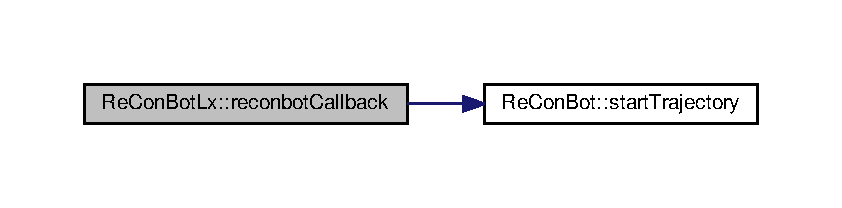
\includegraphics[width=350pt]{d2/d07/class_re_con_bot_lx_a5d60b16962e5ce8e452f7c53543c54ce_cgraph}
\end{center}
\end{figure}
Here is the caller graph for this function\+:
\nopagebreak
\begin{figure}[H]
\begin{center}
\leavevmode
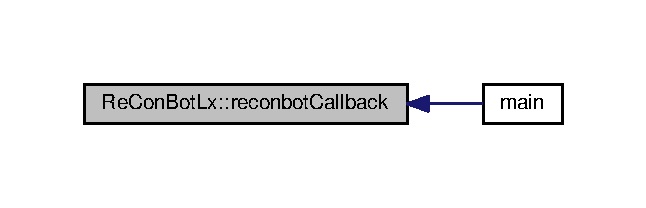
\includegraphics[width=310pt]{d2/d07/class_re_con_bot_lx_a5d60b16962e5ce8e452f7c53543c54ce_icgraph}
\end{center}
\end{figure}
\mbox{\Hypertarget{class_re_con_bot_ac264f3082203c3b2ef13b6f353476ca7}\label{class_re_con_bot_ac264f3082203c3b2ef13b6f353476ca7}} 
\index{Re\+Con\+Bot\+Pub@{Re\+Con\+Bot\+Pub}!run@{run}}
\index{run@{run}!Re\+Con\+Bot\+Pub@{Re\+Con\+Bot\+Pub}}
\subsubsection{\texorpdfstring{run()}{run()}}
{\footnotesize\ttfamily bool Re\+Con\+Bot\+::run (\begin{DoxyParamCaption}{ }\end{DoxyParamCaption})\hspace{0.3cm}{\ttfamily [inherited]}}

$<$Two spinner are instantiated for managing 2 threats 

Definition at line 118 of file Re\+Con\+Bot.\+h.



Referenced by Re\+Con\+Bot\+::\+Re\+Con\+Bot().


\begin{DoxyCode}
118                   \{
119     ros::AsyncSpinner spinner(2);
120     spinner.start();
121     ros::waitForShutdown();
122 \}
\end{DoxyCode}
Here is the caller graph for this function\+:
\nopagebreak
\begin{figure}[H]
\begin{center}
\leavevmode
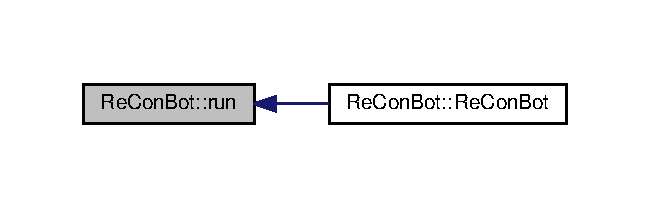
\includegraphics[width=312pt]{d9/d0b/class_re_con_bot_ac264f3082203c3b2ef13b6f353476ca7_icgraph}
\end{center}
\end{figure}
\mbox{\Hypertarget{class_re_con_bot_ade3eb1a4752d45659321209f5730cef3}\label{class_re_con_bot_ade3eb1a4752d45659321209f5730cef3}} 
\index{Re\+Con\+Bot\+Pub@{Re\+Con\+Bot\+Pub}!start\+Trajectory@{start\+Trajectory}}
\index{start\+Trajectory@{start\+Trajectory}!Re\+Con\+Bot\+Pub@{Re\+Con\+Bot\+Pub}}
\subsubsection{\texorpdfstring{start\+Trajectory()}{startTrajectory()}}
{\footnotesize\ttfamily void Re\+Con\+Bot\+::start\+Trajectory (\begin{DoxyParamCaption}\item[{control\+\_\+msgs\+::\+Follow\+Joint\+Trajectory\+Goal}]{goal }\end{DoxyParamCaption})\hspace{0.3cm}{\ttfamily [inherited]}}

Sends the command to start a given trajectory 

Definition at line 127 of file Re\+Con\+Bot.\+h.



References Re\+Con\+Bot\+::traj\+\_\+client\+\_\+.



Referenced by Re\+Con\+Bot\+::\+Re\+Con\+Bot(), and Re\+Con\+Bot\+Lx\+::reconbot\+Callback().


\begin{DoxyCode}
127                                                                         \{
128   ROS\_INFO(\textcolor{stringliteral}{"=========== Welcome to IGM - ReConBot Move Group Interface =============="});
129   ROS\_INFO(\textcolor{stringliteral}{"=========== Group of Robotic and Mechatronic               =============="});
130 
131     \textcolor{comment}{// When to start the trajectory: 1s from now}
132     \hyperlink{class_re_con_bot_a9bd1c7ddf2376e2e68ea5d8bd8c3f505}{goal}.trajectory.header.stamp = ros::Time::now() + ros::Duration(1.0);
133     \hyperlink{class_re_con_bot_a14a35ad6ca284af7db7228d7872720d1}{traj\_client\_}->sendGoal(\hyperlink{class_re_con_bot_a9bd1c7ddf2376e2e68ea5d8bd8c3f505}{goal});
134   \}
\end{DoxyCode}
Here is the caller graph for this function\+:
\nopagebreak
\begin{figure}[H]
\begin{center}
\leavevmode
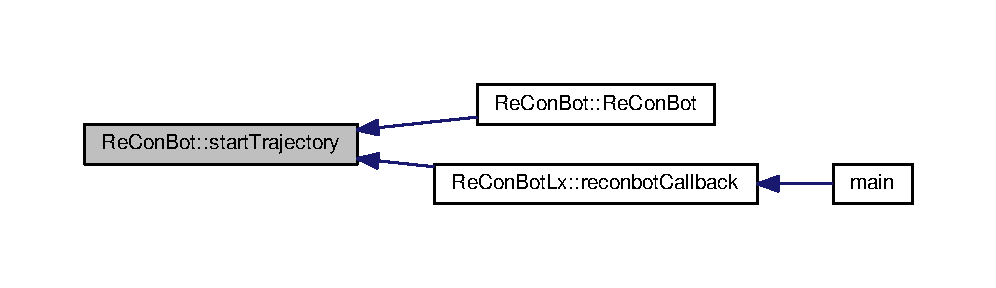
\includegraphics[width=350pt]{d9/d0b/class_re_con_bot_ade3eb1a4752d45659321209f5730cef3_icgraph}
\end{center}
\end{figure}
\mbox{\Hypertarget{class_re_con_bot_ab859fa96532995d3c1545aaa9db1802e}\label{class_re_con_bot_ab859fa96532995d3c1545aaa9db1802e}} 
\index{Re\+Con\+Bot\+Pub@{Re\+Con\+Bot\+Pub}!traj\+Client@{traj\+Client}}
\index{traj\+Client@{traj\+Client}!Re\+Con\+Bot\+Pub@{Re\+Con\+Bot\+Pub}}
\subsubsection{\texorpdfstring{traj\+Client()}{trajClient()}}
{\footnotesize\ttfamily void Re\+Con\+Bot\+::traj\+Client (\begin{DoxyParamCaption}{ }\end{DoxyParamCaption})\hspace{0.3cm}{\ttfamily [inherited]}}

tell the action client that we want to spin a thread by default

Definition at line 106 of file Re\+Con\+Bot.\+h.



References Re\+Con\+Bot\+::name\+Space, and Re\+Con\+Bot\+::traj\+\_\+client\+\_\+.



Referenced by main(), and Re\+Con\+Bot\+::\+Re\+Con\+Bot().


\begin{DoxyCode}
106                          \{
110   \hyperlink{class_re_con_bot_a14a35ad6ca284af7db7228d7872720d1}{traj\_client\_} = \textcolor{keyword}{new} \hyperlink{_re_con_bot_8h_a6fb8875093261cdc69e54d3ac7d5c301}{TrajClient}(\hyperlink{class_re_con_bot_a40ca07cd606988b78664c4a52fd8dc59}{nameSpace} + \textcolor{stringliteral}{"/follow\_joint\_trajectory"}, \textcolor{keyword}{true}
      );
111 
112   \textcolor{comment}{// wait for action server to come up}
113   \textcolor{keywordflow}{while}(!\hyperlink{class_re_con_bot_a14a35ad6ca284af7db7228d7872720d1}{traj\_client\_}->waitForServer(ros::Duration(5.0)))\{
114   ROS\_INFO(\textcolor{stringliteral}{"Waiting for the joint\_trajectory\_action server"});
115   \}
116 \}
\end{DoxyCode}
Here is the caller graph for this function\+:
\nopagebreak
\begin{figure}[H]
\begin{center}
\leavevmode
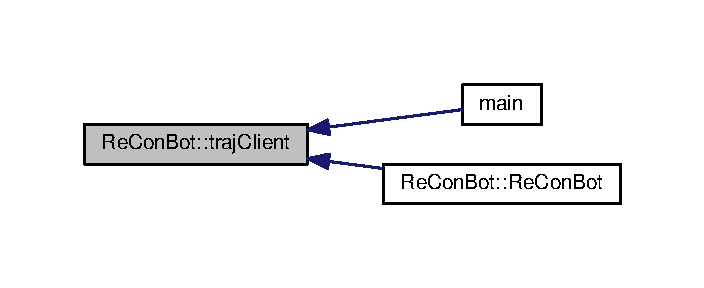
\includegraphics[width=338pt]{d9/d0b/class_re_con_bot_ab859fa96532995d3c1545aaa9db1802e_icgraph}
\end{center}
\end{figure}
\mbox{\Hypertarget{class_re_con_bot_pub_a2019b0d8d30f2419026c90dd30de500f}\label{class_re_con_bot_pub_a2019b0d8d30f2419026c90dd30de500f}} 
\index{Re\+Con\+Bot\+Pub@{Re\+Con\+Bot\+Pub}!trajectory\+Publisher\+Start@{trajectory\+Publisher\+Start}}
\index{trajectory\+Publisher\+Start@{trajectory\+Publisher\+Start}!Re\+Con\+Bot\+Pub@{Re\+Con\+Bot\+Pub}}
\subsubsection{\texorpdfstring{trajectory\+Publisher\+Start()}{trajectoryPublisherStart()}}
{\footnotesize\ttfamily void Re\+Con\+Bot\+Pub\+::trajectory\+Publisher\+Start (\begin{DoxyParamCaption}\item[{ros\+::\+Node\+Handle \&}]{nh,  }\item[{int}]{topic\+Query }\end{DoxyParamCaption})}



Definition at line 151 of file Re\+Con\+Bot.\+h.



References Re\+Con\+Bot\+::nh\+Pub, Re\+Con\+Bot\+::nh\+Pub\+\_\+pub, Re\+Con\+Bot\+::topic\+Name, and Re\+Con\+Bot\+::topic\+Query.



Referenced by main().


\begin{DoxyCode}
151                                                                            \{
152   \hyperlink{class_re_con_bot_a37edfe9c2dbbf37894c9bf850806fdd3}{nhPub} = nh;
153   \hyperlink{class_re_con_bot_a549b7542d286b690f38b7ece8b83850b}{nhPub\_pub} = \hyperlink{class_re_con_bot_a37edfe9c2dbbf37894c9bf850806fdd3}{nhPub}.advertise<control\_msgs::FollowJointTrajectoryGoal>(
      \hyperlink{class_re_con_bot_a1d91d2ea8c0f16340440357906fb9ebf}{topicName},\hyperlink{class_re_con_bot_aba20d307ac1b2e6b22f96da83a0d937d}{topicQuery});
154 \}
\end{DoxyCode}
Here is the caller graph for this function\+:\nopagebreak
\begin{figure}[H]
\begin{center}
\leavevmode
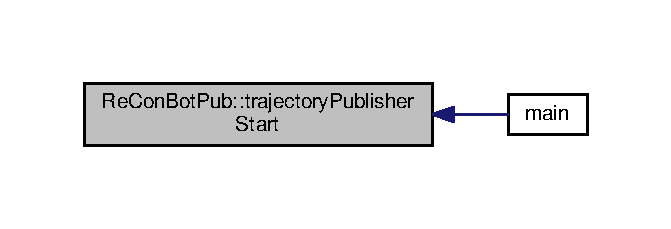
\includegraphics[width=322pt]{d6/d1b/class_re_con_bot_pub_a2019b0d8d30f2419026c90dd30de500f_icgraph}
\end{center}
\end{figure}


\subsection{Member Data Documentation}
\mbox{\Hypertarget{class_re_con_bot_pub_a2b0249f374eb7a6ab7741a85d8ebd9d5}\label{class_re_con_bot_pub_a2b0249f374eb7a6ab7741a85d8ebd9d5}} 
\index{Re\+Con\+Bot\+Pub@{Re\+Con\+Bot\+Pub}!cont@{cont}}
\index{cont@{cont}!Re\+Con\+Bot\+Pub@{Re\+Con\+Bot\+Pub}}
\subsubsection{\texorpdfstring{cont}{cont}}
{\footnotesize\ttfamily int Re\+Con\+Bot\+Pub\+::cont\hspace{0.3cm}{\ttfamily [protected]}}



Definition at line 90 of file Re\+Con\+Bot.\+h.

\mbox{\Hypertarget{class_re_con_bot_a9bd1c7ddf2376e2e68ea5d8bd8c3f505}\label{class_re_con_bot_a9bd1c7ddf2376e2e68ea5d8bd8c3f505}} 
\index{Re\+Con\+Bot\+Pub@{Re\+Con\+Bot\+Pub}!goal@{goal}}
\index{goal@{goal}!Re\+Con\+Bot\+Pub@{Re\+Con\+Bot\+Pub}}
\subsubsection{\texorpdfstring{goal}{goal}}
{\footnotesize\ttfamily control\+\_\+msgs\+::\+Follow\+Joint\+Trajectory\+Goal Re\+Con\+Bot\+::goal\hspace{0.3cm}{\ttfamily [protected]}, {\ttfamily [inherited]}}



Definition at line 60 of file Re\+Con\+Bot.\+h.



Referenced by build\+Trajectory(), Re\+Con\+Bot\+Lx\+::\+Re\+Con\+Bot\+Lx(), and Re\+Con\+Bot\+Pub().

\mbox{\Hypertarget{class_re_con_bot_pub_a1d9d82f366eeb794ffa28630de286710}\label{class_re_con_bot_pub_a1d9d82f366eeb794ffa28630de286710}} 
\index{Re\+Con\+Bot\+Pub@{Re\+Con\+Bot\+Pub}!j@{j}}
\index{j@{j}!Re\+Con\+Bot\+Pub@{Re\+Con\+Bot\+Pub}}
\subsubsection{\texorpdfstring{j}{j}}
{\footnotesize\ttfamily int Re\+Con\+Bot\+Pub\+::j\hspace{0.3cm}{\ttfamily [protected]}}



Definition at line 92 of file Re\+Con\+Bot.\+h.

\mbox{\Hypertarget{class_re_con_bot_a40ca07cd606988b78664c4a52fd8dc59}\label{class_re_con_bot_a40ca07cd606988b78664c4a52fd8dc59}} 
\index{Re\+Con\+Bot\+Pub@{Re\+Con\+Bot\+Pub}!name\+Space@{name\+Space}}
\index{name\+Space@{name\+Space}!Re\+Con\+Bot\+Pub@{Re\+Con\+Bot\+Pub}}
\subsubsection{\texorpdfstring{name\+Space}{nameSpace}}
{\footnotesize\ttfamily std\+::string Re\+Con\+Bot\+::name\+Space\hspace{0.3cm}{\ttfamily [inherited]}}



Definition at line 68 of file Re\+Con\+Bot.\+h.



Referenced by main(), and Re\+Con\+Bot\+::traj\+Client().

\mbox{\Hypertarget{class_re_con_bot_a37edfe9c2dbbf37894c9bf850806fdd3}\label{class_re_con_bot_a37edfe9c2dbbf37894c9bf850806fdd3}} 
\index{Re\+Con\+Bot\+Pub@{Re\+Con\+Bot\+Pub}!nh\+Pub@{nh\+Pub}}
\index{nh\+Pub@{nh\+Pub}!Re\+Con\+Bot\+Pub@{Re\+Con\+Bot\+Pub}}
\subsubsection{\texorpdfstring{nh\+Pub}{nhPub}}
{\footnotesize\ttfamily ros\+::\+Node\+Handle Re\+Con\+Bot\+::nh\+Pub\hspace{0.3cm}{\ttfamily [protected]}, {\ttfamily [inherited]}}



Definition at line 61 of file Re\+Con\+Bot.\+h.



Referenced by trajectory\+Publisher\+Start().

\mbox{\Hypertarget{class_re_con_bot_a549b7542d286b690f38b7ece8b83850b}\label{class_re_con_bot_a549b7542d286b690f38b7ece8b83850b}} 
\index{Re\+Con\+Bot\+Pub@{Re\+Con\+Bot\+Pub}!nh\+Pub\+\_\+pub@{nh\+Pub\+\_\+pub}}
\index{nh\+Pub\+\_\+pub@{nh\+Pub\+\_\+pub}!Re\+Con\+Bot\+Pub@{Re\+Con\+Bot\+Pub}}
\subsubsection{\texorpdfstring{nh\+Pub\+\_\+pub}{nhPub\_pub}}
{\footnotesize\ttfamily ros\+::\+Publisher Re\+Con\+Bot\+::nh\+Pub\+\_\+pub\hspace{0.3cm}{\ttfamily [protected]}, {\ttfamily [inherited]}}



Definition at line 62 of file Re\+Con\+Bot.\+h.



Referenced by publisher(), and trajectory\+Publisher\+Start().

\mbox{\Hypertarget{class_re_con_bot_pub_a51311eed78ce3a444b35924c64ad3f4c}\label{class_re_con_bot_pub_a51311eed78ce3a444b35924c64ad3f4c}} 
\index{Re\+Con\+Bot\+Pub@{Re\+Con\+Bot\+Pub}!pos@{pos}}
\index{pos@{pos}!Re\+Con\+Bot\+Pub@{Re\+Con\+Bot\+Pub}}
\subsubsection{\texorpdfstring{pos}{pos}}
{\footnotesize\ttfamily float Re\+Con\+Bot\+Pub\+::pos\hspace{0.3cm}{\ttfamily [protected]}}



Definition at line 93 of file Re\+Con\+Bot.\+h.

\mbox{\Hypertarget{class_re_con_bot_a65cf4bed9bbabd92e1265d05507e0945}\label{class_re_con_bot_a65cf4bed9bbabd92e1265d05507e0945}} 
\index{Re\+Con\+Bot\+Pub@{Re\+Con\+Bot\+Pub}!source\+File@{source\+File}}
\index{source\+File@{source\+File}!Re\+Con\+Bot\+Pub@{Re\+Con\+Bot\+Pub}}
\subsubsection{\texorpdfstring{source\+File}{sourceFile}}
{\footnotesize\ttfamily std\+::string Re\+Con\+Bot\+::source\+File\hspace{0.3cm}{\ttfamily [inherited]}}

File directory with pose data 

Definition at line 67 of file Re\+Con\+Bot.\+h.



Referenced by build\+Trajectory(), main(), and Re\+Con\+Bot\+Pub().

\mbox{\Hypertarget{class_re_con_bot_a1d91d2ea8c0f16340440357906fb9ebf}\label{class_re_con_bot_a1d91d2ea8c0f16340440357906fb9ebf}} 
\index{Re\+Con\+Bot\+Pub@{Re\+Con\+Bot\+Pub}!topic\+Name@{topic\+Name}}
\index{topic\+Name@{topic\+Name}!Re\+Con\+Bot\+Pub@{Re\+Con\+Bot\+Pub}}
\subsubsection{\texorpdfstring{topic\+Name}{topicName}}
{\footnotesize\ttfamily std\+::string Re\+Con\+Bot\+::topic\+Name\hspace{0.3cm}{\ttfamily [inherited]}}

Name given to the topic where is publishing. 

Definition at line 69 of file Re\+Con\+Bot.\+h.



Referenced by main(), Re\+Con\+Bot\+Pub(), and trajectory\+Publisher\+Start().

\mbox{\Hypertarget{class_re_con_bot_aba20d307ac1b2e6b22f96da83a0d937d}\label{class_re_con_bot_aba20d307ac1b2e6b22f96da83a0d937d}} 
\index{Re\+Con\+Bot\+Pub@{Re\+Con\+Bot\+Pub}!topic\+Query@{topic\+Query}}
\index{topic\+Query@{topic\+Query}!Re\+Con\+Bot\+Pub@{Re\+Con\+Bot\+Pub}}
\subsubsection{\texorpdfstring{topic\+Query}{topicQuery}}
{\footnotesize\ttfamily int Re\+Con\+Bot\+::topic\+Query\hspace{0.3cm}{\ttfamily [protected]}, {\ttfamily [inherited]}}



Definition at line 63 of file Re\+Con\+Bot.\+h.



Referenced by Re\+Con\+Bot\+Pub(), and trajectory\+Publisher\+Start().

\mbox{\Hypertarget{class_re_con_bot_a14a35ad6ca284af7db7228d7872720d1}\label{class_re_con_bot_a14a35ad6ca284af7db7228d7872720d1}} 
\index{Re\+Con\+Bot\+Pub@{Re\+Con\+Bot\+Pub}!traj\+\_\+client\+\_\+@{traj\+\_\+client\+\_\+}}
\index{traj\+\_\+client\+\_\+@{traj\+\_\+client\+\_\+}!Re\+Con\+Bot\+Pub@{Re\+Con\+Bot\+Pub}}
\subsubsection{\texorpdfstring{traj\+\_\+client\+\_\+}{traj\_client\_}}
{\footnotesize\ttfamily \hyperlink{basic__arm_8cpp_a6fb8875093261cdc69e54d3ac7d5c301}{Traj\+Client}$\ast$ Re\+Con\+Bot\+::traj\+\_\+client\+\_\+\hspace{0.3cm}{\ttfamily [protected]}, {\ttfamily [inherited]}}



Definition at line 59 of file Re\+Con\+Bot.\+h.



Referenced by Re\+Con\+Bot\+::get\+State(), Re\+Con\+Bot\+::start\+Trajectory(), and Re\+Con\+Bot\+::traj\+Client().

\mbox{\Hypertarget{class_re_con_bot_a7c59e136741800bf0734f659119aa5ee}\label{class_re_con_bot_a7c59e136741800bf0734f659119aa5ee}} 
\index{Re\+Con\+Bot\+Pub@{Re\+Con\+Bot\+Pub}!trajectory\+Points@{trajectory\+Points}}
\index{trajectory\+Points@{trajectory\+Points}!Re\+Con\+Bot\+Pub@{Re\+Con\+Bot\+Pub}}
\subsubsection{\texorpdfstring{trajectory\+Points}{trajectoryPoints}}
{\footnotesize\ttfamily std\+::vector$<$double$>$ Re\+Con\+Bot\+::trajectory\+Points\hspace{0.3cm}{\ttfamily [protected]}, {\ttfamily [inherited]}}



Definition at line 64 of file Re\+Con\+Bot.\+h.



Referenced by build\+Trajectory().

\mbox{\Hypertarget{class_re_con_bot_pub_ac2d5ba45905a24cfbdd78bce2dfe2a4f}\label{class_re_con_bot_pub_ac2d5ba45905a24cfbdd78bce2dfe2a4f}} 
\index{Re\+Con\+Bot\+Pub@{Re\+Con\+Bot\+Pub}!var@{var}}
\index{var@{var}!Re\+Con\+Bot\+Pub@{Re\+Con\+Bot\+Pub}}
\subsubsection{\texorpdfstring{var}{var}}
{\footnotesize\ttfamily int Re\+Con\+Bot\+Pub\+::var\hspace{0.3cm}{\ttfamily [protected]}}



Definition at line 91 of file Re\+Con\+Bot.\+h.



The documentation for this class was generated from the following file\+:\begin{DoxyCompactItemize}
\item 
\hyperlink{_re_con_bot_8h}{Re\+Con\+Bot.\+h}\end{DoxyCompactItemize}

\chapter{File Documentation}
\hypertarget{basic__arm_8cpp}{}\section{basic\+\_\+arm.\+cpp File Reference}
\label{basic__arm_8cpp}\index{basic\+\_\+arm.\+cpp@{basic\+\_\+arm.\+cpp}}
{\ttfamily \#include $<$ros/ros.\+h$>$}\newline
{\ttfamily \#include $<$control\+\_\+msgs/\+Follow\+Joint\+Trajectory\+Action.\+h$>$}\newline
{\ttfamily \#include $<$actionlib/client/simple\+\_\+action\+\_\+client.\+h$>$}\newline
Include dependency graph for basic\+\_\+arm.\+cpp\+:\nopagebreak
\begin{figure}[H]
\begin{center}
\leavevmode
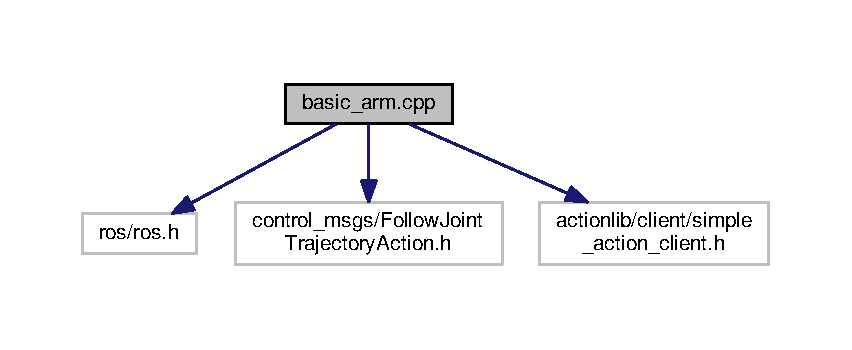
\includegraphics[width=350pt]{d2/d5f/basic__arm_8cpp__incl}
\end{center}
\end{figure}
\subsection*{Classes}
\begin{DoxyCompactItemize}
\item 
class \hyperlink{class_re_con_bot_arm}{Re\+Con\+Bot\+Arm}
\end{DoxyCompactItemize}
\subsection*{Typedefs}
\begin{DoxyCompactItemize}
\item 
typedef actionlib\+::\+Simple\+Action\+Client$<$ control\+\_\+msgs\+::\+Follow\+Joint\+Trajectory\+Action $>$ \hyperlink{basic__arm_8cpp_a6fb8875093261cdc69e54d3ac7d5c301}{Traj\+Client}
\end{DoxyCompactItemize}
\subsection*{Functions}
\begin{DoxyCompactItemize}
\item 
int \hyperlink{basic__arm_8cpp_a3c04138a5bfe5d72780bb7e82a18e627}{main} (int argc, char $\ast$$\ast$argv)
\end{DoxyCompactItemize}


\subsection{Typedef Documentation}
\mbox{\Hypertarget{basic__arm_8cpp_a6fb8875093261cdc69e54d3ac7d5c301}\label{basic__arm_8cpp_a6fb8875093261cdc69e54d3ac7d5c301}} 
\index{basic\+\_\+arm.\+cpp@{basic\+\_\+arm.\+cpp}!Traj\+Client@{Traj\+Client}}
\index{Traj\+Client@{Traj\+Client}!basic\+\_\+arm.\+cpp@{basic\+\_\+arm.\+cpp}}
\subsubsection{\texorpdfstring{Traj\+Client}{TrajClient}}
{\footnotesize\ttfamily typedef actionlib\+::\+Simple\+Action\+Client$<$control\+\_\+msgs\+::\+Follow\+Joint\+Trajectory\+Action$>$ \hyperlink{basic__arm_8cpp_a6fb8875093261cdc69e54d3ac7d5c301}{Traj\+Client}}

\begin{DoxyAuthor}{Author}
Jorge De La Cruz 
\end{DoxyAuthor}
\begin{DoxyVersion}{Version}
1.\+0 
\end{DoxyVersion}
\begin{DoxyDate}{Date}
February 20, 2017 
\end{DoxyDate}


Definition at line 45 of file basic\+\_\+arm.\+cpp.



\subsection{Function Documentation}
\mbox{\Hypertarget{basic__arm_8cpp_a3c04138a5bfe5d72780bb7e82a18e627}\label{basic__arm_8cpp_a3c04138a5bfe5d72780bb7e82a18e627}} 
\index{basic\+\_\+arm.\+cpp@{basic\+\_\+arm.\+cpp}!main@{main}}
\index{main@{main}!basic\+\_\+arm.\+cpp@{basic\+\_\+arm.\+cpp}}
\subsubsection{\texorpdfstring{main()}{main()}}
{\footnotesize\ttfamily int main (\begin{DoxyParamCaption}\item[{int}]{argc,  }\item[{char $\ast$$\ast$}]{argv }\end{DoxyParamCaption})}



Definition at line 146 of file basic\+\_\+arm.\+cpp.



References Re\+Con\+Bot\+Arm\+::arm\+Trajectory(), Re\+Con\+Bot\+Arm\+::get\+State(), and Re\+Con\+Bot\+Arm\+::start\+Trajectory().


\begin{DoxyCode}
147 \{
148   \textcolor{comment}{// Init the ROS node}
149   ros::init(argc, argv, \textcolor{stringliteral}{"ReConBot\_Driver"});
150 
151   \hyperlink{class_re_con_bot_arm}{ReConBotArm} arm;
152   \textcolor{comment}{// Start the trajectory}
153   arm.\hyperlink{class_re_con_bot_arm_a52f6f89615b17a421d5cd8b51b2962d7}{startTrajectory}(arm.\hyperlink{class_re_con_bot_arm_ac499ee22d73b90c860f06a16afcd2fb0}{armTrajectory}());
154   \textcolor{comment}{// Wait for trajectory completion}
155   \textcolor{keywordflow}{while}(!arm.\hyperlink{class_re_con_bot_arm_a179480efa62ff256fb8b3ddc0685d762}{getState}().isDone() && ros::ok())
156   \{
157     usleep(8000000);
158   \}
159 \}
\end{DoxyCode}
Here is the call graph for this function\+:\nopagebreak
\begin{figure}[H]
\begin{center}
\leavevmode
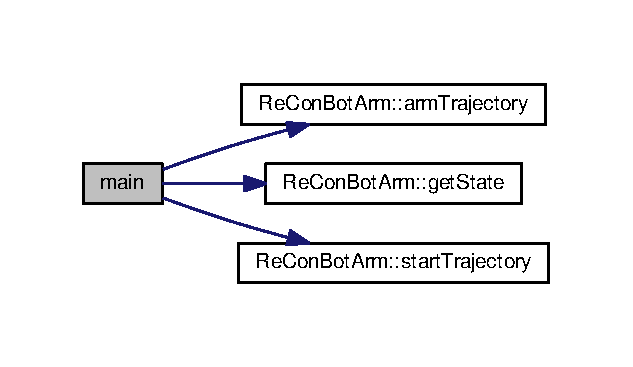
\includegraphics[width=304pt]{d5/d2d/basic__arm_8cpp_a3c04138a5bfe5d72780bb7e82a18e627_cgraph}
\end{center}
\end{figure}

\hypertarget{l__arm__move__group__interface_8cpp}{}\section{l\+\_\+arm\+\_\+move\+\_\+group\+\_\+interface.\+cpp File Reference}
\label{l__arm__move__group__interface_8cpp}\index{l\+\_\+arm\+\_\+move\+\_\+group\+\_\+interface.\+cpp@{l\+\_\+arm\+\_\+move\+\_\+group\+\_\+interface.\+cpp}}
{\ttfamily \#include $<$ros/ros.\+h$>$}\newline
{\ttfamily \#include $<$control\+\_\+msgs/\+Follow\+Joint\+Trajectory\+Action.\+h$>$}\newline
{\ttfamily \#include $<$actionlib/client/simple\+\_\+action\+\_\+client.\+h$>$}\newline
{\ttfamily \#include $<$iostream$>$}\newline
{\ttfamily \#include $<$fstream$>$}\newline
{\ttfamily \#include $<$string$>$}\newline
{\ttfamily \#include $<$vector$>$}\newline
{\ttfamily \#include \char`\"{}Re\+Con\+Bot.\+h\char`\"{}}\newline
Include dependency graph for l\+\_\+arm\+\_\+move\+\_\+group\+\_\+interface.\+cpp\+:\nopagebreak
\begin{figure}[H]
\begin{center}
\leavevmode
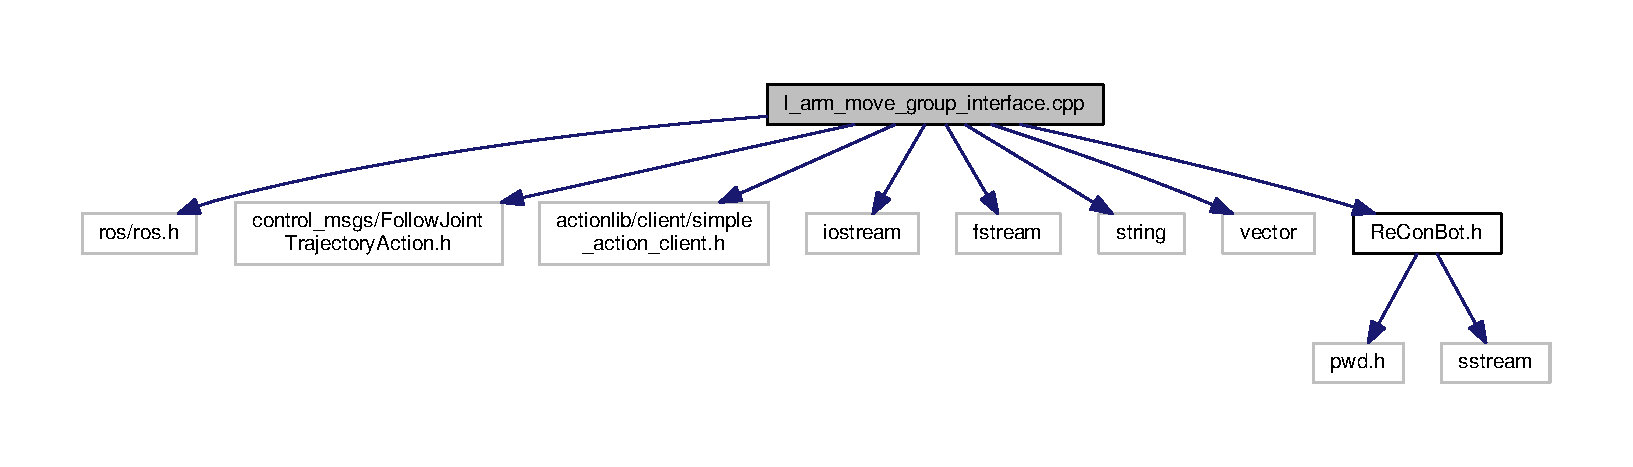
\includegraphics[width=350pt]{d6/d79/l__arm__move__group__interface_8cpp__incl}
\end{center}
\end{figure}
\subsection*{Functions}
\begin{DoxyCompactItemize}
\item 
int \hyperlink{l__arm__move__group__interface_8cpp_a3c04138a5bfe5d72780bb7e82a18e627}{main} (int argc, char $\ast$$\ast$argv)
\end{DoxyCompactItemize}


\subsection{Function Documentation}
\mbox{\Hypertarget{l__arm__move__group__interface_8cpp_a3c04138a5bfe5d72780bb7e82a18e627}\label{l__arm__move__group__interface_8cpp_a3c04138a5bfe5d72780bb7e82a18e627}} 
\index{l\+\_\+arm\+\_\+move\+\_\+group\+\_\+interface.\+cpp@{l\+\_\+arm\+\_\+move\+\_\+group\+\_\+interface.\+cpp}!main@{main}}
\index{main@{main}!l\+\_\+arm\+\_\+move\+\_\+group\+\_\+interface.\+cpp@{l\+\_\+arm\+\_\+move\+\_\+group\+\_\+interface.\+cpp}}
\subsubsection{\texorpdfstring{main()}{main()}}
{\footnotesize\ttfamily int main (\begin{DoxyParamCaption}\item[{int}]{argc,  }\item[{char $\ast$$\ast$}]{argv }\end{DoxyParamCaption})}

\begin{DoxyAuthor}{Author}
Jorge De La Cruz 
\end{DoxyAuthor}
\begin{DoxyVersion}{Version}
1.\+0 
\end{DoxyVersion}
\begin{DoxyDate}{Date}
February 20, 2017 
\end{DoxyDate}


Definition at line 50 of file l\+\_\+arm\+\_\+move\+\_\+group\+\_\+interface.\+cpp.



References Re\+Con\+Bot\+::name\+Space, Re\+Con\+Bot\+Lx\+::reconbot\+Callback(), and Re\+Con\+Bot\+::traj\+Client().


\begin{DoxyCode}
51 \{
52   \textcolor{comment}{// Init the ROS node}
53   ros::init(argc, argv, \textcolor{stringliteral}{"l\_arm\_ReConBot\_Driver"});
54   ros::NodeHandle nh\_;
55   ros::Subscriber sub\_path;
56   \hyperlink{class_re_con_bot_lx}{ReConBotLx} Robot;
57   Robot.\hyperlink{class_re_con_bot_a40ca07cd606988b78664c4a52fd8dc59}{nameSpace} = \textcolor{stringliteral}{"l\_arm\_reconbot\_controller"};
58   Robot.\hyperlink{class_re_con_bot_ab859fa96532995d3c1545aaa9db1802e}{trajClient}();
59 
60   sub\_path = nh\_.subscribe(\textcolor{stringliteral}{"/l\_arm\_reconbot\_trajectory"}, 100, &
      \hyperlink{class_re_con_bot_lx_a5d60b16962e5ce8e452f7c53543c54ce}{ReConBotLx::reconbotCallback}, &Robot);
61   \textcolor{comment}{// Start the trajectory}
62   \textcolor{comment}{// Wait for trajectory completion}
63   \textcolor{comment}{//while(!robot.getState().isDone() && ros::ok())}
64   \textcolor{comment}{//\{}
65   \textcolor{comment}{//  usleep(50000);}
66   \textcolor{comment}{//\}}
67   sleep(8);
68   ros::spin();
69 \}
\end{DoxyCode}
Here is the call graph for this function\+:\nopagebreak
\begin{figure}[H]
\begin{center}
\leavevmode
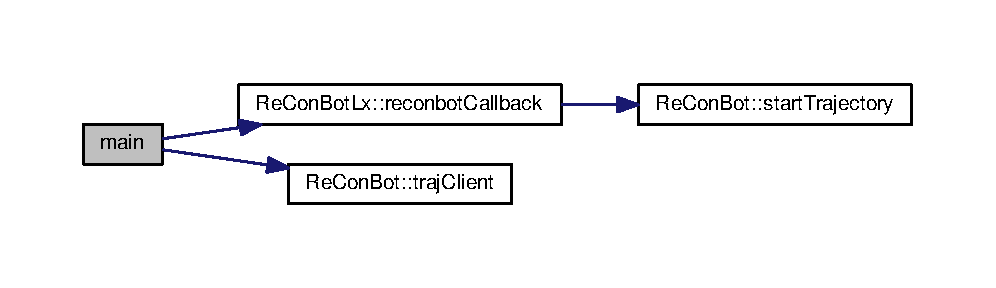
\includegraphics[width=350pt]{df/d92/l__arm__move__group__interface_8cpp_a3c04138a5bfe5d72780bb7e82a18e627_cgraph}
\end{center}
\end{figure}

\hypertarget{l__arm__trajectory__publisher_8cpp}{}\section{l\+\_\+arm\+\_\+trajectory\+\_\+publisher.\+cpp File Reference}
\label{l__arm__trajectory__publisher_8cpp}\index{l\+\_\+arm\+\_\+trajectory\+\_\+publisher.\+cpp@{l\+\_\+arm\+\_\+trajectory\+\_\+publisher.\+cpp}}
{\ttfamily \#include $<$ros/ros.\+h$>$}\newline
{\ttfamily \#include $<$control\+\_\+msgs/\+Follow\+Joint\+Trajectory\+Action.\+h$>$}\newline
{\ttfamily \#include $<$actionlib/client/simple\+\_\+action\+\_\+client.\+h$>$}\newline
{\ttfamily \#include $<$iostream$>$}\newline
{\ttfamily \#include $<$fstream$>$}\newline
{\ttfamily \#include \char`\"{}Re\+Con\+Bot.\+h\char`\"{}}\newline
{\ttfamily \#include $<$string$>$}\newline
{\ttfamily \#include $<$vector$>$}\newline
{\ttfamily \#include $<$cstdlib$>$}\newline
{\ttfamily \#include $<$map$>$}\newline
{\ttfamily \#include $<$pwd.\+h$>$}\newline
Include dependency graph for l\+\_\+arm\+\_\+trajectory\+\_\+publisher.\+cpp\+:\nopagebreak
\begin{figure}[H]
\begin{center}
\leavevmode
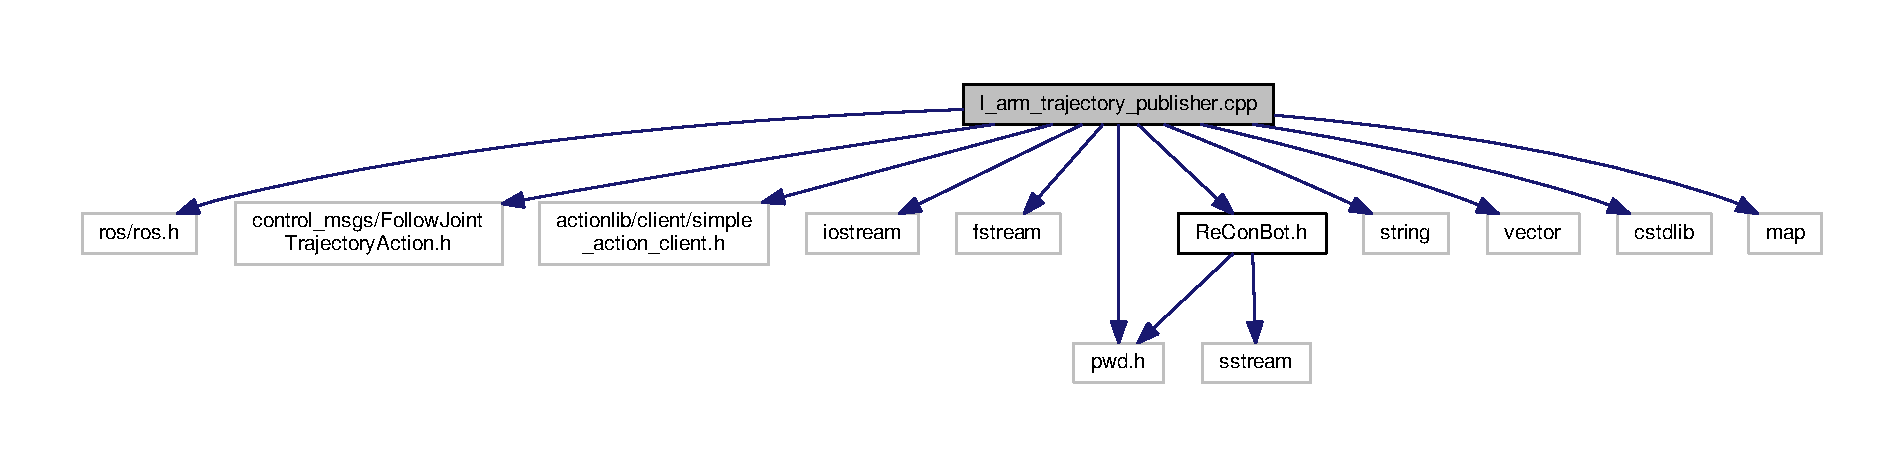
\includegraphics[width=350pt]{d6/da2/l__arm__trajectory__publisher_8cpp__incl}
\end{center}
\end{figure}
\subsection*{Functions}
\begin{DoxyCompactItemize}
\item 
int \hyperlink{l__arm__trajectory__publisher_8cpp_a3c04138a5bfe5d72780bb7e82a18e627}{main} (int argc, char $\ast$$\ast$argv)
\end{DoxyCompactItemize}


\subsection{Function Documentation}
\mbox{\Hypertarget{l__arm__trajectory__publisher_8cpp_a3c04138a5bfe5d72780bb7e82a18e627}\label{l__arm__trajectory__publisher_8cpp_a3c04138a5bfe5d72780bb7e82a18e627}} 
\index{l\+\_\+arm\+\_\+trajectory\+\_\+publisher.\+cpp@{l\+\_\+arm\+\_\+trajectory\+\_\+publisher.\+cpp}!main@{main}}
\index{main@{main}!l\+\_\+arm\+\_\+trajectory\+\_\+publisher.\+cpp@{l\+\_\+arm\+\_\+trajectory\+\_\+publisher.\+cpp}}
\subsubsection{\texorpdfstring{main()}{main()}}
{\footnotesize\ttfamily int main (\begin{DoxyParamCaption}\item[{int}]{argc,  }\item[{char $\ast$$\ast$}]{argv }\end{DoxyParamCaption})}



Definition at line 15 of file l\+\_\+arm\+\_\+trajectory\+\_\+publisher.\+cpp.



References Re\+Con\+Bot\+Pub\+::build\+Trajectory(), Re\+Con\+Bot\+Lx\+::motors\+State(), Re\+Con\+Bot\+::name\+Space, Re\+Con\+Bot\+Pub\+::publisher(), Re\+Con\+Bot\+::source\+File, Re\+Con\+Bot\+::topic\+Name, and Re\+Con\+Bot\+Pub\+::trajectory\+Publisher\+Start().


\begin{DoxyCode}
15                               \{
16   ros::init(argc, argv, \textcolor{stringliteral}{"l\_arm\_Trajectory\_Publisher"});
17   ros::NodeHandle nh;
18   control\_msgs::FollowJointTrajectoryGoal goal;
19   \textcolor{comment}{//ros::Rate loop\_rate(5);}
20   \textcolor{comment}{//ros::AsyncSpinner spinner(1);/**<Two spinner are instantiated for managing 2 threats*/}
21   \textcolor{comment}{//spinner.start();}
22   \hyperlink{class_re_con_bot_pub}{ReConBotPub} Publisher;
23   Publisher.\hyperlink{class_re_con_bot_a1d91d2ea8c0f16340440357906fb9ebf}{topicName} = \textcolor{stringliteral}{"/l\_arm\_reconbot\_trajectory"};
24   \textcolor{keywordtype}{int} arg[] = \{4,5,6\};
25 
26   passwd* pw = getpwuid(getuid());
27   std::string path(pw->pw\_dir);
28 
29   Publisher.\hyperlink{class_re_con_bot_lx_a0e25f573057755c6729ea572362652e6}{motorsState}(arg,3);
30   Publisher.\hyperlink{class_re_con_bot_pub_a2019b0d8d30f2419026c90dd30de500f}{trajectoryPublisherStart}(nh, 1000);
31   Publisher.\hyperlink{class_re_con_bot_a40ca07cd606988b78664c4a52fd8dc59}{nameSpace} = \textcolor{stringliteral}{"l\_arm\_reconbot\_controller"};
32   Publisher.\hyperlink{class_re_con_bot_a65cf4bed9bbabd92e1265d05507e0945}{sourceFile} = path += \textcolor{stringliteral}{"/catkin\_ws/src/reconbot/trajectory/l\_arm\_trajectory.txt"};
33   goal = Publisher.\hyperlink{class_re_con_bot_pub_af99f5189cd8e834d7b59f1b106b99345}{buildTrajectory}();
34   Publisher.\hyperlink{class_re_con_bot_pub_ac763949cb5256de695e02c5f81084ead}{publisher}(goal);
35 
36   sleep(3);
37 
38   ROS\_INFO(\textcolor{stringliteral}{"Good bye!"});
39   \textcolor{comment}{//spinner.stop();}
40   \textcolor{comment}{//loop\_rate.sleep();}
41 
42   \textcolor{comment}{//sleep(2);}
43   \textcolor{keywordflow}{return} 0;
44 \}
\end{DoxyCode}
Here is the call graph for this function\+:\nopagebreak
\begin{figure}[H]
\begin{center}
\leavevmode
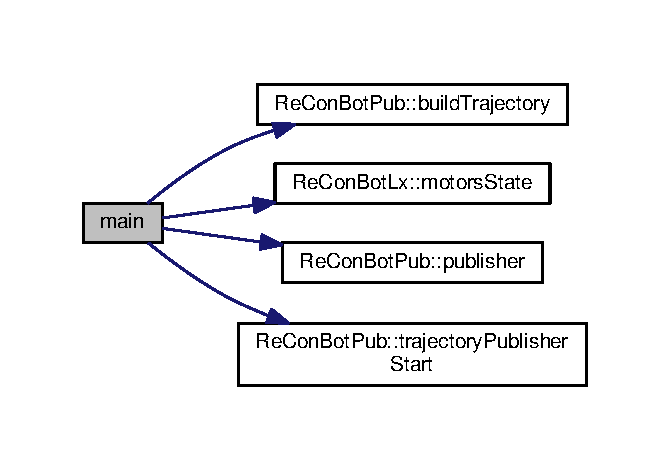
\includegraphics[width=322pt]{d8/d54/l__arm__trajectory__publisher_8cpp_a3c04138a5bfe5d72780bb7e82a18e627_cgraph}
\end{center}
\end{figure}

\hypertarget{main_8md}{}\section{main.\+md File Reference}
\label{main_8md}\index{main.\+md@{main.\+md}}

\hypertarget{move__group__interface_8cpp}{}\section{move\+\_\+group\+\_\+interface.\+cpp File Reference}
\label{move__group__interface_8cpp}\index{move\+\_\+group\+\_\+interface.\+cpp@{move\+\_\+group\+\_\+interface.\+cpp}}
{\ttfamily \#include $<$ros/ros.\+h$>$}\newline
{\ttfamily \#include $<$control\+\_\+msgs/\+Follow\+Joint\+Trajectory\+Action.\+h$>$}\newline
{\ttfamily \#include $<$actionlib/client/simple\+\_\+action\+\_\+client.\+h$>$}\newline
{\ttfamily \#include $<$iostream$>$}\newline
{\ttfamily \#include $<$fstream$>$}\newline
{\ttfamily \#include $<$string$>$}\newline
{\ttfamily \#include $<$vector$>$}\newline
{\ttfamily \#include \char`\"{}Re\+Con\+Bot.\+h\char`\"{}}\newline
Include dependency graph for move\+\_\+group\+\_\+interface.\+cpp\+:\nopagebreak
\begin{figure}[H]
\begin{center}
\leavevmode
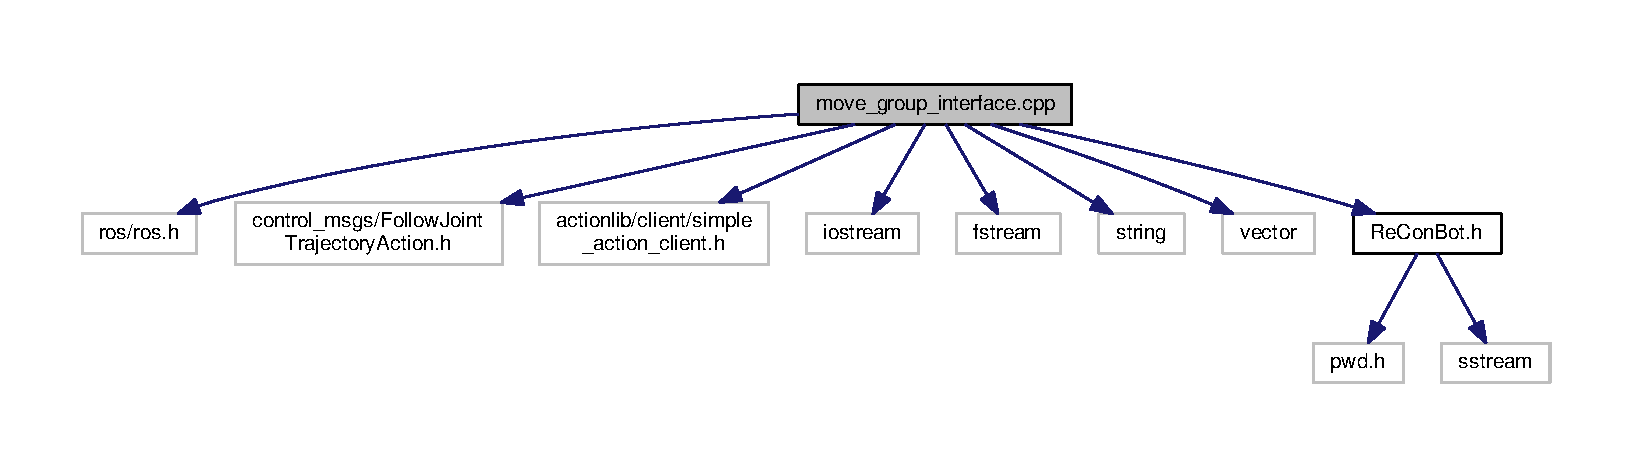
\includegraphics[width=350pt]{d7/d0b/move__group__interface_8cpp__incl}
\end{center}
\end{figure}
\subsection*{Functions}
\begin{DoxyCompactItemize}
\item 
int \hyperlink{move__group__interface_8cpp_a3c04138a5bfe5d72780bb7e82a18e627}{main} (int argc, char $\ast$$\ast$argv)
\end{DoxyCompactItemize}


\subsection{Function Documentation}
\mbox{\Hypertarget{move__group__interface_8cpp_a3c04138a5bfe5d72780bb7e82a18e627}\label{move__group__interface_8cpp_a3c04138a5bfe5d72780bb7e82a18e627}} 
\index{move\+\_\+group\+\_\+interface.\+cpp@{move\+\_\+group\+\_\+interface.\+cpp}!main@{main}}
\index{main@{main}!move\+\_\+group\+\_\+interface.\+cpp@{move\+\_\+group\+\_\+interface.\+cpp}}
\subsubsection{\texorpdfstring{main()}{main()}}
{\footnotesize\ttfamily int main (\begin{DoxyParamCaption}\item[{int}]{argc,  }\item[{char $\ast$$\ast$}]{argv }\end{DoxyParamCaption})}

\begin{DoxyAuthor}{Author}
Jorge De La Cruz 
\end{DoxyAuthor}
\begin{DoxyVersion}{Version}
1.\+0 
\end{DoxyVersion}
\begin{DoxyDate}{Date}
February 20, 2017 
\end{DoxyDate}


Definition at line 50 of file move\+\_\+group\+\_\+interface.\+cpp.



References Re\+Con\+Bot\+::name\+Space, Re\+Con\+Bot\+Lx\+::reconbot\+Callback(), and Re\+Con\+Bot\+::traj\+Client().


\begin{DoxyCode}
51 \{
52   \textcolor{comment}{// Init the ROS node}
53   ros::init(argc, argv, \textcolor{stringliteral}{"ReConBot\_Driver"});
54   ros::NodeHandle nh\_;
55   ros::Subscriber sub\_path;
56   \hyperlink{class_re_con_bot_lx}{ReConBotLx} Robot;
57   Robot.\hyperlink{class_re_con_bot_a40ca07cd606988b78664c4a52fd8dc59}{nameSpace} = \textcolor{stringliteral}{"reconbot\_controller"};
58   Robot.\hyperlink{class_re_con_bot_ab859fa96532995d3c1545aaa9db1802e}{trajClient}();
59 
60   sub\_path = nh\_.subscribe(\textcolor{stringliteral}{"/reconbot\_trajectory"}, 100, &
      \hyperlink{class_re_con_bot_lx_a5d60b16962e5ce8e452f7c53543c54ce}{ReConBotLx::reconbotCallback}, &Robot);
61   \textcolor{comment}{// Start the trajectory}
62   \textcolor{comment}{// Wait for trajectory completion}
63   \textcolor{comment}{//while(!robot.getState().isDone() && ros::ok())}
64   \textcolor{comment}{//\{}
65   \textcolor{comment}{//  usleep(50000);}
66   \textcolor{comment}{//\}}
67   sleep(8);
68   ros::spin();
69 \}
\end{DoxyCode}
Here is the call graph for this function\+:\nopagebreak
\begin{figure}[H]
\begin{center}
\leavevmode
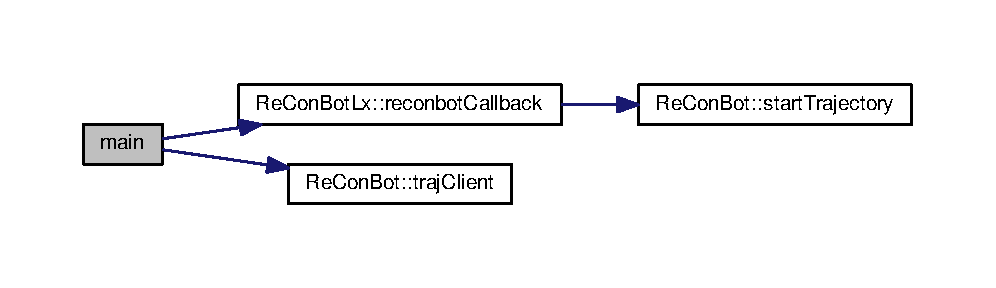
\includegraphics[width=350pt]{d5/d6c/move__group__interface_8cpp_a3c04138a5bfe5d72780bb7e82a18e627_cgraph}
\end{center}
\end{figure}

\hypertarget{r__arm__move__group__interface_8cpp}{}\section{r\+\_\+arm\+\_\+move\+\_\+group\+\_\+interface.\+cpp File Reference}
\label{r__arm__move__group__interface_8cpp}\index{r\+\_\+arm\+\_\+move\+\_\+group\+\_\+interface.\+cpp@{r\+\_\+arm\+\_\+move\+\_\+group\+\_\+interface.\+cpp}}
{\ttfamily \#include $<$ros/ros.\+h$>$}\newline
{\ttfamily \#include $<$control\+\_\+msgs/\+Follow\+Joint\+Trajectory\+Action.\+h$>$}\newline
{\ttfamily \#include $<$actionlib/client/simple\+\_\+action\+\_\+client.\+h$>$}\newline
{\ttfamily \#include $<$iostream$>$}\newline
{\ttfamily \#include $<$fstream$>$}\newline
{\ttfamily \#include $<$string$>$}\newline
{\ttfamily \#include $<$vector$>$}\newline
{\ttfamily \#include \char`\"{}Re\+Con\+Bot.\+h\char`\"{}}\newline
Include dependency graph for r\+\_\+arm\+\_\+move\+\_\+group\+\_\+interface.\+cpp\+:\nopagebreak
\begin{figure}[H]
\begin{center}
\leavevmode
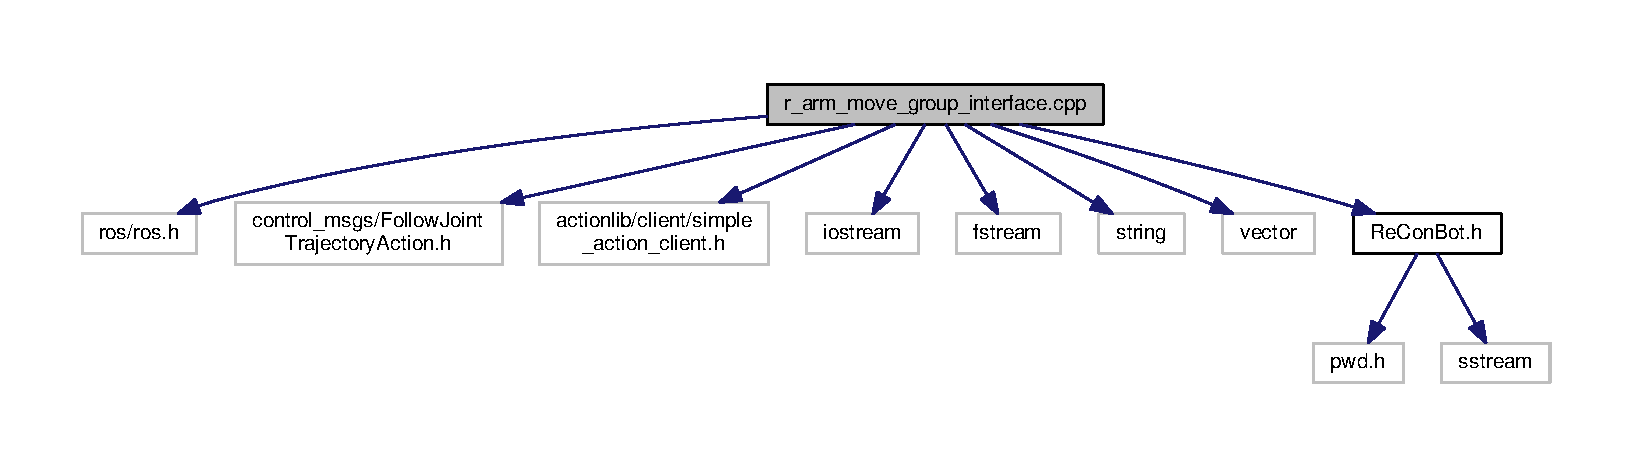
\includegraphics[width=350pt]{dc/df0/r__arm__move__group__interface_8cpp__incl}
\end{center}
\end{figure}
\subsection*{Functions}
\begin{DoxyCompactItemize}
\item 
int \hyperlink{r__arm__move__group__interface_8cpp_a3c04138a5bfe5d72780bb7e82a18e627}{main} (int argc, char $\ast$$\ast$argv)
\end{DoxyCompactItemize}


\subsection{Function Documentation}
\mbox{\Hypertarget{r__arm__move__group__interface_8cpp_a3c04138a5bfe5d72780bb7e82a18e627}\label{r__arm__move__group__interface_8cpp_a3c04138a5bfe5d72780bb7e82a18e627}} 
\index{r\+\_\+arm\+\_\+move\+\_\+group\+\_\+interface.\+cpp@{r\+\_\+arm\+\_\+move\+\_\+group\+\_\+interface.\+cpp}!main@{main}}
\index{main@{main}!r\+\_\+arm\+\_\+move\+\_\+group\+\_\+interface.\+cpp@{r\+\_\+arm\+\_\+move\+\_\+group\+\_\+interface.\+cpp}}
\subsubsection{\texorpdfstring{main()}{main()}}
{\footnotesize\ttfamily int main (\begin{DoxyParamCaption}\item[{int}]{argc,  }\item[{char $\ast$$\ast$}]{argv }\end{DoxyParamCaption})}

\begin{DoxyAuthor}{Author}
Jorge De La Cruz 
\end{DoxyAuthor}
\begin{DoxyVersion}{Version}
1.\+0 
\end{DoxyVersion}
\begin{DoxyDate}{Date}
February 20, 2017 
\end{DoxyDate}


Definition at line 50 of file r\+\_\+arm\+\_\+move\+\_\+group\+\_\+interface.\+cpp.



References Re\+Con\+Bot\+::name\+Space, Re\+Con\+Bot\+Lx\+::reconbot\+Callback(), and Re\+Con\+Bot\+::traj\+Client().


\begin{DoxyCode}
51 \{
52   \textcolor{comment}{// Init the ROS node}
53   ros::init(argc, argv, \textcolor{stringliteral}{"r\_arm\_ReConBot\_Driver"});
54   ros::NodeHandle nh\_;
55   ros::Subscriber sub\_path;
56   \hyperlink{class_re_con_bot_lx}{ReConBotLx} Robot;
57   Robot.\hyperlink{class_re_con_bot_a40ca07cd606988b78664c4a52fd8dc59}{nameSpace} = \textcolor{stringliteral}{"r\_arm\_reconbot\_controller"};
58   Robot.\hyperlink{class_re_con_bot_ab859fa96532995d3c1545aaa9db1802e}{trajClient}();
59 
60   sub\_path = nh\_.subscribe(\textcolor{stringliteral}{"/r\_arm\_reconbot\_trajectory"}, 100, &
      \hyperlink{class_re_con_bot_lx_a5d60b16962e5ce8e452f7c53543c54ce}{ReConBotLx::reconbotCallback}, &Robot);
61   \textcolor{comment}{// Start the trajectory}
62   \textcolor{comment}{// Wait for trajectory completion}
63   \textcolor{comment}{//while(!robot.getState().isDone() && ros::ok())}
64   \textcolor{comment}{//\{}
65   \textcolor{comment}{//  usleep(50000);}
66   \textcolor{comment}{//\}}
67   sleep(8);
68   ros::spin();
69 \}
\end{DoxyCode}
Here is the call graph for this function\+:\nopagebreak
\begin{figure}[H]
\begin{center}
\leavevmode
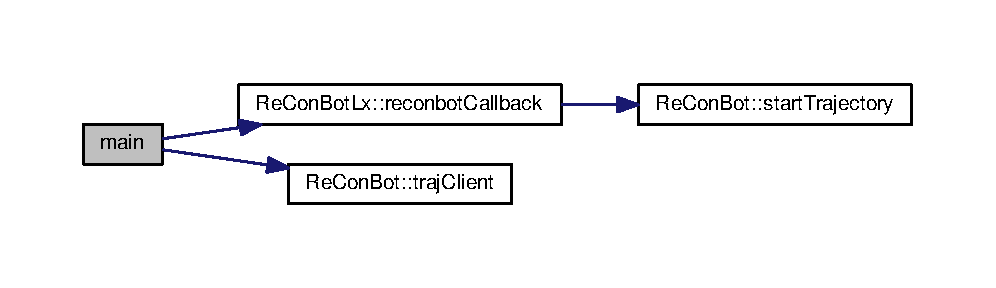
\includegraphics[width=350pt]{d9/dd4/r__arm__move__group__interface_8cpp_a3c04138a5bfe5d72780bb7e82a18e627_cgraph}
\end{center}
\end{figure}

\hypertarget{r__arm__trajectory__publisher_8cpp}{}\section{r\+\_\+arm\+\_\+trajectory\+\_\+publisher.\+cpp File Reference}
\label{r__arm__trajectory__publisher_8cpp}\index{r\+\_\+arm\+\_\+trajectory\+\_\+publisher.\+cpp@{r\+\_\+arm\+\_\+trajectory\+\_\+publisher.\+cpp}}
{\ttfamily \#include $<$ros/ros.\+h$>$}\newline
{\ttfamily \#include $<$control\+\_\+msgs/\+Follow\+Joint\+Trajectory\+Action.\+h$>$}\newline
{\ttfamily \#include $<$actionlib/client/simple\+\_\+action\+\_\+client.\+h$>$}\newline
{\ttfamily \#include $<$iostream$>$}\newline
{\ttfamily \#include $<$fstream$>$}\newline
{\ttfamily \#include \char`\"{}Re\+Con\+Bot.\+h\char`\"{}}\newline
{\ttfamily \#include $<$string$>$}\newline
{\ttfamily \#include $<$vector$>$}\newline
{\ttfamily \#include $<$cstdlib$>$}\newline
{\ttfamily \#include $<$map$>$}\newline
{\ttfamily \#include $<$pwd.\+h$>$}\newline
Include dependency graph for r\+\_\+arm\+\_\+trajectory\+\_\+publisher.\+cpp\+:\nopagebreak
\begin{figure}[H]
\begin{center}
\leavevmode
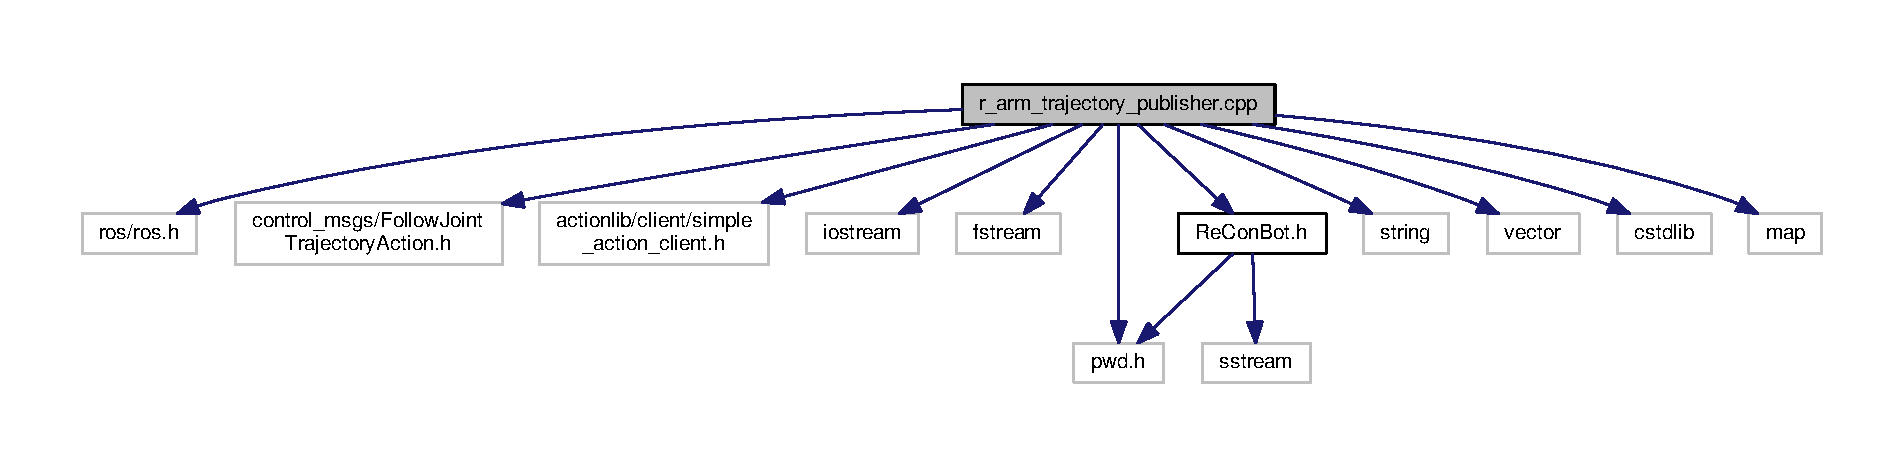
\includegraphics[width=350pt]{d7/d13/r__arm__trajectory__publisher_8cpp__incl}
\end{center}
\end{figure}
\subsection*{Functions}
\begin{DoxyCompactItemize}
\item 
int \hyperlink{r__arm__trajectory__publisher_8cpp_a3c04138a5bfe5d72780bb7e82a18e627}{main} (int argc, char $\ast$$\ast$argv)
\end{DoxyCompactItemize}


\subsection{Function Documentation}
\mbox{\Hypertarget{r__arm__trajectory__publisher_8cpp_a3c04138a5bfe5d72780bb7e82a18e627}\label{r__arm__trajectory__publisher_8cpp_a3c04138a5bfe5d72780bb7e82a18e627}} 
\index{r\+\_\+arm\+\_\+trajectory\+\_\+publisher.\+cpp@{r\+\_\+arm\+\_\+trajectory\+\_\+publisher.\+cpp}!main@{main}}
\index{main@{main}!r\+\_\+arm\+\_\+trajectory\+\_\+publisher.\+cpp@{r\+\_\+arm\+\_\+trajectory\+\_\+publisher.\+cpp}}
\subsubsection{\texorpdfstring{main()}{main()}}
{\footnotesize\ttfamily int main (\begin{DoxyParamCaption}\item[{int}]{argc,  }\item[{char $\ast$$\ast$}]{argv }\end{DoxyParamCaption})}



Definition at line 15 of file r\+\_\+arm\+\_\+trajectory\+\_\+publisher.\+cpp.



References Re\+Con\+Bot\+Pub\+::build\+Trajectory(), Re\+Con\+Bot\+Lx\+::motors\+State(), Re\+Con\+Bot\+::name\+Space, Re\+Con\+Bot\+Pub\+::publisher(), Re\+Con\+Bot\+::source\+File, Re\+Con\+Bot\+::topic\+Name, and Re\+Con\+Bot\+Pub\+::trajectory\+Publisher\+Start().


\begin{DoxyCode}
15                               \{
16   ros::init(argc, argv, \textcolor{stringliteral}{"r\_arm\_Trajectory\_Publisher"});
17   ros::NodeHandle nh;
18   control\_msgs::FollowJointTrajectoryGoal goal;
19   \textcolor{comment}{//ros::Rate loop\_rate(5);}
20   \textcolor{comment}{//ros::AsyncSpinner spinner(1);/**<Two spinner are instantiated for managing 2 threats*/}
21   \textcolor{comment}{//spinner.start();}
22   \hyperlink{class_re_con_bot_pub}{ReConBotPub} Publisher;
23   Publisher.\hyperlink{class_re_con_bot_a1d91d2ea8c0f16340440357906fb9ebf}{topicName} = \textcolor{stringliteral}{"/r\_arm\_reconbot\_trajectory"};
24   \textcolor{keywordtype}{int} arg[] = \{1,2,3\};
25 
26   passwd* pw = getpwuid(getuid());
27   std::string path(pw->pw\_dir);
28 
29   Publisher.\hyperlink{class_re_con_bot_lx_a0e25f573057755c6729ea572362652e6}{motorsState}(arg,3);
30   Publisher.\hyperlink{class_re_con_bot_pub_a2019b0d8d30f2419026c90dd30de500f}{trajectoryPublisherStart}(nh, 1000);
31   Publisher.\hyperlink{class_re_con_bot_a40ca07cd606988b78664c4a52fd8dc59}{nameSpace} = \textcolor{stringliteral}{"r\_arm\_reconbot\_controller"};
32   Publisher.\hyperlink{class_re_con_bot_a65cf4bed9bbabd92e1265d05507e0945}{sourceFile} = path += \textcolor{stringliteral}{"/catkin\_ws/src/reconbot/trajectory/r\_arm\_trajectory.txt"};
33   goal = Publisher.\hyperlink{class_re_con_bot_pub_af99f5189cd8e834d7b59f1b106b99345}{buildTrajectory}();
34   Publisher.\hyperlink{class_re_con_bot_pub_ac763949cb5256de695e02c5f81084ead}{publisher}(goal);
35 
36   sleep(3);
37 
38   ROS\_INFO(\textcolor{stringliteral}{"Good bye!"});
39   \textcolor{comment}{//spinner.stop();}
40   \textcolor{comment}{//loop\_rate.sleep();}
41 
42   \textcolor{comment}{//sleep(2);}
43   \textcolor{keywordflow}{return} 0;
44 \}
\end{DoxyCode}
Here is the call graph for this function\+:\nopagebreak
\begin{figure}[H]
\begin{center}
\leavevmode
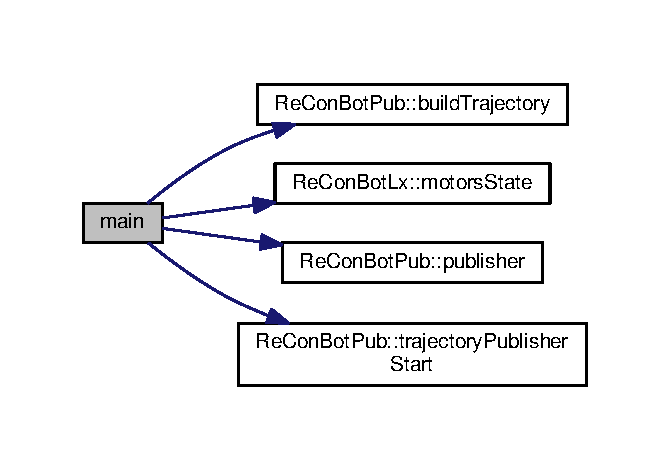
\includegraphics[width=322pt]{d5/d54/r__arm__trajectory__publisher_8cpp_a3c04138a5bfe5d72780bb7e82a18e627_cgraph}
\end{center}
\end{figure}

\hypertarget{_re_con_bot_8h}{}\section{Re\+Con\+Bot.\+h File Reference}
\label{_re_con_bot_8h}\index{Re\+Con\+Bot.\+h@{Re\+Con\+Bot.\+h}}
{\ttfamily \#include $<$pwd.\+h$>$}\newline
{\ttfamily \#include $<$sstream$>$}\newline
Include dependency graph for Re\+Con\+Bot.\+h\+:\nopagebreak
\begin{figure}[H]
\begin{center}
\leavevmode
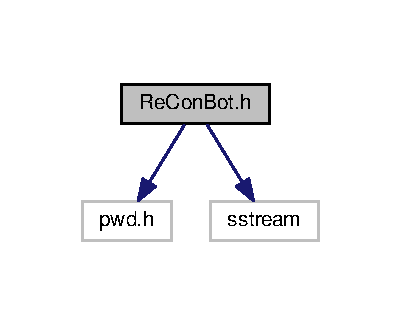
\includegraphics[width=193pt]{d7/d94/_re_con_bot_8h__incl}
\end{center}
\end{figure}
This graph shows which files directly or indirectly include this file\+:\nopagebreak
\begin{figure}[H]
\begin{center}
\leavevmode
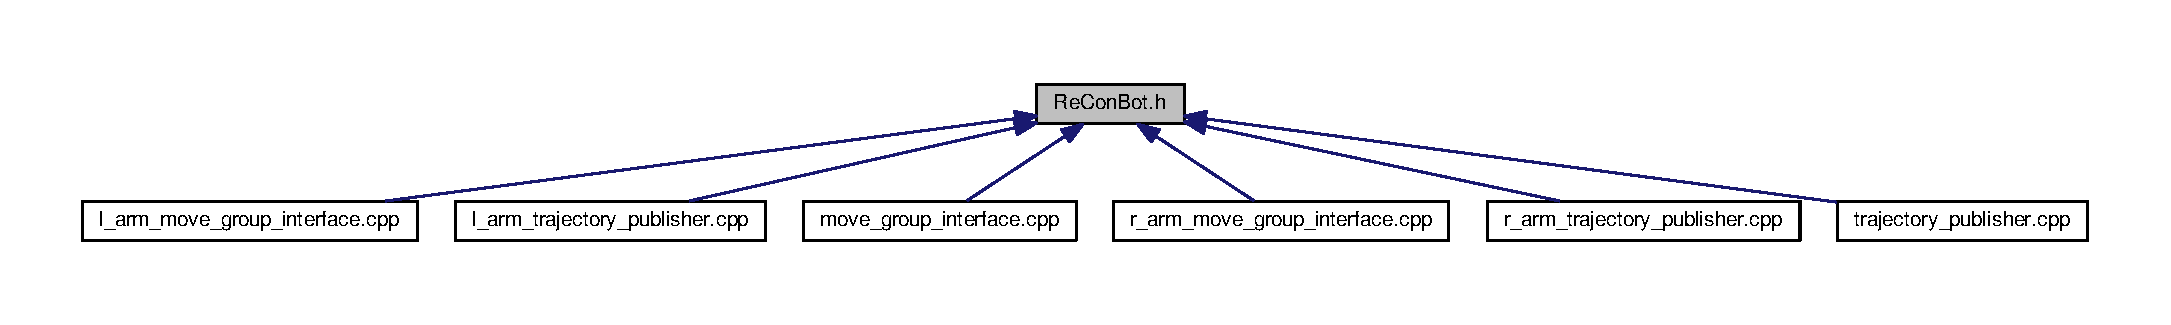
\includegraphics[width=350pt]{d0/d19/_re_con_bot_8h__dep__incl}
\end{center}
\end{figure}
\subsection*{Classes}
\begin{DoxyCompactItemize}
\item 
class \hyperlink{class_re_con_bot}{Re\+Con\+Bot}
\begin{DoxyCompactList}\small\item\em Class implemented for driving the \hyperlink{class_re_con_bot}{Re\+Con\+Bot} planning group. \end{DoxyCompactList}\item 
class \hyperlink{class_re_con_bot_lx}{Re\+Con\+Bot\+Lx}
\item 
class \hyperlink{class_re_con_bot_pub}{Re\+Con\+Bot\+Pub}
\end{DoxyCompactItemize}
\subsection*{Typedefs}
\begin{DoxyCompactItemize}
\item 
typedef actionlib\+::\+Simple\+Action\+Client$<$ control\+\_\+msgs\+::\+Follow\+Joint\+Trajectory\+Action $>$ \hyperlink{_re_con_bot_8h_a6fb8875093261cdc69e54d3ac7d5c301}{Traj\+Client}
\end{DoxyCompactItemize}
\subsection*{Variables}
\begin{DoxyCompactItemize}
\item 
static int \hyperlink{_re_con_bot_8h_af9fc8046227b67fb8c85827f5ebc4838}{n\+Motors}
\item 
static int $\ast$ \hyperlink{_re_con_bot_8h_a754c7486afa85fff30b8e7c0ce40c264}{motors\+Active}
\end{DoxyCompactItemize}


\subsection{Typedef Documentation}
\mbox{\Hypertarget{_re_con_bot_8h_a6fb8875093261cdc69e54d3ac7d5c301}\label{_re_con_bot_8h_a6fb8875093261cdc69e54d3ac7d5c301}} 
\index{Re\+Con\+Bot.\+h@{Re\+Con\+Bot.\+h}!Traj\+Client@{Traj\+Client}}
\index{Traj\+Client@{Traj\+Client}!Re\+Con\+Bot.\+h@{Re\+Con\+Bot.\+h}}
\subsubsection{\texorpdfstring{Traj\+Client}{TrajClient}}
{\footnotesize\ttfamily typedef actionlib\+::\+Simple\+Action\+Client$<$control\+\_\+msgs\+::\+Follow\+Joint\+Trajectory\+Action$>$ \hyperlink{basic__arm_8cpp_a6fb8875093261cdc69e54d3ac7d5c301}{Traj\+Client}}



Definition at line 53 of file Re\+Con\+Bot.\+h.



\subsection{Variable Documentation}
\mbox{\Hypertarget{_re_con_bot_8h_a754c7486afa85fff30b8e7c0ce40c264}\label{_re_con_bot_8h_a754c7486afa85fff30b8e7c0ce40c264}} 
\index{Re\+Con\+Bot.\+h@{Re\+Con\+Bot.\+h}!motors\+Active@{motors\+Active}}
\index{motors\+Active@{motors\+Active}!Re\+Con\+Bot.\+h@{Re\+Con\+Bot.\+h}}
\subsubsection{\texorpdfstring{motors\+Active}{motorsActive}}
{\footnotesize\ttfamily int$\ast$ motors\+Active\hspace{0.3cm}{\ttfamily [static]}}



Definition at line 55 of file Re\+Con\+Bot.\+h.



Referenced by Re\+Con\+Bot\+Pub\+::build\+Trajectory(), and Re\+Con\+Bot\+Lx\+::motors\+State().

\mbox{\Hypertarget{_re_con_bot_8h_af9fc8046227b67fb8c85827f5ebc4838}\label{_re_con_bot_8h_af9fc8046227b67fb8c85827f5ebc4838}} 
\index{Re\+Con\+Bot.\+h@{Re\+Con\+Bot.\+h}!n\+Motors@{n\+Motors}}
\index{n\+Motors@{n\+Motors}!Re\+Con\+Bot.\+h@{Re\+Con\+Bot.\+h}}
\subsubsection{\texorpdfstring{n\+Motors}{nMotors}}
{\footnotesize\ttfamily int n\+Motors\hspace{0.3cm}{\ttfamily [static]}}



Definition at line 54 of file Re\+Con\+Bot.\+h.



Referenced by Re\+Con\+Bot\+Pub\+::build\+Trajectory(), and Re\+Con\+Bot\+Lx\+::motors\+State().


\hypertarget{setup_8py}{}\section{setup.\+py File Reference}
\label{setup_8py}\index{setup.\+py@{setup.\+py}}
\subsection*{Namespaces}
\begin{DoxyCompactItemize}
\item 
 \hyperlink{namespacesetup}{setup}
\end{DoxyCompactItemize}
\subsection*{Variables}
\begin{DoxyCompactItemize}
\item 
\hyperlink{namespacesetup_aa2586b6c4dd84a0aaaf49cb1565cee6e}{setup.\+d}
\end{DoxyCompactItemize}

\hypertarget{trajectory__client_8py}{}\section{trajectory\+\_\+client.\+py File Reference}
\label{trajectory__client_8py}\index{trajectory\+\_\+client.\+py@{trajectory\+\_\+client.\+py}}
\subsection*{Classes}
\begin{DoxyCompactItemize}
\item 
class \hyperlink{classtrajectory__client_1_1_joint}{trajectory\+\_\+client.\+Joint}
\end{DoxyCompactItemize}
\subsection*{Namespaces}
\begin{DoxyCompactItemize}
\item 
 \hyperlink{namespacetrajectory__client}{trajectory\+\_\+client}
\end{DoxyCompactItemize}
\subsection*{Functions}
\begin{DoxyCompactItemize}
\item 
def \hyperlink{namespacetrajectory__client_a02f1f1cd99c608b8ea5167cb3c52a485}{trajectory\+\_\+client.\+main} ()
\end{DoxyCompactItemize}

\hypertarget{trajectory__publisher_8cpp}{}\section{trajectory\+\_\+publisher.\+cpp File Reference}
\label{trajectory__publisher_8cpp}\index{trajectory\+\_\+publisher.\+cpp@{trajectory\+\_\+publisher.\+cpp}}
{\ttfamily \#include $<$ros/ros.\+h$>$}\newline
{\ttfamily \#include $<$control\+\_\+msgs/\+Follow\+Joint\+Trajectory\+Action.\+h$>$}\newline
{\ttfamily \#include $<$actionlib/client/simple\+\_\+action\+\_\+client.\+h$>$}\newline
{\ttfamily \#include $<$iostream$>$}\newline
{\ttfamily \#include $<$fstream$>$}\newline
{\ttfamily \#include \char`\"{}Re\+Con\+Bot.\+h\char`\"{}}\newline
{\ttfamily \#include $<$string$>$}\newline
{\ttfamily \#include $<$vector$>$}\newline
{\ttfamily \#include $<$cstdlib$>$}\newline
{\ttfamily \#include $<$map$>$}\newline
{\ttfamily \#include $<$pwd.\+h$>$}\newline
Include dependency graph for trajectory\+\_\+publisher.\+cpp\+:\nopagebreak
\begin{figure}[H]
\begin{center}
\leavevmode
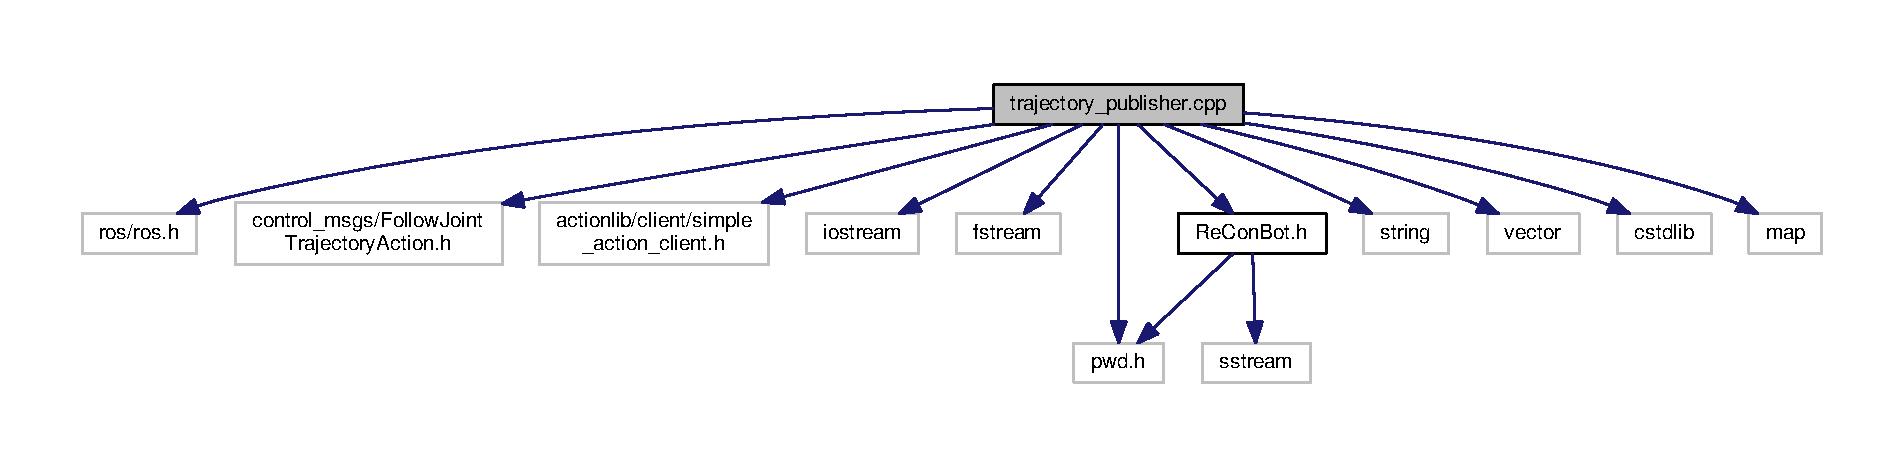
\includegraphics[width=350pt]{df/dd7/trajectory__publisher_8cpp__incl}
\end{center}
\end{figure}
\subsection*{Functions}
\begin{DoxyCompactItemize}
\item 
int \hyperlink{trajectory__publisher_8cpp_a3c04138a5bfe5d72780bb7e82a18e627}{main} (int argc, char $\ast$$\ast$argv)
\end{DoxyCompactItemize}


\subsection{Function Documentation}
\mbox{\Hypertarget{trajectory__publisher_8cpp_a3c04138a5bfe5d72780bb7e82a18e627}\label{trajectory__publisher_8cpp_a3c04138a5bfe5d72780bb7e82a18e627}} 
\index{trajectory\+\_\+publisher.\+cpp@{trajectory\+\_\+publisher.\+cpp}!main@{main}}
\index{main@{main}!trajectory\+\_\+publisher.\+cpp@{trajectory\+\_\+publisher.\+cpp}}
\subsubsection{\texorpdfstring{main()}{main()}}
{\footnotesize\ttfamily int main (\begin{DoxyParamCaption}\item[{int}]{argc,  }\item[{char $\ast$$\ast$}]{argv }\end{DoxyParamCaption})}



Definition at line 63 of file trajectory\+\_\+publisher.\+cpp.



References Re\+Con\+Bot\+Pub\+::build\+Trajectory(), Re\+Con\+Bot\+Lx\+::motors\+State(), Re\+Con\+Bot\+::name\+Space, Re\+Con\+Bot\+Pub\+::publisher(), Re\+Con\+Bot\+::source\+File, Re\+Con\+Bot\+::topic\+Name, and Re\+Con\+Bot\+Pub\+::trajectory\+Publisher\+Start().


\begin{DoxyCode}
63                               \{
64   ros::init(argc, argv, \textcolor{stringliteral}{"Trajectory\_Publisher"});
65   ros::NodeHandle nh;
66   control\_msgs::FollowJointTrajectoryGoal goal;
67   \textcolor{comment}{//ros::Rate loop\_rate(5);}
68   \textcolor{comment}{//ros::AsyncSpinner spinner(1);/**<Two spinner are instantiated for managing 2 threats*/}
69   \textcolor{comment}{//spinner.start();}
70   \hyperlink{class_re_con_bot_pub}{ReConBotPub} Publisher;
71   Publisher.\hyperlink{class_re_con_bot_a1d91d2ea8c0f16340440357906fb9ebf}{topicName} = \textcolor{stringliteral}{"/reconbot\_trajectory"};
72   \textcolor{keywordtype}{int} arg[] = \{1,2,3,4,5,6\};
73 
74   passwd* pw = getpwuid(getuid());
75   std::string path(pw->pw\_dir);
76 
77   Publisher.\hyperlink{class_re_con_bot_lx_a0e25f573057755c6729ea572362652e6}{motorsState}(arg,6);
78   Publisher.\hyperlink{class_re_con_bot_pub_a2019b0d8d30f2419026c90dd30de500f}{trajectoryPublisherStart}(nh, 1000);
79   Publisher.\hyperlink{class_re_con_bot_a40ca07cd606988b78664c4a52fd8dc59}{nameSpace} = \textcolor{stringliteral}{"reconbot\_controller"};
80   Publisher.\hyperlink{class_re_con_bot_a65cf4bed9bbabd92e1265d05507e0945}{sourceFile} = path += \textcolor{stringliteral}{"/catkin\_ws/src/reconbot/trajectory/trajectory.txt"};
81   goal = Publisher.\hyperlink{class_re_con_bot_pub_af99f5189cd8e834d7b59f1b106b99345}{buildTrajectory}();
82   Publisher.\hyperlink{class_re_con_bot_pub_ac763949cb5256de695e02c5f81084ead}{publisher}(goal);
83 
84   sleep(3);
85 
86   ROS\_INFO(\textcolor{stringliteral}{"Good bye!"});
87   \textcolor{comment}{//spinner.stop();}
88   \textcolor{comment}{//loop\_rate.sleep();}
89 
90   \textcolor{comment}{//sleep(2);}
91   \textcolor{keywordflow}{return} 0;
92 \}
\end{DoxyCode}
Here is the call graph for this function\+:\nopagebreak
\begin{figure}[H]
\begin{center}
\leavevmode
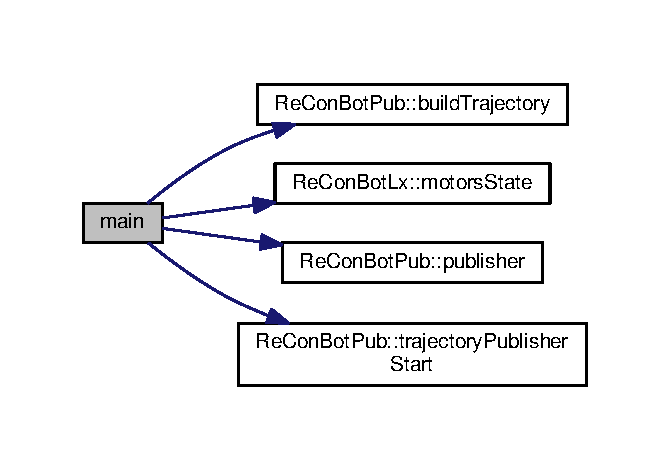
\includegraphics[width=322pt]{d7/d25/trajectory__publisher_8cpp_a3c04138a5bfe5d72780bb7e82a18e627_cgraph}
\end{center}
\end{figure}

%--- End generated contents ---

% Index
\backmatter
\newpage
\phantomsection
\clearemptydoublepage
\addcontentsline{toc}{chapter}{Index}
\printindex

\end{document}
